\documentclass[acmsmall,screen,review,anonymous,nonacm]{acmart}

\usepackage{amsthm}
\usepackage{enumitem}
\usepackage{listings}
\usepackage{xspace}
\usepackage{array}
\usepackage{mathtools}
\usepackage[export]{adjustbox}
\usepackage{flafter}
\usepackage{placeins}
\usepackage{needspace}

\ifdefined\directlua
  \setmainfont{Libertinus Serif}
  \setsansfont{Libertinus Sans}
  \setmathfont{Libertinus Math}[Scale=MatchUppercase]
  \setmonofont
{JetBrainsMono-Regular.ttf}[Path=fonts/,Scale=0.95,
RawFeature={-liga,-calt,-clig,-dlig}]
  \setmathrm{Libertinus Serif}
  \setmathsf{Libertinus Sans}
  \setmathtt
{JetBrainsMono-Regular.ttf}[Path=fonts/,Scale=0.95,
RawFeature={-liga,-calt,-clig,-dlig}]
  \renewcommand{\qedsymbol}{\ensuremath{\mdlgwhtsquare}}
\fi
\raggedbottom
\setlength{\parskip}{0pt}
\setlength{\textfloatsep}{10pt plus 2pt minus 2pt}
\setlength{\intextsep}{10pt plus 2pt minus 2pt}
\setlength{\floatsep}{8pt plus 2pt minus 2pt}
\renewcommand{\topfraction}{.9}
\renewcommand{\bottomfraction}{.8}
\renewcommand{\textfraction}{.1}
\renewcommand{\floatpagefraction}{.75}
\usepackage{tikz}
\usepackage{pgfplots}\pgfplotsset{compat=1.18}
\usetikzlibrary
{positioning,calc,arrows.meta,fit,backgrounds,
decorations.pathreplacing}
\usepackage{mathpartir}
\usepackage{cleveref}

\graphicspath{{./}}

\setlist{nosep, leftmargin=1.4em}

\newcommand{\pass}{X}
\newcommand{\back}{Y}
\newcommand{\body}{U}
\newcommand{\C}{\mathbb C}
\newcommand{\N}{\mathbb N}
\newcommand{\R}{\mathbb R}
\ifdefined\directlua
  \newfontface\storyinlineface
{JetBrainsMono-Regular.ttf}[Path=fonts/,Scale=MatchLowercase,
RawFeature={-liga,-calt,-clig,-dlig}]
  \IfFontExistsTF{fonts/JetBrainsMono-SemiBold.ttf}
    {\newfontface\storykwface
{JetBrainsMono-SemiBold.ttf}[Path=fonts/,Scale=0.95,
RawFeature={-liga,-calt,-clig,-dlig}]
     \newfontface\storyinlinekwface
{JetBrainsMono-SemiBold.ttf}[Path=fonts/,Scale=MatchLowercase,
RawFeature={-liga,-calt,-clig,-dlig}]}
    {\newcommand{\storykwface}{\ttfamily\bfseries}
     \newcommand{\storyinlinekwface}{\storyinlineface\bfseries}}
\else
  \newcommand{\storykwface}{\ttfamily\bfseries}
  \newcommand{\storyinlineface}{\small\ttfamily}
  \newcommand{\storyinlinekwface}{\small\ttfamily\bfseries}
\fi
\newcommand{\kw}[1]{\textnormal{\storyinlinekwface #1}}
\newcommand{\code}[1]{\textnormal{\storyinlineface #1}}
\newcommand{\loopc}{\kw{loop}\xspace}
\newcommand{\countc}{\kw{count}\xspace}
\newcommand{\whilec}{\kw{while}\xspace}
\newcommand{\tr}{\operatorname{tr}}
\DeclareMathOperator{\Tr}{Tr}
\DeclareMathOperator{\rank}{rank}
\newcommand{\Loop}{\Tr}
\newcommand{\exitmap}[1]{x_{#1}}
\newcommand{\seq}{\mathbin{;}}
\providecommand{\llbracket}{[\![}
\providecommand{\rrbracket}{]\!]}
\newcommand{\sem}[1]{\llbracket #1 \rrbracket}
\newcommand{\ket}[1]{\lvert #1\rangle}
\newcommand{\bra}[1]{\langle #1\rvert}
\newcommand{\inner}[2]{\langle #1, #2 \rangle}

\definecolor{flipout}{HTML}{007A59}
\definecolor{flipback}{HTML}{7A3E65}
\definecolor{equalcount}{HTML}{006A91}
\definecolor{othercount}{HTML}{777777}
\definecolor{ink}{HTML}{1F2328}
\definecolor{quiet}{gray}{0.45}
\definecolor{muted}{HTML}{5B6470}
\definecolor{accent}{HTML}{006A91}
\definecolor{accentsoft}{HTML}{E8EEF4}
\definecolor{accentwarm}{HTML}{9A5B00}
\definecolor{accentplum}{HTML}{70355C}
\definecolor{hairline}{HTML}{C9CFD6}
\definecolor{judgerule}{HTML}{231F20}
\definecolor{boxfill}{HTML}{FFFEF8}
\definecolor{hlblue}{HTML}{DAF3FD}

\tikzset{
house/.style={>={Stealth[length=2.1mm, width=1.6mm]}, line
width=0.5pt, node distance=9mm and 15mm, every
node/.style={font=\small}}, box/.style={draw=ink, line width=0.5pt,
rounded corners=1.5pt, inner xsep=6pt, inner ysep=4pt, align=center},
boxhi/.style={box, draw=accent, fill=accentsoft, text=ink},
boxdim/.style={box, draw=hairline, text=muted}, flow/.style={->,
draw=ink}, lbl/.style={font=\footnotesize\itshape, text=accent, inner
sep=2pt}, lbldim/.style={font=\footnotesize, text=muted, inner
sep=2pt}, group/.style={draw=hairline, dashed, rounded corners=2pt,
inner sep=7pt}, hid/.style={draw=muted, dashed, dash pattern=on 1.6pt
off 1.3pt, line width=0.5pt}, void/.style={circle, draw=muted,
fill=white, line width=0.5pt, inner sep=1.1pt}, med/.style={box,
inner xsep=3pt, inner ysep=2pt, draw=accent, text=accent},
wire/.style={draw=ink, line width=0.6pt}, cwire/.style={double,
draw=ink, line width=0.4pt}, dot/.style={circle, fill=ink, inner
sep=0pt, minimum size=1.5mm}, dothi/.style={circle, fill=accent,
inner sep=0pt, minimum size=1.7mm}, wlab/.style={font=\footnotesize,
text=ink, inner sep=1.5pt}, hlab/.style={font=\footnotesize,
text=muted, inner sep=1.5pt},
}


\tikzset{
kme circuit/.style={x=1cm,y=1cm,every node/.style={font=\small,inner
sep=2pt}}, kme wire/.style={draw=ink,line width=.65pt}, kme
gate/.style={draw=ink,fill=white,minimum width=7mm,minimum
height=5.5mm,inner sep=2pt}, kme dot/.style={circle,fill=ink,minimum
size=4pt,inner sep=0pt}, kme
open/.style={circle,draw=ink,fill=white,minimum size=5pt,inner
sep=0pt}
}
\definecolor{svpass}{HTML}{007A59}
\definecolor{svpasssoft}{HTML}{DAF1E9}
\definecolor{svback}{HTML}{7A3E65}
\definecolor{svbacksoft}{HTML}{F1E1EB}
\definecolor{svkeep}{HTML}{006A91}
\definecolor{svkeepsoft}{HTML}{DCE9F5}
\definecolor{svmeas}{HTML}{9A5B00}
\definecolor{svmeassoft}{HTML}{FBEFD5}
\tikzset{
sv/base/.style={>={Stealth[length=1.25mm,width=.85mm]},line
width=.55pt,every node/.style={font=\small,inner sep=2pt}},
sv/state/.style={draw=ink,rounded
corners=2pt,fill=white,align=center,inner xsep=4pt,inner ysep=3pt},
sv/pass/.style={sv/state,draw=svpass,shade,left color=white,right
color=svpasssoft}, sv/back/.style={sv/state,draw=svback,shade,left
color=white,right color=svbacksoft},
sv/keep/.style={sv/state,draw=svkeep,shade,left color=white,right
color=svkeepsoft}, sv/meas/.style={sv/state,draw=svmeas,shade,left
color=white,right color=svmeassoft}, sv/flow/.style={->,draw=ink},
sv/return/.style={->,draw=svback},
sv/note/.style={font=\footnotesize,text=muted,align=center},
sv/head/.style={font=\footnotesize\sffamily,text=muted,anchor=west},
sv/gate/.style={sv/state,minimum size=6mm,inner sep=2pt}
}
\newlength{\storyrowwidth}
\newcommand{\storysourceview}[3][.51]{\par\smallskip\noindent
\begingroup
 \setlength{\storyrowwidth}{\linewidth}\begin
{minipage}[c]{#1\storyrowwidth}
 \lstset
{xleftmargin=0pt,breaklines=true,breakatwhitespace=true,
breakindent=1em}#2
 \end{minipage}\hfill
 \begin{minipage}[c]{\dimexpr\storyrowwidth-#1\storyrowwidth
-.03\storyrowwidth\relax}
 \centering #3
 \end{minipage}\endgroup\par\smallskip}

\newcommand{\storyIntroFlipView}{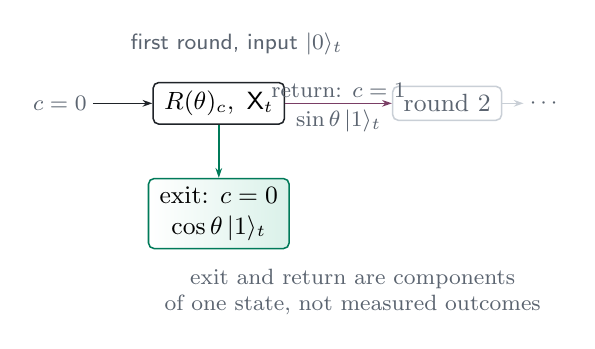
\begin{tikzpicture}[sv/base]
 \node[sv/head] at (-1.2,1.6) {first round, input $\ket0_t$};
 \node[sv/state] (t1) at (0,.85) {$R(\theta)_c,\ \mathsf X_t$};
 \node[sv/state,draw=hairline,text=muted] (t2) at (2.9,.85) {round
 2};
 \node[sv/note] (t3) at (4.15,.85) {$\cdots$};
 \draw[sv/flow] (-1.6,.85) node[left,sv/note] {$c=0$} -- (t1.west);
 \draw[sv/return] (t1.east) -- node[above,sv/note] {return: $c=1$}
 node[below,sv/note] {$\sin\theta\,\ket1_t$} (t2.west);
 \draw[sv/flow,draw=hairline] (t2.east) -- (t3.west);
 \node[sv/pass] (x0) at (0,-.55) {exit:
 $c=0$\\$\cos\theta\,\ket1_t$};
 \draw[sv/flow,svpass] (t1.south) -- (x0.north);
 \node[sv/note] at (1.7,-1.55) {exit and return are components\\of
 one state, not measured outcomes};
\end{tikzpicture}}

\newcommand{\storyFlipEraseView}{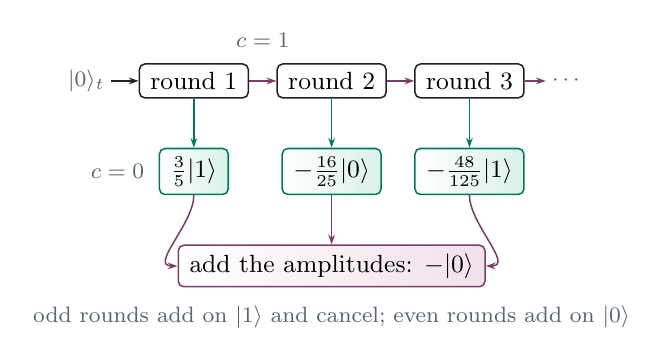
\begin{tikzpicture}[sv/base]
 \node[sv/state] (t1) at (0,.85) {round 1};
 \node[sv/state] (t2) at (1.75,.85) {round 2};
 \node[sv/state] (t3) at (3.5,.85) {round 3};
 \node[sv/note] (t4) at (4.75,.85) {$\cdots$};
 \draw[sv/flow] (-1.05,.85) node[left,sv/note] {$\ket0_t$} --
 (t1.west);
 \draw[sv/return] (t1.east) -- (t2.west);
 \node[sv/note,anchor=south] at ($(t1.north east)!.5!(t2.north
 west)+(0,.12)$) {$c=1$};
 \draw[sv/return] (t2.east) -- (t3.west);
 \draw[sv/return] (t3.east) -- (t4.west);
 \node[sv/pass] (x0) at (0,-.3) {$\tfrac35\ket1$};
 \node[sv/note,anchor=east] at ([xshift=-3pt]x0.west) {$c=0$};
 \node[sv/pass] (x1) at (1.75,-.3) {$-\tfrac{16}{25}\ket0$};
 \node[sv/pass] (x2) at (3.5,-.3) {$-\tfrac{48}{125}\ket1$};
 \draw[sv/flow,svpass] (t1.south) -- (x0.north);
 \draw[sv/flow,svpass] (t2.south) -- (x1.north);
 \draw[sv/flow,svpass] (t3.south) -- (x2.north);
 \node[sv/back] (sum) at (1.75,-1.5) {add the amplitudes: $-\ket0$};
 \draw[sv/flow,svback] (x0.south) to[out=-90,in=180] (sum.west);
 \draw[sv/flow,svback] (x1.south) -- (sum.north);
 \draw[sv/flow,svback] (x2.south) to[out=-90,in=0] (sum.east);
 \node[sv/note] at (1.75,-2.15) {odd rounds add on $\ket1$ and
 cancel; even rounds add on $\ket0$};
\end{tikzpicture}}

\newcommand{\storyFlipWhileView}{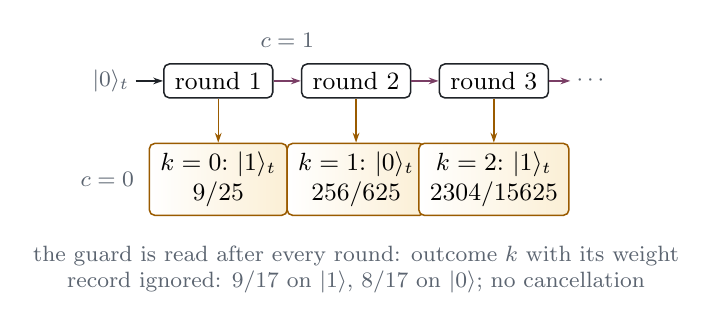
\begin{tikzpicture}[sv/base]
 \node[sv/state] (t1) at (0,.85) {round 1};
 \node[sv/state] (t2) at (1.75,.85) {round 2};
 \node[sv/state] (t3) at (3.5,.85) {round 3};
 \node[sv/note] (t4) at (4.75,.85) {$\cdots$};
 \draw[sv/flow] (-1.05,.85) node[left,sv/note] {$\ket0_t$} --
 (t1.west);
 \draw[sv/return] (t1.east) -- (t2.west);
 \node[sv/note,anchor=south] at ($(t1.north east)!.5!(t2.north
 west)+(0,.12)$) {$c=1$};
 \draw[sv/return] (t2.east) -- (t3.west);
 \draw[sv/return] (t3.east) -- (t4.west);
 \node[sv/meas] (x0) at (0,-.4) {$k=0$:\ $\ket1_t$\\$9/25$};
 \node[sv/note,anchor=east] at ([xshift=-3pt]x0.west) {$c=0$};
 \node[sv/meas] (x1) at (1.75,-.4) {$k=1$:\ $\ket0_t$\\$256/625$};
 \node[sv/meas] (x2) at (3.5,-.4) {$k=2$:\ $\ket1_t$\\$2304/15625$};
 \draw[sv/flow,svmeas] (t1.south) -- (x0.north);
 \draw[sv/flow,svmeas] (t2.south) -- (x1.north);
 \draw[sv/flow,svmeas] (t3.south) -- (x2.north);
 \node[sv/note] at (1.75,-1.55) {the guard is read after every round:
 outcome $k$ with its weight\\record ignored: $9/17$ on $\ket1$,
 $8/17$ on $\ket0$; no cancellation};
\end{tikzpicture}}

\newcommand{\storyFlipCountView}{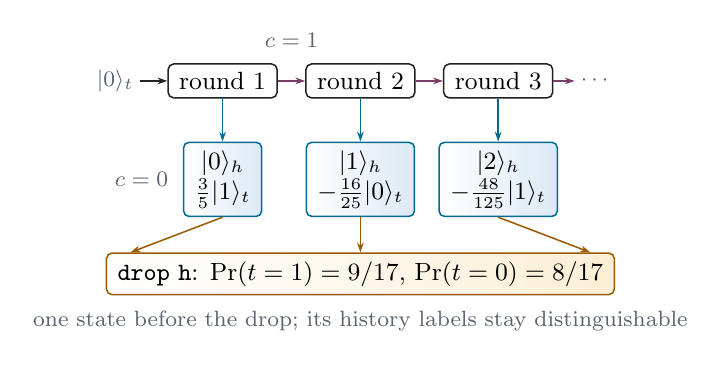
\begin{tikzpicture}[sv/base]
 \node[sv/state] (t1) at (0,.85) {round 1};
 \node[sv/state] (t2) at (1.75,.85) {round 2};
 \node[sv/state] (t3) at (3.5,.85) {round 3};
 \node[sv/note] (t4) at (4.75,.85) {$\cdots$};
 \draw[sv/flow] (-1.05,.85) node[left,sv/note] {$\ket0_t$} --
 (t1.west);
 \draw[sv/return] (t1.east) -- (t2.west);
 \node[sv/note,anchor=south] at ($(t1.north east)!.5!(t2.north
 west)+(0,.12)$) {$c=1$};
 \draw[sv/return] (t2.east) -- (t3.west);
 \draw[sv/return] (t3.east) -- (t4.west);
 \node[sv/keep] (x0) at (0,-.4) {$\ket0_h$\\$\tfrac35\ket1_t$};
 \node[sv/note,anchor=east] at ([xshift=-3pt]x0.west) {$c=0$};
 \node[sv/keep] (x1) at (1.75,-.4)
 {$\ket1_h$\\$-\tfrac{16}{25}\ket0_t$};
 \node[sv/keep] (x2) at (3.5,-.4)
 {$\ket2_h$\\$-\tfrac{48}{125}\ket1_t$};
 \draw[sv/flow,svkeep] (t1.south) -- (x0.north);
 \draw[sv/flow,svkeep] (t2.south) -- (x1.north);
 \draw[sv/flow,svkeep] (t3.south) -- (x2.north);
 \node[sv/meas] (out) at (1.75,-1.6) {\kw{drop} \code{h}:
 $\Pr(t=1)=9/17$, $\Pr(t=0)=8/17$};
 \draw[sv/flow,svmeas] (x0.south) -- ([xshift=9pt]out.north west);
 \draw[sv/flow,svmeas] (x1.south) -- (out.north);
 \draw[sv/flow,svmeas] (x2.south) -- ([xshift=-9pt]out.north east);
 \node[sv/note] at (1.75,-2.2) {one state before the drop; its
 history labels stay distinguishable};
\end{tikzpicture}}

\newcommand{\storyCycleView}{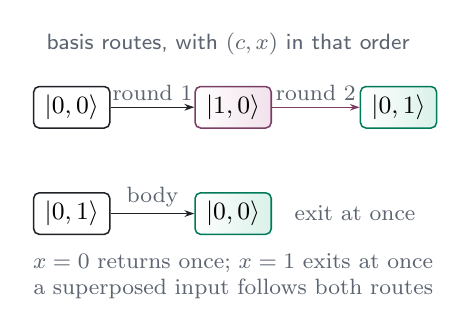
\begin{tikzpicture}[sv/base]
 \node[sv/head] at (-.1,1.6) {basis routes, with $(c,x)$ in that
 order};
 \node[sv/state] (i0) at (.3,.8) {$\ket{0,0}$};
 \node[sv/back] (r) at (2.35,.8) {$\ket{1,0}$};
 \node[sv/pass] (o1) at (4.45,.8) {$\ket{0,1}$};
 \draw[sv/flow] (i0.east) -- node[above,sv/note] {round 1} (r.west);
 \draw[sv/return] (r.east) -- node[above,sv/note] {round 2}
 (o1.west);
 \node[sv/state] (i1) at (.3,-.55) {$\ket{0,1}$};
 \node[sv/pass] (o0) at (2.35,-.55) {$\ket{0,0}$};
 \draw[sv/flow] (i1.east) -- node[above,sv/note] {body} (o0.west);
 \node[sv/note,anchor=west] at (3.05,-.55) {exit at once};
 \node[sv/note] at (2.35,-1.35) {$x=0$ returns once; $x=1$ exits at
 once\\a superposed input follows both routes};
\end{tikzpicture}}

\newcommand{\storyReflectionView}{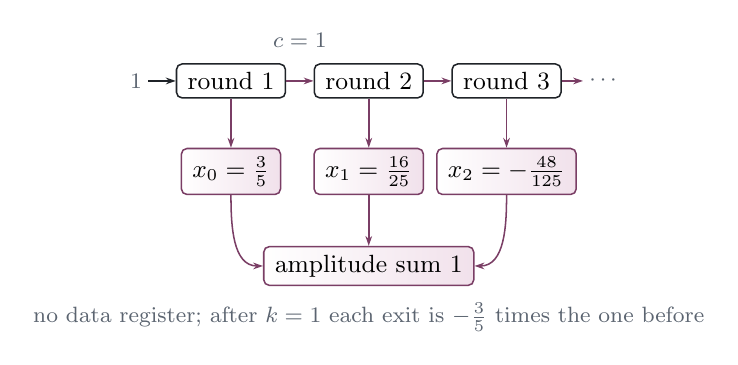
\begin{tikzpicture}[sv/base]
 \node[sv/state] (t1) at (0,.85) {round 1};
 \node[sv/state] (t2) at (1.75,.85) {round 2};
 \node[sv/state] (t3) at (3.5,.85) {round 3};
 \node[sv/note] (t4) at (4.75,.85) {$\cdots$};
 \draw[sv/flow] (-1.05,.85) node[left,sv/note] {$1$} -- (t1.west);
 \draw[sv/return] (t1.east) -- (t2.west);
 \node[sv/note,anchor=south] at ($(t1.north east)!.5!(t2.north
 west)+(0,.12)$) {$c=1$};
 \draw[sv/return] (t2.east) -- (t3.west);
 \draw[sv/return] (t3.east) -- (t4.west);
 \node[sv/back] (x0) at (0,-.3) {$x_0=\tfrac35$};
 \node[sv/back] (x1) at (1.75,-.3) {$x_1=\tfrac{16}{25}$};
 \node[sv/back] (x2) at (3.5,-.3) {$x_2=-\tfrac{48}{125}$};
 \draw[sv/flow,svback] (t1.south) -- (x0.north);
 \draw[sv/flow,svback] (t2.south) -- (x1.north);
 \draw[sv/flow,svback] (t3.south) -- (x2.north);
 \node[sv/back] (sum) at (1.75,-1.5) {amplitude sum $1$};
 \draw[sv/flow,svback] (x0.south) to[out=-90,in=180] (sum.west);
 \draw[sv/flow,svback] (x1.south) -- (sum.north);
 \draw[sv/flow,svback] (x2.south) to[out=-90,in=0] (sum.east);
 \node[sv/note] at (1.75,-2.15) {no data register; after $k=1$ each
 exit is $-\tfrac35$ times the one before};
\end{tikzpicture}}

\newcommand{\storyApplyHView}{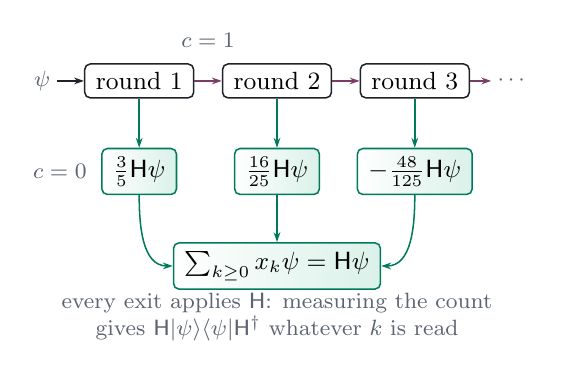
\begin{tikzpicture}[sv/base]
 \node[sv/state] (t1) at (0,.85) {round 1};
 \node[sv/state] (t2) at (1.75,.85) {round 2};
 \node[sv/state] (t3) at (3.5,.85) {round 3};
 \node[sv/note] (t4) at (4.75,.85) {$\cdots$};
 \draw[sv/flow] (-1.05,.85) node[left,sv/note] {$\psi$} -- (t1.west);
 \draw[sv/return] (t1.east) -- (t2.west);
 \node[sv/note,anchor=south] at ($(t1.north east)!.5!(t2.north
 west)+(0,.12)$) {$c=1$};
 \draw[sv/return] (t2.east) -- (t3.west);
 \draw[sv/return] (t3.east) -- (t4.west);
 \node[sv/pass] (x0) at (0,-.3) {$\tfrac35\mathsf H\psi$};
 \node[sv/note,anchor=east] at ([xshift=-3pt]x0.west) {$c=0$};
 \node[sv/pass] (x1) at (1.75,-.3) {$\tfrac{16}{25}\mathsf H\psi$};
 \node[sv/pass] (x2) at (3.5,-.3) {$-\tfrac{48}{125}\mathsf H\psi$};
 \draw[sv/flow,svpass] (t1.south) -- (x0.north);
 \draw[sv/flow,svpass] (t2.south) -- (x1.north);
 \draw[sv/flow,svpass] (t3.south) -- (x2.north);
 \node[sv/pass] (sum) at (1.75,-1.5) {$\sum_{k\geq0}x_k\psi=\mathsf
 H\psi$};
 \draw[sv/flow,svpass] (x0.south) to[out=-90,in=180] (sum.west);
 \draw[sv/flow,svpass] (x1.south) -- (sum.north);
 \draw[sv/flow,svpass] (x2.south) to[out=-90,in=0] (sum.east);
 \node[sv/note] at (1.75,-2.15) {every exit applies $\mathsf H$:
 measuring the count\\gives $\mathsf H\ket\psi\bra\psi\mathsf
 H^\dagger$ whatever $k$ is read};
\end{tikzpicture}}

\newcommand{\storyBodyPhaseView}{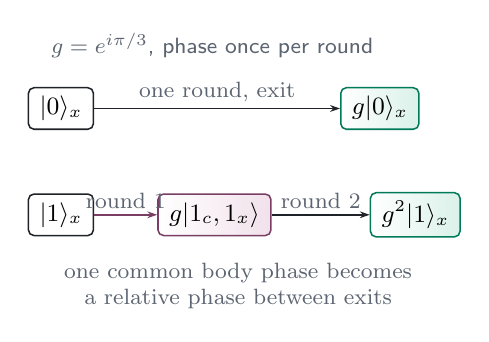
\begin{tikzpicture}[sv/base]
 \node[sv/head] at (-.1,1.6) {$g=e^{i\pi/3}$, phase once per round};
 \node[sv/state] (i0) at (.1,.8) {$\ket0_x$};
 \node[sv/pass] (o0) at (4.15,.8) {$g\ket0_x$};
 \draw[sv/flow] (i0.east) -- node[above,sv/note] {one round, exit}
 (o0.west);
 \node[sv/state] (i1) at (.1,-.55) {$\ket1_x$};
 \node[sv/back] (r) at (2.05,-.55) {$g\ket{1_c,1_x}$};
 \node[sv/pass] (o1) at (4.6,-.55) {$g^2\ket1_x$};
 \draw[sv/return] (i1.east) -- node[above,sv/note] {round 1}
 (r.west);
 \draw[sv/flow] (r.east) -- node[above,sv/note] {round 2} (o1.west);
 \node[sv/note] at (2.35,-1.45) {one common body phase becomes\\a
 relative phase between exits};
\end{tikzpicture}}

\newcommand{\storyKickbackView}{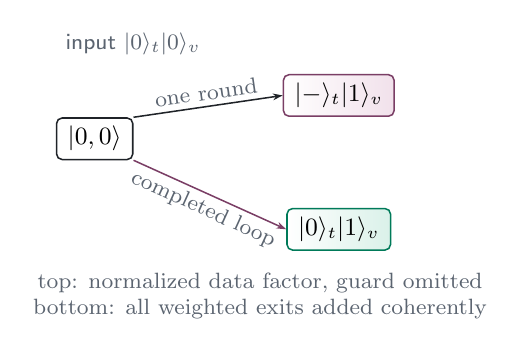
\begin{tikzpicture}[sv/base]
 \node[sv/head] at (-.1,1.65) {input $\ket0_t\ket0_v$};
 \node[sv/state] (in) at (.35,.45) {$\ket{0,0}$};
 \node[sv/back] (first) at (3.45,1.0) {$\ket-_t\ket1_v$};
 \node[sv/pass] (sum) at (3.45,-.7) {$\ket0_t\ket1_v$};
 \draw[sv/flow] (in.north east) -- node[above,sv/note,sloped] {one
 round} (first.west);
 \draw[sv/flow,svback] (in.south east) -- node[below,sv/note,sloped]
 {completed loop} (sum.west);
 \node[sv/note] at (2.45,-1.55) {top: normalized data factor, guard
 omitted\\bottom: all weighted exits added coherently};
\end{tikzpicture}}

\newcommand{\storyFringeView}{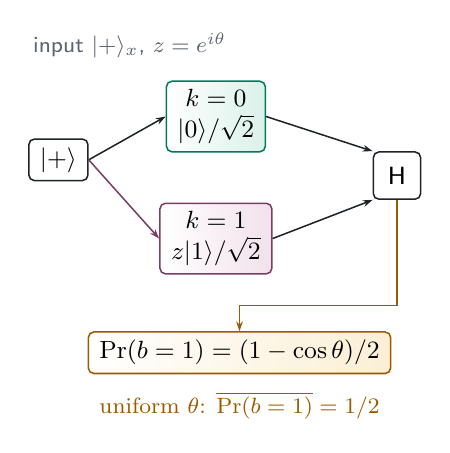
\begin{tikzpicture}[sv/base]
 \node[sv/head] at (-.1,2.05) {input $\ket+_x$, $z=e^{i\theta}$};
 \node[sv/state] (in) at (.3,.6) {$\ket+$};
 \node[sv/pass] (a) at (2.3,1.15) {$k=0$\\$\ket0/\sqrt2$};
 \node[sv/back] (b) at (2.3,-.4) {$k=1$\\$z\ket1/\sqrt2$};
 \node[sv/gate] (h) at (4.6,.4) {$\mathsf H$};
 \draw[sv/flow] (in.east) -- (a.west);
 \draw[sv/return] (in.east) -- (b.west);
 \draw[sv/flow] (a.east) -- (h.north west);
 \draw[sv/flow] (b.east) -- (h.south west);
 \node[sv/meas] (out) at (2.6,-1.85) {$\Pr(b=1)=(1-\cos\theta)/2$};
 \draw[sv/flow,svmeas] (h.south) -- (4.6,-1.25) -| (out.north);
 \node[sv/note,text=svmeas] at (2.6,-2.52)
  {uniform $\theta$: $\overline{\Pr(b=1)}=1/2$};
\end{tikzpicture}}

\newcommand{\storyWeightView}{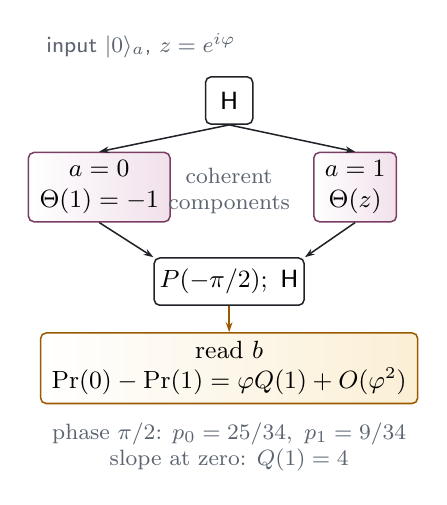
\begin{tikzpicture}[sv/base]
 \node[sv/head] at (-.1,2.1) {input $\ket0_a$, $z=e^{i\varphi}$};
 \node[sv/gate] (h) at (2.3,1.4) {$\mathsf H$};
 \node[sv/back] (a) at (.65,.3) {$a=0$\\$\Theta(1)=-1$};
 \node[sv/back] (b) at (3.9,.3) {$a=1$\\$\Theta(z)$};
 \draw[sv/flow] (h.south) -- (a.north);
 \draw[sv/flow] (h.south) -- (b.north);
 \node[sv/note] at (2.3,.25) {coherent\\components};
 \node[sv/gate] (read) at (2.3,-.9) {$P(-\pi/2);\ \mathsf H$};
 \draw[sv/flow] (a.south) -- (read.north west);
 \draw[sv/flow] (b.south) -- (read.north east);
 \node[sv/meas] (bit) at (2.3,-2.0) {read $b$\\$\Pr(0)-\Pr(1)=\varphi
 Q(1)+O(\varphi^2)$};
 \draw[sv/flow,svmeas] (read.south) -- (bit.north);
 \node[sv/note] at (2.3,-3.0) {phase $\pi/2$: $p_0=25/34,\
 p_1=9/34$\\slope at zero: $Q(1)=4$};
\end{tikzpicture}}

\newcommand{\storyRingReferenceView}{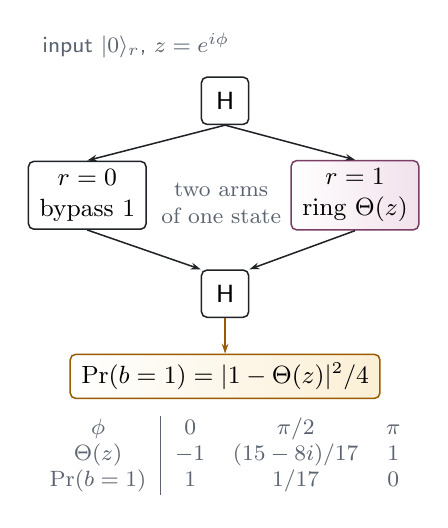
\begin{tikzpicture}[sv/base]
 \node[sv/head] at (-.1,2.2) {input $\ket0_r$, $z=e^{i\phi}$};
 \node[sv/gate] (h) at (2.3,1.5) {$\mathsf H$};
 \node[sv/state] (a) at (.55,.3) {$r=0$\\bypass $1$};
 \node[sv/back] (b) at (3.95,.3) {$r=1$\\ring $\Theta(z)$};
 \draw[sv/flow] (h.south) -- (a.north);
 \draw[sv/flow] (h.south) -- (b.north);
 \node[sv/note] at (2.25,.2) {two arms\\of one state};
 \node[sv/gate] (read) at (2.3,-.95) {$\mathsf H$};
 \draw[sv/flow] (a.south) -- (read.north west);
 \draw[sv/flow] (b.south) -- (read.north east);
 \node[sv/meas] (bit) at (2.3,-2.0) {$\Pr(b=1)=|1-\Theta(z)|^2/4$};
 \draw[sv/flow,svmeas] (read.south) -- (bit.north);
 \node[sv/note] at (2.3,-3.0) {$\begin{array}{c|ccc}
 \phi&0&\pi/2&\pi\\
 \Theta(z)&-1&(15-8i)/17&1\\
 \Pr(b=1)&1&1/17&0
 \end{array}$};
\end{tikzpicture}}
\newcommand{\storyUndoView}{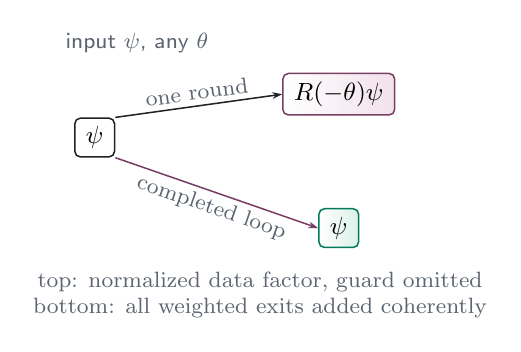
\begin{tikzpicture}[sv/base]
 \node[sv/head] at (-.1,1.65) {input $\psi$, any $\theta$};
 \node[sv/state] (in) at (.35,.45) {$\psi$};
 \node[sv/back] (first) at (3.45,1.0) {$R(-\theta)\psi$};
 \node[sv/pass] (sum) at (3.45,-.7) {$\psi$};
 \draw[sv/flow] (in.north east) -- node[above,sv/note,sloped] {one
 round} (first.west);
 \draw[sv/flow,svback] (in.south east) -- node[below,sv/note,sloped]
 {completed loop} (sum.west);
 \node[sv/note] at (2.45,-1.55) {top: normalized data factor, guard
 omitted\\bottom: all weighted exits added coherently};
\end{tikzpicture}}
\newcommand{\isorule}[2]{\inferrule{#1}{#2}}
\numberwithin{equation}{section}
\settopmatter{printacmref=false, printfolios=true}
\setcopyright{none}
\acmConference[PLDI]{ACM SIGPLAN Conference on Programming Language
Design and Implementation}{}{}
\acmYear{2027}


\newenvironment{programfigure}
 {\par\addvspace{\intextsep}\noindent\begin{minipage}{\linewidth
}\captionsetup{hypcap=false,type=figure}\centering}
 {\end{minipage}\par\addvspace{\intextsep}}
\newcommand{\picdir}{figures}
\newcommand{\pic}[3]{\par\begin{figure}[!htbp]\centering
  \includegraphics[max width=\linewidth]{\picdir/#1.pdf}
  \caption{#2}\label{fig:#1}\Description{#3}\end{figure}\par}
\newcommand{\sheetpic}[3]{{\renewcommand{\picdir}{figures}\pic
{#1}{#2}{#3}}}
\newcommand{\clocktype}{[K]}
\newcommand{\chan}[1]{\mathcal E_{#1}}
\newcommand{\Id}{\mathrm{id}}
\newcommand{\rec}{\mathcal R}
\newcommand{\meas}{\mathcal M}
\newcommand{\Int}{\mathrm{Int}}
\lstdefinelanguage
{iso}{morekeywords={let,in,round,exit,back,left,right,
unit,loop,trace,while,count,alloc,discard},sensitive=true}
\lstset{language=iso,basicstyle=\ttfamily\small
,keywordstyle=\storykwface,
columns=fullflexible,keepspaces=true,xleftmargin=1em,
showstringspaces=false,
aboveskip=.45\baselineskip,belowskip=.45\baselineskip}
\setcitestyle{numbers,sort&compress}
\lstset{literate={<}{{\ensuremath{\langle}}}1
                 {>}{{\ensuremath{\rangle}}}1
                 {<->}{{\ensuremath{\leftrightarrow}}}2}
\begin{document}
\title{Keep, Measure, Erase}
\subtitle{What a Quantum Loop Does with Its History}
\author{Anonymous Author(s)}
\affiliation{\institution{}\city{}\country{}}
\maketitle
\hypersetup{citecolor=ink,linkcolor=ink,urlcolor=muted}

\section{Introduction}
Suppose we want to know how many iterations a loop went through
before halting, and we want that number without changing its output
or what the loop actually did. In a classical program we can just
allocate and increment a private counter as the body goes through
each iteration and keep or ignore it when the loop finishes. This
remains a valid way to get the iteration count even if the body
tosses a coin to decide whether to continue. A terminating execution
still goes through the body a definite number of times, so recording
that number changes neither its returned value nor the probability of
obtaining that value.

For a quantum program, recording the number of iterations can change
the loop's output behaviour. A body operating on a quantum guard may
send amplitude both out of the loop and back for another call. If the
contributions leaving after different numbers of calls reach the same
output, their complex amplitudes add before a measurement assigns
concrete probabilities. A counter puts these contributions alongside
orthogonal labels, which distinguish them even if nobody reads the
counter. Ignoring it means observing only the returned data, whose
state is obtained by tracing out that register. This removes the
terms between different count labels. We ask when recording and
discarding the count preserves every observation on the returned
data: when does the loop with a record give the same data as coherent
feedback?

We start with a finite unitary body $U:X\oplus Y\to X'\oplus Y$,
connecting its output $Y$ to its input $Y$. The established
direct-sum trace adds what leaves after every possible number of
returns, as in reversible iteration and geometry of
interaction~\cite
{JamesSabry13Interpreters,AbramskyHaghverdiScott02GoI,JSV96}.
On finite unitary bodies it gives a unitary external map even when
infinitely many rounds
contribute~\cite
{Bartha14QuantumTuringAutomata,AndresMartinez22Thesis}.
We use this trace to interpret coherent feedback
(Section~\ref{sec:trace}).

We use symmetric pattern matching to write programs over the finite
sum and product types of $\Pi$ (Section~\ref{sec:iso}). Classical
$\Pi$ expresses finite bijections; its quantum extensions express
unitary gates, with approximate universality for $\mathrm
U\Pi$~\cite[\S\S~3.1--3.2]{HeunenKaarsgaard22Effects}. Our finite
clause presentation admits exact complex coefficients, and we add
$\mathsf{trace}$ for coherent feedback. Following \emph{Quantum
Information Effects}~\cite[\S\S~3--4]{HeunenKaarsgaard22Effects}, we
add allocation to supply a counter for the recording loop, and hiding
to discard outputs and derive the guard measurement used on each
turn~\cite[\S~3]{YingFeng10QuantumLoop} (Section~\ref{sec:effects}).
Allocation lets a program return a counter with its data as a
norm-preserving isometry. Hiding that register gives a channel on the
remaining data. A finite cyclic counter records the count modulo its
size, and an exact count is their countable semantic limit.
Discarding the exact record gives the channel of measuring the guard
on every call.

We write $L$ for the coherent loop and $x_k$ for the linear map that
takes an input $u$ to the amplitude contribution $x_ku$ leaving after
$k$ returns. In Section~\ref{sec:agreement} we give a finite test for
equality of the measured channel and $\rho\mapsto L\rho L^\dagger$,
permitting replacement in any channel context, including data
entangled with a reference the caller keeps. It passes exactly when
every exit is a scalar multiple of $L$, and checking the first $m+1$
exits suffices, with $m=\dim Y$. Then the record has a fixed state
independent of the data. Kraus proportionality for finite families is
known~\cite[Cor.~2.23]{Watrous18TQI}; our comparison connects it to
an exit sequence, a finite check and a typed replacement.

This leaves a second question: what can we learn about the rounds of
a loop that keeps no count (Section~\ref{sec:phase})? A phase on the
return wire marks each passage, giving exit $k$ the factor
$e^{ik\varphi}$. The phase-dependent gate therefore has the original
exits $x_k$ as its Fourier coefficients. Averaging its channels
recovers the measured loop, and averaging its relative phase
derivative gives the measured mean count. We use transfer functions
of unitary systems from operator
theory~\cite{BehrndtHassiSnoo09Colligations} and identities from
monitored recurrence, which repeatedly evolves and tests for return
to a chosen subspace~\cite{Bourgain14Subspace}. These averages
describe the measured program; at a fixed phase, coherent feedback
still adds exits from different rounds. We follow one rotation from
its clauses through feedback, agreement and the phase calculation.

\section{Finite programs in iso}\label{sec:iso}
An iso $\omega:a\leftrightarrow b$ is a reversible program from data
type $a$ to data type $b$. We use the finite types
\[
\begin{array}{c|c|c|c}
0&1&a+b&a\otimes b\\
\text{no values}&\text{one value }*&
\text{a tagged value from }a\text{ or }b&\text{a pair from }a\text{
and }b.
\end{array}
\]
These are the sum and product types of $\Pi$, including the empty and
unit types~\cite[\S~3.1]{HeunenKaarsgaard22Effects}. Write $\mathcal
B(a)$ for the basis values of $a$ and $\ket s$ for the basis vector
of
$s\in\mathcal B(a)$. For example, $\mathcal B(1)=\{*\}$ and
$1+1$ has values $\mathrm{left}\,*$ and $\mathrm{right}\,*$.

\subsection{Syntax}
A clause $v\leftrightarrow e$ matches an input pattern and binds its
variables in $e$. Patterns $v$ use unit $*$, variables $x$, tags
$\mathrm{left}\,v,\mathrm{right}\,v$ and pairs
$\langle v_1,v_2\rangle$; $p,q$ use unit, variables and pairs.
For finite index sets and $\alpha_i\in\C$, expressions form
superpositions and apply local isos:
\[
\begin{aligned}
e&::=v\mid\textstyle\sum_i\alpha_i e_i
       \mid\mathsf{let}\ p=\omega\,q\ \mathsf{in}\ e,\\
 \mathcal T&::=\{v_i\leftrightarrow e_i\}_{i\in I},\\
 \omega&::=f\mid\mathcal T\mid\omega;\omega
       \mid\omega\oplus\omega\mid\omega\otimes\omega\mid\omega
^\dagger.
\end{aligned}
\]
A name $f$ refers to an earlier checked definition. Sequence $;$ runs
left first; $\oplus$ acts on alternatives, $\otimes$ on simultaneous
factors, and dagger reverses the iso. In a local application, $q$
assembles an argument and $p$ binds the result for
$e$. A variable may bind any type, while unit and pair patterns
make this result binding exhaustive.

The executable names \kw{Unit} and \code{unit} mean type $1$ and
value $*$. The type \kw{Qubit} is $1+1$, with
$\code{0}=\mathrm{left}\,*$ and $\code{1}=\mathrm{right}\,*$.
We use \kw{exit} and \kw{back} for the outer \kw{left} and
\kw{right} tags. At type $a+c$, they carry $a$ and $c$ values;
the tag alone neither stops nor repeats a computation. Thus
\code{exit 0} expands to $\mathrm{left}\,(\mathrm{left}\,*)$.
Brackets group a superposition and a dot scales the expression that
follows it. Closed application is written $\omega\,t$, where $t$ is a
closed expression or another closed application. The executable
spelling is \code{omega on t}; \code{on} binds less tightly than
sequence, so \code{f; g on t} applies the whole sequence to $t$.

The abbreviation $\kw{round}\ f:a+c=\mathcal T$ declares an open body
$f:(a+c)\leftrightarrow(a+c)$; it specializes the external input and
output to the same type.

For our running example, suppose we want each call to rotate a guard
qubit through $\theta=\arccos(3/5)$. Choose $0$ as the exit tag and
$1$ as the return tag, with a unit payload on each. The rotation has
$\cos\theta=3/5$ and $\sin\theta=4/5$, giving
\par\noindent\begin{minipage}{.72\linewidth}
\begin{lstlisting}
round guardRound : Unit + Unit = {
  exit unit <-> [ 3/5 . exit unit + 4/5 . back unit];
  back unit <-> [-4/5 . exit unit + 3/5 . back unit]
}
\end{lstlisting}
\end{minipage}\hfill
\begin{minipage}{.25\linewidth}\centering
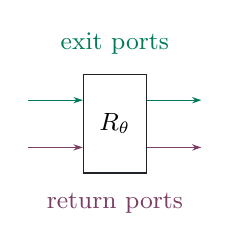
\begin{tikzpicture}[kme circuit,>={Stealth[length=1.2mm,width=.8mm]}]
 \node[kme gate,minimum width=.8cm,minimum height=1.25cm] (r) at
 (1.1,0) {$R_\theta$};
 \draw[flipout,->] (0,.30) -- (r.west |- 0,.30);
 \draw[flipout,->] (r.east |- 0,.30) -- (2.2,.30);
 \draw[flipback,->] (0,-.30) -- (r.west |- 0,-.30);
 \draw[flipback,->] (r.east |- 0,-.30) -- (2.2,-.30);
 \node[text=flipout,above] at (1.1,.80) {exit ports};
 \node[text=flipback,below] at (1.1,-.80) {return ports};
\end{tikzpicture}
\end{minipage}\par

Its type is $(1+1)\leftrightarrow(1+1)$. On input
\code{exit unit}, one call returns
$(3/5)\ket{\mathsf{exit}\,*}+(4/5)\ket{\mathsf{back}\,*}$.
The closing brace ends this definition; it does not feed anything
back. Both payloads are unit, so this example needs no data qubit
beside its guard. Section~\ref{sec:trace} will connect the return
output to the return input.

To evaluate a whole iso, we first replace each checked clause table
$\mathcal T$ by an atom $[M]$ containing its matrix. This gives a
smaller language of \emph{matrix combinators}:
\[
 \kappa::=[M]\mid\kappa;\kappa\mid\kappa\oplus\kappa
                 \mid\kappa\otimes\kappa\mid\kappa^\dagger.
\]
Thus $\omega$ is a source program, $\kappa$ is a program built from
matrix atoms, and $M$ is the matrix computed by that program.

\subsection{Statics}
Match each basis input $s$ against its unique clause and evaluate the
output expression under those bindings. Its vector becomes column $s$
of $M$: entry $M_{ts}$ is the amplitude from input
$s$ to output $t$. Admission requires linearly typed expressions,
a partition of the input basis, equal input and output basis sizes,
and $M^\dagger M=I$. Dagger is conjugate transpose, so the diagonal
entries test squared column norms and the off-diagonal entries test
inner products. Together these make the columns an orthonormal basis.
Figure~\ref{fig:column-test} performs this check on the two clauses
of \code{guardRound}.
\par\begin{figure}[!htbp]\centering
\begin{minipage}{.62\linewidth}\centering
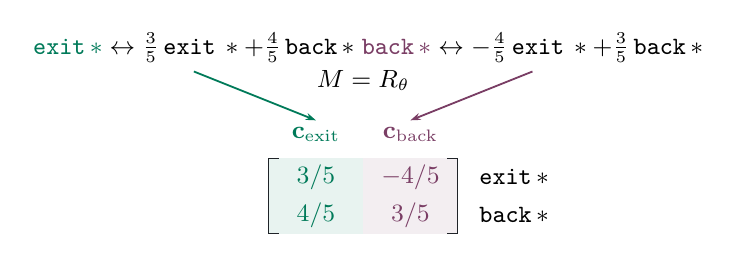
\begin{tikzpicture}[kme circuit,>={Stealth[length=1.3mm,width=.9mm]}]
 \node at (-2.15,1.22)
   {$\textcolor{flipout}{\kw{exit}\,*}\leftrightarrow\tfrac35\,\kw
{exit}\,*+\tfrac45\,\kw{back}\,*$};
 \node at (2.15,1.22)
   {$\textcolor{flipback}{\kw{back}\,*}\leftrightarrow-\tfrac45\,\kw
{exit}\,*+\tfrac35\,\kw{back}\,*$};
 \draw[->,flipout,line width=.65pt] (-2.15,.92) -- (-.60,.30);
 \draw[->,flipback,line width=.65pt] (2.15,.92) -- (.60,.30);
 \node at (0,.80) {$M=R_\theta$};
 \node[text=flipout] at (-.60,.12) {$\mathbf c_{\rm exit}$};
 \node[text=flipback] at (.60,.12) {$\mathbf c_{\rm back}$};
 \fill[flipout!9] (-1.20,-.18) rectangle (0,-1.14);
 \fill[flipback!9] (0,-.18) rectangle (1.20,-1.14);
 \draw[ink] (-1.07,-.18) -- (-1.20,-.18) -- (-1.20,-1.14) --
 (-1.07,-1.14);
 \draw[ink] (1.07,-.18) -- (1.20,-.18) -- (1.20,-1.14) --
 (1.07,-1.14);
 \node[text=flipout] at (-.60,-.42) {$3/5$};
 \node[text=flipout] at (-.60,-.90) {$4/5$};
 \node[text=flipback] at (.60,-.42) {$-4/5$};
 \node[text=flipback] at (.60,-.90) {$3/5$};
 \node[anchor=west] at (1.40,-.42) {\kw{exit}\,$*$};
 \node[anchor=west] at (1.40,-.90) {\kw{back}\,$*$};
\end{tikzpicture}
\end{minipage}\hfill
\begin{minipage}{.35\linewidth}\centering
\begin
{tikzpicture}[x=1.10cm,y=1.10cm,>={Stealth[length=1.3mm,width=.9mm]},
every node/.style={font=\small,inner sep=1pt}]
 \draw[hairline] (0,0) circle (1);
 \draw[muted,->] (-1.08,0) -- (1.14,0);
 \draw[muted,->] (0,-1.08) -- (0,1.14);
 \node[anchor=west] at (1.17,-.09) {$\ket{\kw{exit}\,*}$};
 \node[anchor=south] at (0,1.18) {$\ket{\kw{back}\,*}$};
 \draw[flipout,line width=.9pt,->] (0,0) -- (.6,.8);
 \draw[flipback,line width=.9pt,->] (0,0) -- (-.8,.6);
 \node[text=flipout,anchor=south west] at (.6,.82) {$\mathbf c_{\rm
 exit}$};
 \node[text=flipback,anchor=south east] at (-.8,.62) {$\mathbf c_{\rm
 back}$};
 \draw[ink,line width=.45pt] (.09,.12) -- (-.03,.21) -- (-.12,.09);
\end{tikzpicture}
\end{minipage}
\[
 \|\mathbf c_{\rm exit}\|^2=\frac{9+16}{25}=1,\qquad
 \|\mathbf c_{\rm back}\|^2=\frac{16+9}{25}=1.
\]
\[
 \langle\mathbf c_{\rm exit},\mathbf c_{\rm back}\rangle
=\underbrace{\textcolor{flipout}{\frac35}\,
       \textcolor{flipback}{\left(-\frac45\right)}}_{\text{exit row}}
+\underbrace{\textcolor{flipout}{\frac45}\,
       \textcolor{flipback}{\frac35}}_{\text{back row}}
=-\frac{12}{25}+\frac{12}{25}=0.
\]
\caption{Clauses become colored columns. Their real output vectors
have unit length and zero inner product; the products compare the
same output row. Complex columns use conjugation of the first
factor.}\label{fig:column-test}
\Description{The two source clauses point into green and purple
matrix columns. Those columns are drawn as unit vectors at right
angles and checked by their norms and rowwise inner product.}
\end{figure}\par

The judgment $\Sigma;\Delta\vdash e:b$ uses earlier iso definitions
in $\Sigma$ and variables in the linear context
$\Delta$. Each sum alternative uses the same variables once;
pairs and local applications split disjoint contexts, and result
patterns bind fresh variables. A checked iso has judgment
$\Sigma\vdash\omega:a\leftrightarrow b$. Matrix atoms use the same
column test;
the combinators match their boundary types. A declaration cannot call
itself. It enters $\Sigma$ only after checking. Admission and
evaluation are defined together, recursing only into earlier
definitions or proper subprograms.

The clauses and linear contexts adapt symmetric pattern
matching~\cite[\S\S~3--5]{SabryValironVizzotto18}~\cite
[Ch.~3]{Lemonnier24}.
Appendix~\ref{app:rules} gives the inherited rules in full.

\subsection{Dynamics}
Write $\gamma\vdash e\Downarrow\psi$ for evaluation under a basis
assignment. A value gives
$\ket{v[\gamma]}$ and a sum adds its weighted outputs. A local
application passes every weighted result to its continuation and adds
the resulting vectors, without measurement or normalization.

Elaboration $\mathcal E_\Sigma(\omega)=\kappa$ replaces a checked
table by its atom and unfolds a name in its earlier environment. It
commutes with sequence, sum, tensor and dagger. For $\kappa\Downarrow
M$ and $\lambda\Downarrow N$,
\[
 [M]\Downarrow M,\qquad \kappa;\lambda\Downarrow NM.
\]
Sum, tensor and dagger use the corresponding matrix operations. Write
$\Sigma\vdash\omega\Downarrow M$ when its elaboration evaluates to
$M$. A closed term applies this matrix to its evaluated input vector:
if $t\Downarrow\psi$, then $\omega\,t\Downarrow M\psi$.

\subsection{Denotation}
A type denotes $\sem a=\C^{\mathcal B(a)}$, with its basis values
orthonormal. Thus $0$ and $1$ denote the zero space and
$\C$, and sum and product denote Hilbert sum and tensor. A checked
iso denotes the linear extension of its evaluated columns. The column
check makes this map unitary; Appendix~\ref{app:rules} proves the
interpretation and the inherited combinator cases.

\section{From a round to its exits}\label{sec:trace}
We now add the operation that lets us connect a body's returning
ports and follow an input through the resulting feedback.

\paragraph{Syntax.}
Extend the source and combinator grammars with
$\mathsf{trace}_c\,\omega$ and $\mathsf{trace}_c\,\kappa$,
respectively. Here $\omega$ is a source iso and $\kappa$ is a matrix
combinator program. In either syntax, the constructor connects the
body's output summand of type $c$ to the input summand of the same
type. QWhile uses this typed feedback interface for its do-while
combinator~\cite[\S~5.1]{AndresMartinez22Thesis}.

\paragraph{Statics.}
The external input and output remain after this connection:
\[
 \frac{\Sigma\vdash\beta:a+c\leftrightarrow b+c}
      {\Sigma\vdash\mathsf{trace}_c\,\beta:a\leftrightarrow b}
 \qquad
 \frac{\kappa:a+c\leftrightarrow b+c}
      {\mathsf{trace}_c\,\kappa:a\leftrightarrow b}.
\]
These are typing rules: they specify the remaining input and output
types, without computing the loop. The subscript $c$ is the return
\emph{type}, not a value tag. For a named \kw{round}, the executable
spelling \code{trace f} infers this type from its declaration.
Elaboration preserves the connection:
\[
 \mathcal E_\Sigma(\mathsf{trace}_c\,\omega)
=\mathsf{trace}_c\,\mathcal E_\Sigma(\omega).
\]
\paragraph{Dynamics.}
Let $\beta:a+c\leftrightarrow b+c$ be the source body. Elaboration
gives the matrix program
$\kappa=\mathcal E_\Sigma(\beta)$, and evaluating that program,
$\kappa\Downarrow U$, gives its matrix. For example,
$\code{guardRound}$ elaborates to $[R_\theta]$, which evaluates
to $R_\theta$. The symbol $\kappa$ below always denotes a program.

Put $X=\sem a$, $X'=\sem b$ and $Y=\sem c$. To divide $U$ into four
blocks, group its input columns and output rows by their outer tags.
Evaluating a source input \kw{exit} $s$ supplies the
$A$ and $C$ entries of its column; evaluating \kw{back} $q$
supplies the $B$ and $D$ entries:
\[
\begin{array}{c|cc}
 &\text{input }\mathsf{exit}\ s&\text{input }\mathsf{back}\ q\\
 \hline
 \text{output }\mathsf{exit}\
 t&\textcolor{flipout}{A_{ts}}&\textcolor{flipback}{B_{tq}}\\
 \text{output }\mathsf{back}\
 r&\textcolor{flipout}{C_{rs}}&\textcolor{flipback}{D_{rq}}
\end{array}
\quad
\begin{gathered}
s\in\mathcal B(a),\quad t\in\mathcal B(b),\\ q,r\in\mathcal B(c).
\end{gathered}
\]
Thus $A:X\to X'$ is the immediate external action, $C:X\to Y$ sends
an external input back, $B:Y\to X'$ lets a returning input leave, and
$D:Y\to Y$ sends it back again. On a general vector, these same
entries give
\begin{equation}\label{eq:body-blocks}
U\binom{u}{y}=
 \begin{pmatrix}\textcolor{flipout}{A}&\textcolor{flipback}{B}\\
                 \textcolor{flipout}{C}&\textcolor{flipback}{D}\end
{pmatrix}
 \binom{u}{y}=\binom{Au+By}{Cu+Dy}.
\end{equation}
Here $u\in X$ comes from outside and $y\in Y$ enters on the return
port. The rows give external output $Au+By\in X'$ and returning
output $Cu+Dy\in Y$. The body is \emph{open} because its returning
input and output are still separate ports. Closing them gives the
loop. Unitarity and the common finite $Y$ imply
$\dim X=\dim X'$. For \code{guardRound}, the first clause gives
$A=3/5$ and $C=4/5$; the second gives $B=-4/5$ and $D=3/5$.

The first call on external input $u$ receives $(u,0)$: here $0$ is
absent amplitude on $Y$, not a prepared basis state $\ket0$. Only
$Cu$ supplies the next call, with zero external input.
Figure~\ref{fig:scalar-loop} follows three calls. These are
components of the original amplitude, without normalization; the
block inclusions are ambient linear maps, not reversible gates.
\begin{figure}[!htbp]\centering
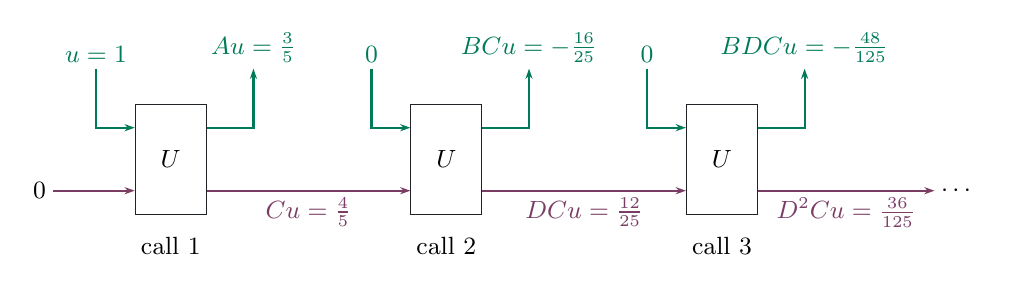
\begin{tikzpicture}[kme circuit,>={Stealth[length=1.3mm,width=.9mm]},
ext/.style={draw=flipout,line width=.8pt},
ret/.style={draw=flipback,line width=.8pt}]
 \foreach \x/\n/\incoming/\emitted in {
1.50/1/{u=1}/{Au=\frac35}, 5.00/2/0/{BCu=-\frac{16}{25}},
8.50/3/0/{BDCu=-\frac{48}{125}}}{
   \node[kme gate,minimum width=.90cm,minimum height=1.40cm] (u\n) at
   (\x,1.10) {$U$};
   \draw[ext,->] (\x-.95,2.25) -- (\x-.95,1.50) -- (u\n.west |-
   0,1.50);
   \node[above,text=flipout] at (\x-.95,2.25) {$\incoming$};
   \draw[ext,->] (u\n.east |- 0,1.50) -- (\x+1.05,1.50) --
   (\x+1.05,2.25);
   \node[above,text=flipout] at (\x+1.05,2.25) {$\emitted$};
   \node at (\x,.00) {call \n};
 }
 \draw[ret,->] (.00,.70) node[left] {$0$} -- (u1.west |- 0,.70);
 \draw[ret,->] (u1.east |- 0,.70)
-- node[below,text=flipback] {$Cu=\frac45$} (u2.west |- 0,.70);
 \draw[ret,->] (u2.east |- 0,.70)
-- node[below,text=flipback] {$DCu=\frac{12}{25}$} (u3.west |-
0,.70);
 \draw[ret,->] (u3.east |- 0,.70)
-- node[below,text=flipback] {$D^2Cu=\frac{36}{125}$} (11.20,.70);
 \node at (11.50,.70) {$\cdots$};
\end{tikzpicture}
\caption{Three calls, with scalar values for $U=R_\theta$ and $u=1$.
Purple return components alone supply the next call; later external
inputs have zero amplitude.}\label{fig:scalar-loop}
\Description{Three complete two-port bodies show general block
formulas and the corresponding scalar amplitudes. Successive exits
are three fifths, minus sixteen twenty-fifths and minus forty-eight
one-hundred-and-twenty-fifths. The third return is thirty-six
one-hundred-and-twenty-fifths and continues.}
\end{figure}

Define $x_k:X\to X'$ to be the exit map after $k$ returns. Thus count
$k$ means $k+1$ body calls, including the first; adding one to the
label gives the number of iterations from the introduction. The
immediate exit is $A$. To exit after $k+1$ returns, a contribution
first enters $Y$ through $C$, makes $k$ further passages through $D$,
and finally leaves through $B$. Its exit maps are therefore
\begin{equation}\label{eq:exits}
x_0=A,\qquad x_{k+1}=BD^kC.
\end{equation}
After $n+1$ calls, the emissions are $x_0u,\ldots,x_nu$ and the
remainder is $D^nCu$. The three loop readings differ in how they
combine this same exit sequence.

Closing the return port identifies its outgoing vector $Cu+Dy$ with
its incoming vector $y$. Thus, for external input $u$, the connected
wire must satisfy $y=Cu+Dy$. We call this the
\emph{wire equation}. Any solution gives external output $Au+By$.

The evaluator must compute the whole closed matrix, so it solves this
equation on each external basis input $s$. Let $y_s$ be a solution of
the finite linear system $(I_Y-D)y_s=C\ket s$. The corresponding
output column is $A\ket s+By_s$. Collecting the returning columns
into a map $F:X\to Y$, with $F\ket s=y_s$, gives $(I_Y-D)F=C$ and
output matrix $A+BF$. The rule first evaluates the open program, then
solves its returning columns:
\[
 \frac{\kappa\Downarrow U\quad
U=\left(\begin{smallmatrix}A&B\\C&D\end{smallmatrix}\right)
       \quad F:X\to Y\quad (I_Y-D)F=C}
      {\mathsf{trace}_c\,\kappa\Downarrow A+BF}.
\]
Applied to input $u$, the closed matrix $A+BF$ returns $(A+BF)u$ at
type $b$, with the return summand removed. The earlier typing rules
specify its boundary; this rule computes its action.

Theorem~\ref{thm:total} proves that a solution exists whenever the
well-typed body $\kappa$ evaluates to a finite unitary $U$. The
matrix $I_Y-D$ may be singular, meaning it has no inverse. In that
case two wire solutions can differ, but their difference
$v$ satisfies $Dv=v$. Unitarity then forces $Bv=0$: a returning
vector that preserves all its norm internally cannot also emit norm
through $B$. Thus all solutions give the same external output, and
the rule still determines one matrix.

To depict this connection, we use \emph{sheet diagrams}, read
upwards. Separate sheets carry sum alternatives, whereas wires at
different depths on one sheet carry tensor factors~\cite[Defs.~16,
18--20]{ComfortDelpeuchHedges20Sheets}. The circled $U$ at a seam
acts on both incident summands; a sheet in front may hide part of the
other wire, but does not remove it. In Figure~\ref{fig:28-sheets},
bending the $Y$ sheet back to that seam connects its output to its
input.
\begin{programfigure}
\begin{minipage}{.70\linewidth}\centering
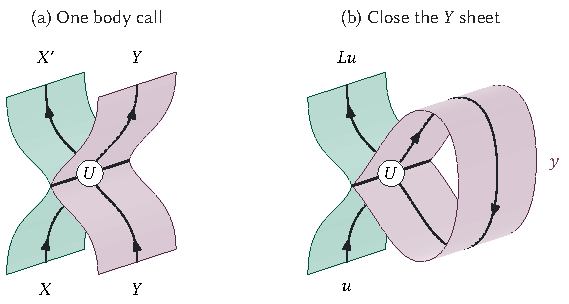
\includegraphics{figures/28-sheets.pdf}
\end{minipage}\hfill
\begin{minipage}{.27\linewidth}\raggedright
Closing the return gives
\[
 \begin{aligned}
y&=Cu+Dy,\\ Lu&=Au+By.
 \end{aligned}
\]
For the atom $[R_\theta]$,
\[
 \begin{gathered}
(1-\tfrac35)F=\tfrac45,\\ F=2,\\
 \tfrac35-\tfrac45 F=-1,\\
 \mathsf{trace}_1[R_\theta]\Downarrow(-1).
 \end{gathered}
\]
\end{minipage}
\caption{Direct-sum feedback identifies the two ends of the returning
$Y$ sheet. The annotations evaluate the rotation by the trace
rule.}\label{fig:28-sheets}
\Description{Separate sheets carry the external and returning
summands. The returning sheet bends back to the same body. Equations
beside the drawing identify its input and output amplitudes and
calculate the scalar instance.}
\end{programfigure}
For the rotation, elaboration supplies the atom $[R_\theta]$.
Figure~\ref{fig:28-sheets} solves its returning column, giving
$F=2$ and closed matrix $(-1)$. The returning value $2$ is a sum
of amplitudes, rather than a normalized state on a new register. The
computed closed iso is
$\{*\leftrightarrow-1\cdot *\}:1\leftrightarrow1$, so
\[
 \code{trace guardRound on unit}\Downarrow-\ket*.
\]
The closing operation removes both port tags and returns a value of
type $1$. A single call to the open \code{guardRound} still returns
its tagged superposition from the first column.

\paragraph{Denotation.}
Coherent feedback adds all the emissions on their common external
output:
\[
 \sem{\mathsf{trace}_c\,\beta}=L=\sum_{k\ge0}x_k.
\]
This is the established direct-sum execution
formula~\cite{AbramskyHaghverdiScott02GoI}. Theorem~\ref{thm:total}
identifies it with the wire-equation output, so the operational rule
and categorical trace $\Tr^Y(U)$ compute the same map.

\paragraph{Why is the sum defined for every finite body?}
For a finite unitary body, the established feedback theorem gives
absolute convergence of the exits, a unitary sum $L$, and
$\sum_kx_k^\dagger x_k=I_X$~\cite[Thms.~4, 7,
8]{Bartha14QuantumTuringAutomata}~\cite[Thm.~3.3.15,
Cor.~3.3.16]{AndresMartinez22Thesis}. Its proof separates the
internal vectors that never emit from those that do. Unitarity
prevents the external input from entering that closed component; on
the emitting part the returns decay geometrically.
Appendix~\ref{app:total} proves this by the norm accounting in
Figure~\ref{fig:feedback-proof}. No last nonzero exit is required.

\par\noindent\begin{minipage}{.70\linewidth}
Take $U=R_\theta\oplus1$, with ordered coordinates $(u,y_0,y_1)$.
Here $y_0$ is the emitting return and $y_1$ is the isolated one.
Connecting these two return ports gives
\[
 \tfrac25y_0=\tfrac45u,\qquad y_1=y_1,\qquad y_0=2u.
\]
\end{minipage}\hfill
\begin{minipage}{.27\linewidth}\centering
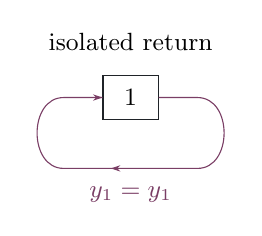
\begin{tikzpicture}[kme circuit,>={Stealth[length=1.2mm,width=.8mm]}]
 \node[kme gate] (d) at (0,.45) {$1$};
 \draw[flipback] (d.east) -- (.85,.45)
.. controls (1.30,.45) and (1.30,-.45) .. (.85,-.45) -- (-.85,-.45)
.. controls (-1.30,-.45) and (-1.30,.45) .. (-.85,.45) -- (d.west);
 \draw[flipback,->] (-.85,.45) -- (d.west);
 \draw[flipback,->] (.25,-.45) -- (-.25,-.45);
 \node[above] at (0,.97) {isolated return};
 \node[below,text=flipback] at (0,-.61) {$y_1=y_1$};
\end{tikzpicture}
\end{minipage}\par
The isolated amplitude $y_1$ is arbitrary, but only $y_0$ enters the
output $(3/5)u-(4/5)y_0=-u$. Thus
$D=\operatorname{diag}(3/5,1)$ makes $I_Y-D$ singular without
making the loop's output ambiguous. For rotations approaching the
identity the loop remains $-1$, but at the identity it is
$+1$~\cite[Remark~B.1]{FairbanksSelinger25Traces}.

\paragraph{Computing the closed iso.}
The wire equation $y=Cu+Dy$ asks which amplitude must enter each
return pattern when its output is connected back to its input. For a
basis value $q\in\mathcal B(c)$, $y_q=\langle q|y\rangle$ is the
amplitude on \kw{back} $q$. The entry $D_{qq}$ is the coefficient of
\kw{back} $q$ in the ground clause whose input is also \kw{back} $q$.
For \code{guardRound}, $q=*$ and
$D_{qq}=3/5$. The coordinate equation is
\[
(1-D_{qq})y_q=(Cu)_q+\sum_{r\ne q}D_{qr}y_r.
\]
If $D_{qq}\ne1$, divide by $1-D_{qq}$ and substitute for $y_q$ in the
other return equations and the external output $v=Au+By$. In the
ground clause table, this removes the input pattern
\kw{back} $q$ and replaces every output occurrence of that pattern
by the other terms of its clause, scaled by $1/(1-D_{qq})$.
Coefficients multiply along a substituted path and add when paths
reach the same output. If $D_{qq}=1$, unitarity forces every other
entry in that row and column to vanish, so the isolated pattern can
simply be removed. The smaller body is again unitary. Repeating with
its updated coefficients eventually leaves only external clauses.
Removing their \kw{exit} tags gives the atom
$[L]:a\leftrightarrow b$ with output $v=Lu$.
This is the established elimination for finite contractions,
including unitaries~\cite[Thm.~3.3.15]{AndresMartinez22Thesis};
Appendix~\ref{app:elim} proves order independence and preservation of
the coefficient subfield.

Figure~\ref{fig:42-elim-flip} follows two such steps for
\code{flipRound}, whose body $\beta_{\rm flip}$ rotates the guard
as before and flips a data bit on each call. Here $u_0,u_1$ are the
input amplitudes on \kw{exit} $0,1$, $y_0,y_1$ are the returning
amplitudes on \kw{back} $0,1$, and $v_0,v_1$ are the external output
amplitudes. Substituting for $y_0$ creates a self-coefficient $9/25$
on the remaining return $y_1$. Solving that wire equation and
substituting into the outputs gives $v=-u$. Appendix~\ref{app:flip}
gives the iso clauses.
\begin{figure}[!htbp]\centering
\begingroup
\newcommand{\elimret}[1]{\textcolor{flipback}{#1}}
\newcommand{\elimext}[1]{\textcolor{flipout}{#1}}
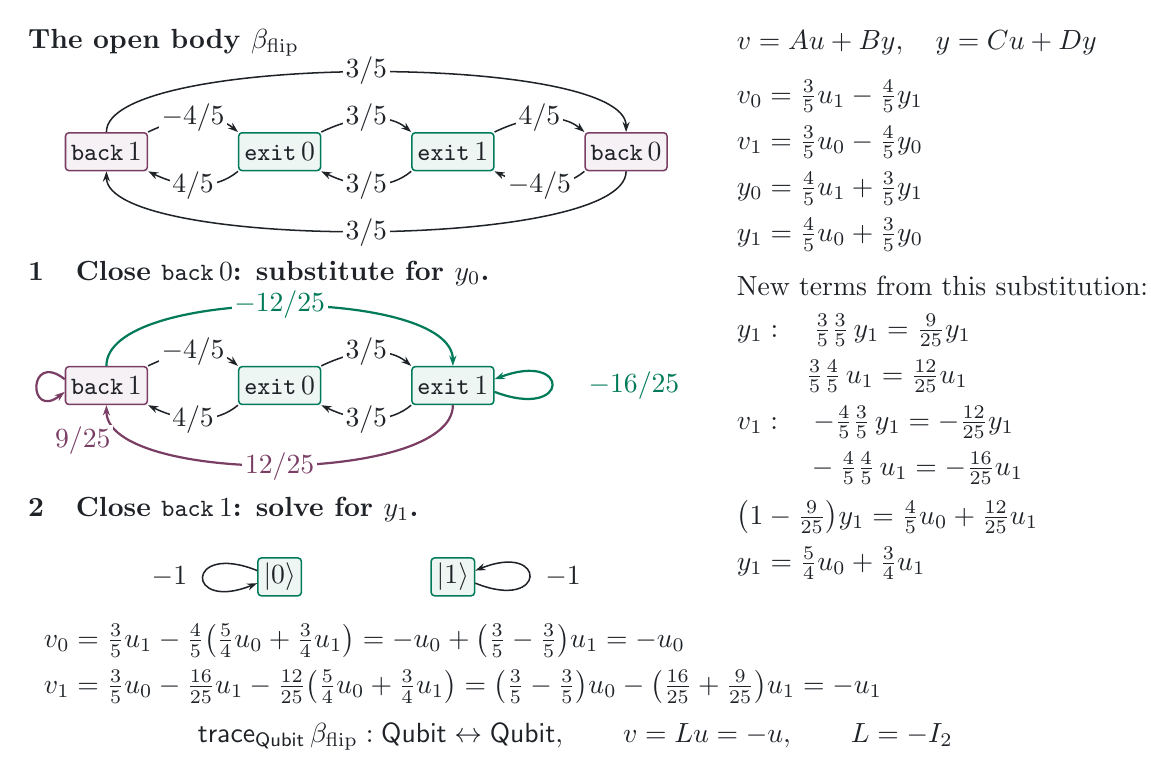
\begin{tikzpicture}[x=1mm,y=.90mm,
>={Stealth[length=1.3mm,width=.9mm]}, every
node/.style={font=\fontsize{9.8}{12}\selectfont,text=ink,inner
sep=0pt}, elim/tag/.style={draw,line width=.55pt,rounded
corners=1.2pt, minimum height=4.8mm,inner xsep=2pt,inner ysep=1.2pt},
elim/exit/.style={elim/tag,draw=flipout,fill=flipout!7},
elim/back/.style={elim/tag,draw=flipback,fill=flipback!7},
elim/flow/.style={draw=ink,line width=.55pt,->},
elim/weight/.style={fill=white,inner xsep=1pt,inner ysep=.6pt},
elim/head/.style={anchor=west,font=\fontsize{9.8}{12}\selectfont
\bfseries},
elim/eq/.style={anchor=west}]
\path[use as bounding box] (0,0) rectangle (139.1,101.5);

\node[elim/head] at (0,99.4) {The open body $\beta_{\rm flip}$};
\node[elim/eq] at (90,99.4) {$v=Au+By,\quad y=Cu+Dy$};
\begin{scope}[shift={(0,84)}]
\node[elim/back] (a-b1) at (10,0) {\kw{back}\,$1$};
\node[elim/exit] (a-e0) at (32,0) {\kw{exit}\,$0$};
\node[elim/exit] (a-e1) at (54,0) {\kw{exit}\,$1$};
\node[elim/back] (a-b0) at (76,0) {\kw{back}\,$0$};
\draw[elim/flow] (a-b1.north east) .. controls (20,5.3) and (24,5.3)
.. (a-e0.north west);
\node[elim/weight] at (21,4.8) {$-4/5$};
\draw[elim/flow] (a-e0.south west) .. controls (24,-5.3) and
(20,-5.3) .. (a-b1.south east);
\node[elim/weight] at (21,-4.8) {$4/5$};
\draw[elim/flow] (a-e0.north east) .. controls (42,5.3) and (46,5.3)
.. (a-e1.north west);
\node[elim/weight] at (43,4.8) {$3/5$};
\draw[elim/flow] (a-e1.south west) .. controls (46,-5.3) and
(42,-5.3) .. (a-e0.south east);
\node[elim/weight] at (43,-4.8) {$3/5$};
\draw[elim/flow] (a-e1.north east) .. controls (64,5.3) and (68,5.3)
.. (a-b0.north west);
\node[elim/weight] at (65,4.8) {$4/5$};
\draw[elim/flow] (a-b0.south west) .. controls (68,-5.3) and
(64,-5.3) .. (a-e1.south east);
\node[elim/weight] at (65,-4.8) {$-4/5$};
\draw[elim/flow] (a-b1.north) .. controls (10,14) and (76,14) ..
(a-b0.north);
\node[elim/weight] at (43,11.4) {$3/5$};
\draw[elim/flow] (a-b0.south) .. controls (76,-14) and (10,-14) ..
(a-b1.south);
\node[elim/weight] at (43,-11.4) {$3/5$};
\end{scope}
\node[elim/eq] at (90,91.8)
{$\elimext{v_0}=\tfrac35u_1-\tfrac45\elimret{y_1}$};
\node[elim/eq] at (90,85.3)
{$\elimext{v_1}=\tfrac35u_0-\tfrac45\elimret{y_0}$};
\node[elim/eq] at (90,78.8)
{$\elimret{y_0}=\tfrac45u_1+\tfrac35\elimret{y_1}$};
\node[elim/eq] at (90,72.3)
{$\elimret{y_1}=\tfrac45u_0+\tfrac35\elimret{y_0}$};

\node[elim/head] at (0,66.8) {1\quad Close \kw{back}\,$0$: substitute
for $\elimret{y_0}$.};
\node[elim/eq] at (90,65.1) {New terms from this substitution:};
\begin{scope}[shift={(0,51)}]
\node[elim/back] (b-b1) at (10,0) {\kw{back}\,$1$};
\node[elim/exit] (b-e0) at (32,0) {\kw{exit}\,$0$};
\node[elim/exit] (b-e1) at (54,0) {\kw{exit}\,$1$};
\draw[elim/flow] (b-b1.north east) .. controls (20,5.3) and (24,5.3)
.. (b-e0.north west);
\node[elim/weight] at (21,4.8) {$-4/5$};
\draw[elim/flow] (b-e0.south west) .. controls (24,-5.3) and
(20,-5.3) .. (b-b1.south east);
\node[elim/weight] at (21,-4.8) {$4/5$};
\draw[elim/flow] (b-e0.north east) .. controls (42,5.3) and (46,5.3)
.. (b-e1.north west);
\node[elim/weight] at (43,4.8) {$3/5$};
\draw[elim/flow] (b-e1.south west) .. controls (46,-5.3) and
(42,-5.3) .. (b-e0.south east);
\node[elim/weight] at (43,-4.8) {$3/5$};
\draw[elim/flow,draw=flipout,line width=.8pt] (b-b1.north) ..
controls (10,14) and (54,14) .. (b-e1.north);
\node[elim/weight,text=flipout] at (32,11.4) {$-12/25$};
\draw[elim/flow,draw=flipback,line width=.8pt] (b-e1.south) ..
controls (54,-14) and (10,-14) .. (b-b1.south);
\node[elim/weight,text=flipback] at (32,-11.4) {$12/25$};
\draw[elim/flow,draw=flipback,line width=.8pt]
([yshift=.8mm]b-b1.west)
.. controls (0,5) and (0,-5) .. ([yshift=-.8mm]b-b1.west);
\node[elim/weight,text=flipback] at (7,-7.8) {$9/25$};
\draw[elim/flow,draw=flipout,line width=.8pt]
([yshift=-.8mm]b-e1.east)
.. controls (69,-5) and (69,5) .. ([yshift=.8mm]b-e1.east);
\node[elim/weight,text=flipout] at (77,0) {$-16/25$};
\end{scope}
\node[elim/eq] at (90,58.8) {$\elimret{y_1}:\quad
\tfrac35\tfrac35\,y_1=\tfrac9{25}y_1$};
\node[elim/eq] at (90,52.3) {$\phantom{y_1:}\quad
\tfrac35\tfrac45\,u_1=\tfrac{12}{25}u_1$};
\node[elim/eq] at (90,45.8) {$\elimext{v_1}:\quad
-\tfrac45\tfrac35\,y_1=-\tfrac{12}{25}y_1$};
\node[elim/eq] at (90,39.3) {$\phantom{v_1:}\quad
-\tfrac45\tfrac45\,u_1=-\tfrac{16}{25}u_1$};

\node[elim/head] at (0,33.5) {2\quad Close \kw{back}\,$1$: solve for
$\elimret{y_1}$.};
\node[elim/eq] at (90,32.4)
 {$\bigl(1-\tfrac9{25}\bigr)y_1=\tfrac45u_0+\tfrac{12}{25}u_1$};
\node[elim/eq] at (90,25.9)
{$\elimret{y_1}=\tfrac54u_0+\tfrac34u_1$};
\begin{scope}[shift={(0,24)}]
\node[elim/exit] (c-e0) at (32,0) {$\ket0$};
\node[elim/exit] (c-e1) at (54,0) {$\ket1$};
\draw[elim/flow] ([yshift=.8mm]c-e0.west)
.. controls (20,5) and (20,-5) .. ([yshift=-.8mm]c-e0.west);
\node[elim/weight] at (18,0) {$-1$};
\draw[elim/flow] ([yshift=-.8mm]c-e1.east)
.. controls (66,-5) and (66,5) .. ([yshift=.8mm]c-e1.east);
\node[elim/weight] at (68,0) {$-1$};
\end{scope}
\node[elim/eq] at (2,15)
 {$\elimext{v_0}=\tfrac35u_1-\tfrac45\bigl(\tfrac54u_0+\tfrac
34u_1\bigr)
=-u_0+\bigl(\tfrac35-\tfrac35\bigr)u_1=\elimext{-u_0}$};
\node[elim/eq] at (2,8.5)
 {$\elimext{v_1}=\tfrac35u_0-\tfrac{16}{25}u_1-\tfrac{12}{25}\bigl
(\tfrac54u_0+\tfrac34u_1\bigr)
=\bigl(\tfrac35-\tfrac35\bigr)u_0-\bigl(\tfrac{16}{25}+\tfrac
9{25}\bigr)u_1
=\elimext{-u_1}$};
\node at (69.55,1.4)
 {$\mathsf{trace}_{\mathsf{Qubit}}\,\beta_{\rm
 flip}:\mathsf{Qubit}\leftrightarrow\mathsf{Qubit},
    \qquad v=Lu=-u,\qquad L=-I_2$};
\end{tikzpicture}
\endgroup
\caption{Eliminating the two returns of \code{flipRound}. An arrow
gives an amplitude from its input port to its output port. The
colored arrows in the middle graph are created by substituting for
$y_0$; their products are at right. Solving the remaining equation
gives the untagged output $v=-u$.}\label{fig:42-elim-flip}
\Description{Three stacked port graphs show the original four ports,
the three ports after closing back zero, and the two untagged
external ports after closing back one. The component wire equations
and all changed coefficients are beside the corresponding graph; both
external-output cancellations are calculated below.}
\end{figure}
\FloatBarrier

\paragraph{The rotation and its reference.}
For \code{guardRound}, put $t=3/5$ and $s=4/5$, so
$A=D=t$, $C=s$ and $B=-s$. On input $\ket*$, the first call
emits amplitude $t$ and sends amplitude $s$ back. Let $r_n$ be the
amplitude still returning after call $n$, with $r_1=s$. The next call
sends $-sr_n$ out and $tr_n$ back. Coherent feedback adds the new
emission to the sum $\ell_n$ of all earlier emissions. If the guard
is measured on each call, we instead add the squared magnitude of
that emission to the cumulative halting probability $p_n$. Starting
with $\ell_1=t$ and $p_1=t^2$, these updates are
\[
r_{n+1}=tr_n,\qquad \ell_{n+1}=\ell_n-sr_n,\qquad
p_{n+1}=p_n+s^2|r_n|^2.
\]
Table~\ref{tab:rounds} separates the two calculations. The coherent
sum can shrink through cancellation, while $p_n$ only increases.
Section~\ref{sec:effects} defines the recording and measured loops.
\begin{table}[!htbp]\centering
\small
\begin{tabular}{c r r r r r}
\toprule
 & \multicolumn{2}{c}{one call}
 & \multicolumn{2}{c}{coherent feedback}
 & guard measured\\
\cmidrule(lr){2-3}\cmidrule(lr){4-5}\cmidrule(l){6-6}
call $n$ & \shortstack{emitted\\$x_{n-1}$}
 & \shortstack{still returning\\$r_n$}
 & \shortstack{sum emitted\\$\ell_n$}
 & \shortstack{squared length\\$|\ell_n|^2$}
 & \shortstack{halted so far\\$p_n$}\\
\midrule
1 & $\textcolor{flipout}{\tfrac35}$
  & $\textcolor{flipback}{\tfrac45}$ & $\tfrac35$ & $0.3600$
  & $\textcolor{accentwarm}{0.3600}$\\[3pt]
2 & $\textcolor{flipout}{-\tfrac{16}{25}}$
  & $\textcolor{flipback}{\tfrac{12}{25}}$ & $-\tfrac1{25}$ &
  $0.0016$
  & $\textcolor{accentwarm}{0.7696}$\\[3pt]
3 & $\textcolor{flipout}{-\tfrac{48}{125}}$
  & $\textcolor{flipback}{\tfrac{36}{125}}$ & $-\tfrac{53}{125}$ &
  $0.1798$
  & $\textcolor{accentwarm}{0.9171}$\\[3pt]
4 & $\textcolor{flipout}{-\tfrac{144}{625}}$
  & $\textcolor{flipback}{\tfrac{108}{625}}$ & $-\tfrac{409}{625}$ &
  $0.4282$
  & $\textcolor{accentwarm}{0.9701}$\\[3pt]
5 & $\textcolor{flipout}{-\tfrac{432}{3125}}$
  & $\textcolor{flipback}{\tfrac{324}{3125}}$ & $-\tfrac{2477}{3125}$
  & $0.6283$
  & $\textcolor{accentwarm}{0.9893}$\\[3pt]
$n\to\infty$ & $0$ & $0$ & $-1$ & $1$ & $1$\\
\bottomrule
\end{tabular}
\caption{\code{guardRound} on $\ket*$. Coherent feedback adds
emissions, while guard measurement adds their squared magnitudes. A
record keeps emission $x_{n-1}$ with label $n-1$. Only $p_n$ is a
halting probability; decimal entries are rounded to four
places.}\label{tab:rounds}
\end{table}

In the limit $\ell_n\to-1$ and $p_n\to1$, so both readings return the
only external value $*$ with certainty. The coherent phase $-\ket*$
is global on this interface. To observe it, we place the loop beside
an unaffected amplitude.

\Needspace{9\baselineskip}
Add the bypass by changing the external type to $\kw{Qubit}=1+1$,
with $0$ for the bypass and $1$ for the loop arm. Keep the return
type \kw{Unit}, leave external $0$ unchanged, and rotate external
$1$ with the return port:
\begin{lstlisting}
round withReference : Qubit + Unit = {
  exit 0 <-> exit 0;
  exit 1 <-> [ 3/5 . exit 1 + 4/5 . back unit];
  back unit <-> [-4/5 . exit 1 + 3/5 . back unit]
}
\end{lstlisting}
Use \code{exit 0}, \code{exit 1}, \code{back unit} as the ordered
input and output bases. The three clauses give the three columns
below. The first two rows and columns belong to the external qubit,
and the last row and column belong to the return port. The boxed
letters name the four blocks of~\eqref{eq:body-blocks}.
\begin{center}
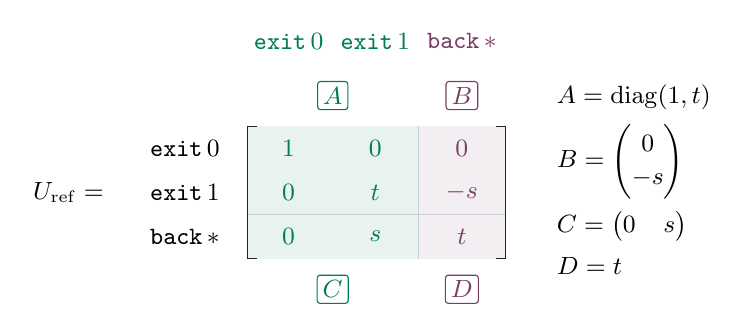
\begin{tikzpicture}[kme circuit,
blockname/.style={draw,rounded corners=1pt,fill=white,inner sep=2pt}]
 \node[text=flipout] at (.52,1.92) {\kw{exit}\,$0$};
 \node[text=flipout] at (1.62,1.92) {\kw{exit}\,$1$};
 \node[text=flipback] at (2.72,1.92) {\kw{back}\,$*$};
 \node[anchor=east] at (-.28,.56) {\kw{exit}\,$0$};
 \node[anchor=east] at (-.28,0) {\kw{exit}\,$1$};
 \node[anchor=east] at (-.28,-.56) {\kw{back}\,$*$};
 \node[anchor=east] at (-1.75,0) {$U_{\rm ref}=$};
 \fill[flipout!9] (0,-.84) rectangle (2.17,.84);
 \fill[flipback!9] (2.17,-.84) rectangle (3.27,.84);
 \draw[ink] (.12,.84) -- (0,.84) -- (0,-.84) -- (.12,-.84);
 \draw[ink] (3.15,.84) -- (3.27,.84) -- (3.27,-.84) -- (3.15,-.84);
 \draw[hairline] (2.17,-.84) -- (2.17,.84);
 \draw[hairline] (0,-.28) -- (3.27,-.28);
 \foreach \x/\y/\entry in
 {.52/.56/1,1.62/.56/0,.52/0/0,1.62/0/t,.52/-.56/0,1.62/-.56/s}
   \node[text=flipout] at (\x,\y) {$\entry$};
 \foreach \y/\entry in {.56/0,0/{-s},-.56/t}
   \node[text=flipback] at (2.72,\y) {$\entry$};
 \node[blockname,draw=flipout,text=flipout] at (1.08,1.23) {$A$};
 \node[blockname,draw=flipback,text=flipback] at (2.72,1.23) {$B$};
 \node[blockname,draw=flipout,text=flipout] at (1.08,-1.23) {$C$};
 \node[blockname,draw=flipback,text=flipback] at (2.72,-1.23) {$D$};
 \node[anchor=west,align=left] at (3.85,.64)
   {$A=\operatorname{diag}(1,t)$\\[4pt]$B=\displaystyle\binom0{-s}$};
 \node[anchor=west,align=left] at (3.85,-.64)
   {$C=\begin{pmatrix}0&s\end{pmatrix}$\\[4pt]$D=t$};
\end{tikzpicture}
\end{center}
Substituting these blocks into the exit formula gives
\[
x_0=\operatorname{diag}(1,t),\qquad
x_{k+1}=\binom0{-s}\,t^k\begin{pmatrix}0&s\end{pmatrix}
=\begin{pmatrix}0&0\\0&-s^2t^k\end{pmatrix}.
\]
Only the immediate exit contains the bypass. Summing the lower right
entries gives $-1$ as before, so the closed gate is
$L=\operatorname{diag}(1,-1)$ on the external qubit. Finite
elimination gives the same external clauses:
$\{0\leftrightarrow0,\ 1\leftrightarrow-1\cdot1\}$.

The standard \emph{Hadamard test} makes this relative phase
observable~\cite[p.~1, Eqs.~(1)--(3)]{Childs13Hadamard}. Its Hadamard
iso has two clauses, one for each input column:
\[
H=\{0\leftrightarrow\tfrac1{\sqrt2}(0+1),\quad
1\leftrightarrow\tfrac1{\sqrt2}(0-1)\}
:\kw{Qubit}\leftrightarrow\kw{Qubit},\qquad
 \sem H=\frac1{\sqrt2}\begin{pmatrix}1&1\\1&-1\end{pmatrix}.
\]
It sends input $\ket0$ to
$\ket+=(\ket0+\ket1)/\sqrt2$, supplying amplitude to both arms.
The coherent loop changes this to
$\ket-=(\ket0-\ket1)/\sqrt2$. Applying $H$ again gives
$\ket1$, so a computational-basis measurement returns $1$
with certainty. The composition
$H;\mathsf{trace}_1\,\mathsf{withReference};H$
uses the Hadamard iso just defined on both sides of the closed body.
Here the controlled operation is just the scalar loop, so the control
qubit is the entire external data. Figure~\ref{fig:bypass-intro}
shows the test and expands its two arms. Section~\ref{sec:effects}
will run the same test after measuring the loop's return tag and
obtain probability $1/5$ for outcome $1$.
\begin{figure}[!htbp]\centering
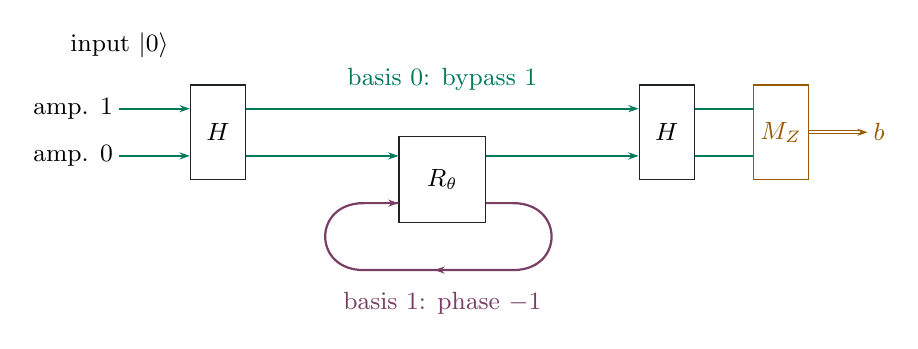
\begin{tikzpicture}[kme circuit,>={Stealth[length=1.3mm,width=.9mm]},
pass/.style={draw=flipout,line width=.8pt},
ret/.style={draw=flipback,line width=.8pt}]
 \node[anchor=west] at (-.55,2.00) {input $\ket0$};
 \node[kme gate,minimum height=1.20cm] (h1) at (1.40,.90) {$H$};
 \draw[pass,->] (.15,1.20) node[left] {amp. $1$} -- (h1.west |-
 0,1.20);
 \draw[pass,->] (.15,.60) node[left] {amp. $0$} -- (h1.west |-
 0,.60);
 \node[kme gate,minimum width=1.10cm,minimum height=1.10cm] (u) at
 (4.25,.30) {$R_\theta$};
 \node[kme gate,minimum height=1.20cm] (h2) at (7.10,.90) {$H$};
 \draw[pass,->] (h1.east |- 0,1.20) -- (h2.west |- 0,1.20);
 \node[above,text=flipout] at (4.25,1.35) {basis $0$: bypass $1$};
 \draw[pass,->] (h1.east |- 0,.60) -- (u.west |- 0,.60);
 \draw[pass,->] (u.east |- 0,.60) -- (h2.west |- 0,.60);
 \node[below,text=flipback] at (4.25,-1.06) {basis $1$: phase $-1$};
 \draw[ret] (u.east |- 0,0) -- (5.15,0)
.. controls (5.80,0) and (5.80,-.85) .. (5.15,-.85) -- (3.25,-.85) ..
controls (2.60,-.85) and (2.60,0) .. (3.25,0) -- (u.west |- 0,0);
 \draw[ret,->] (3.25,0) -- (u.west |- 0,0);
 \draw[ret,->] (4.65,-.85) -- (4.15,-.85);
 \node[kme gate,draw=accentwarm,text=accentwarm,minimum
 height=1.20cm] (m) at (8.55,.90) {$M_Z$};
 \draw[pass] (h2.east |- 0,1.20) -- (m.west |- 0,1.20);
 \draw[pass] (h2.east |- 0,.60) -- (m.west |- 0,.60);
 \draw[accentwarm,double,double distance=.65pt,->] (m.east) --
 (9.65,.90) node[right] {$b$};
\end{tikzpicture}
\caption{The two rails are the basis alternatives of
$\kw{Qubit}=1+1$. Only basis $1$ enters the scalar loop, whose
rotation has $\cos\theta=t=3/5$. The second $H$ recombines its phase
with the bypass, giving $b=1$ with
certainty.}\label{fig:bypass-intro}
\Description{Two-port Hadamard couplers place the scalar rotation
feedback loop beside a bypass and recombine their amplitudes before a
computational-basis measurement. The initial amplitudes are one and
zero.}
\end{figure}

Elimination computes $L$ without retaining its decomposition into
exits. To compare feedback with measurement, we now keep that
decomposition: attach a count label to each $x_ku$, discard those
labels and compare the returned data with $Lu$.

\FloatBarrier
\section{What allocation and hiding do to the
loop}\label{sec:effects}
Returning a count requires a register the caller did not supply.
Following \emph{Quantum Information Effects}, allocation exposes an
input summand of a unitary and hiding discards an output factor of an
isometry~\cite[\S\S~3--4, Thm.~22]{HeunenKaarsgaard22Effects}. These
extend finite iso first to $\mathsf{iso}_a$ isometries, then to
$\mathsf{iso}_a^\chi$ channels. We need both extensions to carry out
the classical idea from the introduction: allocation supplies the
count register, and hiding lets the caller ignore it. Together they
also derive measurement, which will distinguish exit from return
inside every call.

\paragraph{Syntax.}
An allocation program $v:a\rightarrowtail b$ is built from
$\mathsf{arr}\,\omega$, $\mathsf{lift}\,\omega$, sequence,
sum and tensor; a channel program $h:a\rightsquigarrow b$ uses
$\mathsf{arr}\,v$, $\mathsf{hide}\,v$, sequence and tensor.
We add the forms $\mathsf{count}_K\,\omega$ and
$\mathsf{while}_c\,\omega$, with $K\ge1$ and a reversible body.
Their definitions follow below; the full grammars and inherited rules
are in Appendix~\ref{app:rules}. The executable spelling \code{while
f} infers $c$ from a named
\kw{round}, as \code{trace f} does.

\paragraph{Statics.}
An embedding $\mathsf{arr}$ retains its program's input and output
types. Given $\omega:a+d\leftrightarrow b$, allocation produces
$\mathsf{lift}\,\omega:a\rightarrowtail b$ by selecting the $a$
input summand. Given $v:a\rightarrowtail b\otimes g$ with
$\mathcal B(g)\ne\varnothing$, hiding produces
$\mathsf{hide}\,v:a\rightsquigarrow b$ by removing the $g$ factor.
The loop rules, with their common environment $\Sigma$ omitted, are
\begin{mathpar}
 \isorule{\beta:a+c\leftrightarrow b+c\\K\ge1}
         {\mathsf{count}_K\,\beta:a\rightarrowtail[K]\otimes b}
 \and\isorule{\beta:a+c\leftrightarrow b+c}
         {\mathsf{while}_c\,\beta:a\rightsquigarrow b}.
\end{mathpar}
Sequence matches intermediate types, while tensor forms products of
input and of output types. Isometries also combine by direct sum,
while channels have no coherent sum constructor. The type $[K]$ is
the $K$-fold sum of $1$, with basis labels $0,\ldots,K-1$.

\paragraph{Dynamics.}
If $\omega\Downarrow U$, evaluating $\mathsf{lift}\,\omega$ uses only
the input columns belonging to $a$, so input $u$ gives
$U(u,0)$. If $v\Downarrow V$, evaluating $\mathsf{hide}\,v$ on
a density operator $\rho$ gives $\tr_g(V\rho V^\dagger)$. Here a
density operator is a positive semidefinite matrix of trace one; a
unit vector $u$ has state $\ket u\bra u$. The partial trace sums
diagonal blocks indexed by the hidden factor's basis. The first
$\mathsf{arr}$ retains the unitary matrix, while the second sends an
isometry $V$ to
$\chan V:\rho\mapsto V\rho V^\dagger$. The loop evaluations below
use the same finite exit matrices.

\paragraph{Denotation.}
The allocation and hiding completions turn finite unitaries
$\mathbf U$ into isometries $\mathbf I\simeq R[\mathbf U]$ and
then channels $\mathbf Q\simeq L[\mathbf I]$~\cite[Prop.~7,
Thm.~22]{HeunenKaarsgaard22Effects}. They expose an input summand and
hide an output factor as in the evaluation rules above.
Appendix~\ref{app:rules} gives the representatives and their defining
equivalence relations.

\paragraph{Allocation, discard and measurement.}
The operations we need can now be defined from these constructors.
For $0\le j<K$, put $d=[K-1]\otimes a$, with $[0]=0$, and let
$p_j:a+d\leftrightarrow[K]\otimes a$ be a basis permutation that
places the exposed $a$ summand at label
$j$. Let $\epsilon_b:b\leftrightarrow1\otimes b$ insert the unit
factor, and let $\mathsf{clone}_b:b\rightarrowtail b\otimes b$ send
each basis value $s$ to $\langle s,s\rangle$. This last map is a
$\mathsf{lift}$ of a permutation onto the diagonal basis values.
Define allocation for any $a$, and discard and measurement for
inhabited $b$:
\[
\begin{aligned}
 \mathsf{alloc}_j&=\mathsf{lift}\,p_j
       &:a&\rightarrowtail[K]\otimes a,\\
 \mathsf{discard}_b&=\mathsf{hide}(\mathsf{arr}\,\epsilon_b)
       &:b&\rightsquigarrow1,\\
 \mathsf{measure}_b&=\mathsf{arr}\,\mathsf{clone}_b\,;
(I_b\otimes\mathsf{discard}_b)\,;\,\mathsf{unit}_\otimes
       &:b&\rightsquigarrow b.
\end{aligned}
\]
Here identities and $\mathsf{unit}_\otimes:b\otimes1\leftrightarrow
b$ are embedded as channels. Allocation sends $u$ to $\ket j\otimes
u$; discard sends $\rho$ to its trace. Cloning copies the chosen
\emph{basis values}, so a superposition becomes $\sum_s\alpha_s\ket
s\otimes\ket s$. Hiding its second factor removes the off-diagonal
terms, giving
\[
 \sem{\mathsf{measure}_b}(\rho)=\sum_{s\in\mathcal B(b)}P_s\rho P_s,
 \qquad P_s=\ket s\bra s.
\]
This is the derived computational-basis measurement of
\emph{Quantum Information
Effects}~\cite[\S~3.4.1]{HeunenKaarsgaard22Effects}.
It retains the measured value in its output and forgets the copy.
These operations supply the counter and the measurement for one body
call. Closing the return uses coherent feedback for \kw{count} and
classical iteration after measurement for \kw{while}.

\subsection{Keep a count}
Allocate a register $[K]$ at $0$, with $K\ge1$, and carry it through
the body. On a return, advance it by the reversible successor
$S_K:j\mapsto j+1\bmod K$. Distributivity identifies
$\C^K\otimes(X\oplus Y)$ with
$(\C^K\otimes X)\oplus(\C^K\otimes Y)$, so each alternative
sheet carries counter and payload
together~\cite[\S~6]{ComfortDelpeuchHedges20Sheets}. Let
$d_K:[K]\otimes(a+c)\leftrightarrow ([K]\otimes a)+([K]\otimes c)$ be
distributivity, and let
$d'_K$ distribute over $b+c$.
Figure~\ref{fig:76-finite-counter-sheet}
defines the enlarged body $\beta_K$ and closes its return before
supplying the allocated input. Its matrix $W_K$ carries the counter
on both alternatives and advances it only on a return.
\par\begin{figure}[!htbp]\centering
\begin{minipage}{.36\linewidth}\centering
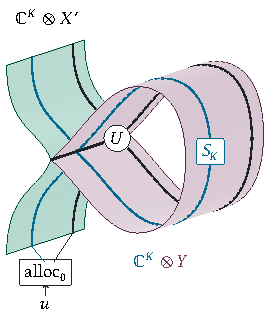
\includegraphics{figures/76-finite-counter-sheet.pdf}
\end{minipage}\hfill
\begin{minipage}{.61\linewidth}\raggedright
\setlength{\abovedisplayskip}{5pt}\setlength{\belowdisplayskip}{5pt}
The enlarged body and the count program are
\[
\begin{aligned}
 \beta_K&=d_K^{-1}\,;\,(I_{[K]}\otimes\beta)\,;\,d'_K\\
        &\quad;\,(I_{[K]\otimes b}\oplus(S_K\otimes I_c)),\\
 \mathsf{count}_K\,\beta
     &=\mathsf{alloc}_0\,;\,\mathsf{arr}
(\mathsf{trace}_{[K]\otimes c}\,\beta_K).
\end{aligned}
\]
Their matrices satisfy
\[
W_K=\sem{\beta_K}=\begin{pmatrix} I_K\otimes A&I_K\otimes B\\
S_K\otimes C&S_K\otimes D
 \end{pmatrix}.
\]
\begin{equation}\label{eq:count}
 \begin{aligned}
R_Ku&=(\Tr^{\C^K\otimes Y}W_K)(\ket0\otimes u)\\
     &=\sum_{k\ge0}\ket{k\bmod K}\otimes x_ku.
 \end{aligned}
\end{equation}
\end{minipage}
\caption{The count construction. Counter and payload are distinct
tensor wires on both sheets, shown in depth in
Figure~\ref{fig:28b-sheets-unrolled}(a). Only the returning counter
passes through $S_K$.}\label{fig:76-finite-counter-sheet}
\Description{The finite count program, its unitary matrix and first
call are placed beside its two-factor sheet diagram. Its coherent
closure returns the joint counter-and-data state.}
\end{figure}\par
\FloatBarrier
The first call of $W_K$ on $(\ket0\otimes u,0)$ emits
$\ket0\otimes Au$ and returns $\ket{1\bmod K}\otimes Cu$.
Here $\ket0$ is a prepared counter, while the bare $0$ is absent
amplitude. Closing $\C^K\otimes Y$ adds the exits, with the counter
advanced once on each return. Figure~\ref{fig:28b-sheets-unrolled}
follows three calls with $K>3$. The blue counter and black payload
travel together on each sheet. The right panel closes the original
body and adds its exits without count labels.
\par\begin{figure}[!htbp]\centering
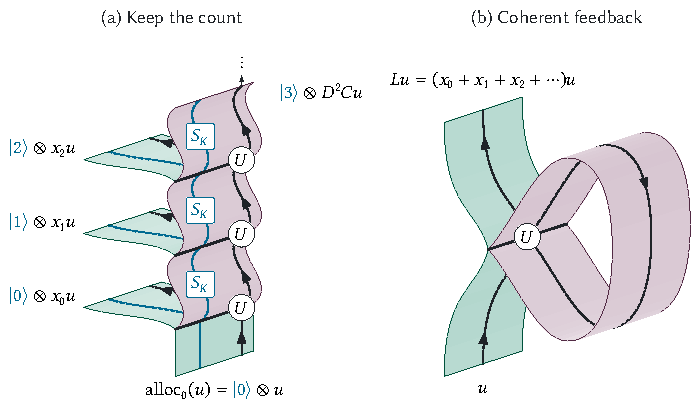
\includegraphics{figures/28b-sheets-unrolled.pdf}
\caption{After three calls of a $K>3$ clock, $\ket3\otimes D^2Cu$
continues past the arrow and dots. The right panel closes the
original body.}\label{fig:28b-sheets-unrolled}
\Description{A three-call clock unrolling has separate counter and
payload wires with explicit increments. The original closed loop has
one coherent output.}
\end{figure}\par

To hide the counter, first use the symmetry iso
$\sigma_{[K],b}:[K]\otimes b\leftrightarrow b\otimes[K]$. Hiding then
gives
$\mathsf{hide}(\mathsf{count}_K\beta;\mathsf{arr}\,\sigma_{[K],b})$.
Native \code{count} returns data first, so \code{discard} hides its
counter directly. Counts congruent modulo $K$ share a label, so their
amplitudes interfere before the clock is discarded. Hiding this
finite clock therefore need not give the measured loop.

Allocation is an isometry and the enlarged coherent loop is unitary,
so their composite $R_K$ is an isometry. Evaluation returns the joint
state without sampling a halting round.

An exact count uses $H_{\rm rec}=\ell^2(\N)$ and $Ru=\sum_k\ket
k\otimes x_ku$, with $\|Ru\|^2=\sum_k\|x_ku\|^2=\|u\|^2$. It is the
semantic limit of finite clocks. For the scalar rotation,
$R\ket*=\xi_{\rm rot}\otimes\ket*$ with unit count state $\xi_{\rm
rot}=t\ket0-s^2\sum_{k\ge1}t^{k-1}\ket k$. For \code{withReference},
the bypass instead has record $\ket0$:
$R\ket0=\ket0\otimes\ket0$, while
$R\ket1=\xi_{\rm rot}\otimes\ket1$. These different records of
the two arms make $R\ket+$ entangled.




For \code{guardRound} at $K=2$, the even-count amplitudes sum to
$t-s^2t/(1-t^2)=0$, and the odd-count amplitudes sum to
$-s^2/(1-t^2)=-1$. Its parity clock is therefore $-\ket1$.
The bypass retains label $\ket0$. The parity clock therefore
distinguishes the two arms. The joint output on $\ket+$ is
$(\ket0\ket0-\ket1\ket1)/\sqrt2$, so tracing out the clock leaves
$I/2$.

Including each finite counter in $H_{\rm rec}$, these outputs
converge in operator norm to the exact record $R$
(Appendix~\ref{app:readings}). A time-dependent model can keep the
same distinctions by making outputs from different calls arrive at
different times~\cite[\S~3.4]{AndresMartinez22Thesis}. Synchronizing
execution has a different purpose. The quantum control machine
synchronizes final control states~\cite{YuanVillanyiCarbin24QCM}, and
register-machine compilation obtains wait counts within a chosen time
bound~\cite[\S~5]{ZhangYing25QRM}. These address common-clock
halting~\cite{LindenPopescu98Halting} without requiring the program
to return a count register.

\subsection{Measure the returning tag}
To measure the guard without measuring the payload, allocate a fresh
bit at $0$ and flip it only on a \kw{back} tag. Hiding this copied
bit removes the cross terms between exit and return, while preserving
coherence within either payload. This works for unequal payloads, as
in \code{withReference}. The tag-copying isometry is
\[
T:b+c\rightarrowtail(b+c)\otimes\kw{Qubit},\qquad
 \mathsf{exit}\,x\mapsto\langle\mathsf{exit}\,x,0\rangle,
 \quad\mathsf{back}\,y\mapsto\langle\mathsf{back}\,y,1\rangle.
\]
The full reversible clauses are in Appendix~\ref{app:rules}. One call
is $\mathsf{hide}(\mathsf{arr}\,\beta;T)$, which keeps the payload
and removes only coherence between the two tags.

For a density input $\rho$ of trace one, the first call emits
$A\rho A^\dagger$ and returns $\sigma_1=C\rho C^\dagger$.
Subsequent calls emit $B\sigma_nB^\dagger$ and return
$\sigma_{n+1}=D\sigma_nD^\dagger$. The blocks are not normalized
after each call: $\tr\sigma_n$ is precisely the probability of still
being inside after $n$ calls. The emitted block on call
$k+1$ is $x_k\rho x_k^\dagger$. Adding these emitted blocks gives
the measured loop $\meas=\sem{\mathsf{while}_c\,\beta}$:
\begin{equation}\label{eq:meas}
 \meas(\rho)=\sum_{k\ge0}x_k\rho x_k^\dagger
=\tr_{H_{\rm rec}}(R\rho R^\dagger).
\end{equation}
The residual probability tends to zero by Theorem~\ref{thm:total}.
Thus a measured run halts after finitely many calls with probability
one, although there need not be a finite bound on its possible
halting rounds. Its output is a density operator on $\sem b$, with no
port tag or retained count. This differs from coherent evaluation,
which solves for a completed map without sampling a halting round.

For \code{withReference} on $\rho=\ket+\bra+$, the immediate exit is
the only one containing both paths. Its density matrix and the sum of
all later contributions are
\[
 \underbrace{\frac12\begin{pmatrix}1&t\\t&t^2\end{pmatrix}}_{\text
{immediate
 exit}}
+\underbrace{\frac{s^4}{2(1-t^2)}
       \begin{pmatrix}0&0\\0&1\end{pmatrix}}_{\text{later exits}}
=\frac12\begin{pmatrix}1&t\\t&1\end{pmatrix}.
\]
Here $s^4/(1-t^2)=s^2$, so the lower diagonal entry is
$(t^2+s^2)/2=1/2$. A final Hadamard followed by reading $1$ tests the
projection onto
$\ket-$. Its measured probability is $(1-t)/2=1/5$, whereas
the coherent output $\ket-$ gives probability one. Both predictions
therefore follow from the same three clauses.

Discarding the exact record gives the same mixture
in~\eqref{eq:meas}: tracing out $\ket k\bra j$ removes $k\ne j$ and
keeps $x_k\rho x_k^\dagger$ at $k=j$.

For general payloads, let
$(\rho,\sigma)$ be positive blocks on $X,Y$ with total trace at
most one. Applying $U$ to their block-diagonal matrix and retaining
the two diagonal output blocks gives the branching map
\[
 \Phi_U(\rho,\sigma)=
(A\rho A^\dagger+B\sigma B^\dagger,\quad C\rho C^\dagger+D\sigma
D^\dagger).
\]
Its two outputs are a classical alternative: their traces are the
weights on the exit and return branches. When $a=b=c$,
$\mathsf{factor}:a+a\leftrightarrow a\otimes\kw{Qubit}$ exposes the
tag. Its inverse $\mathsf{dist}$ restores the sum, so the left box in
Figure~\ref{fig:77-measured-sheet} is
$\widehat U=\sem{\mathsf{dist};\beta;\mathsf{factor}}$.
\sheetpic{77-measured-sheet}{At left (for $X=X'=Y$), the copied tag
is hidden inside each call, before the outgoing sheets separate. At
right, closing the returning classical block of $\Phi_U$ gives the
measured loop for general payloads.}{The copied tag is hidden inside
every call, before the outgoing sheets separate.}

Closing the return uses the established trace of completely positive
trace-nonincreasing maps on finite $C^*$-algebras, with their
classical sum~\cite[Prop.~3.2.17]{AndresMartinez22Thesis}:
\[
 \sem{\mathsf{while}_c\,\beta}
=\Tr^{\operatorname{End}(Y)}_{\rm cl}(\Phi_U)=\meas.
\]
Unrolling this trace gives the emitted blocks in~\eqref{eq:meas}.

Our body-first convention is obtained by applying $U$ once before the
published test-first loop~\cite[\S~3]{YingFeng10QuantumLoop}.
Appendix~\ref{app:readings} gives the correspondence.

Orthogonal exits in retained data can still have nonzero cross outer
products. An ignored count removes those terms; the two-exit cycle in
Appendix~\ref{app:programs} illustrates the distinction.

Allocation alone preserves coherent
feedback~\cite[Cor.~3.3.16]{AndresMartinez22Thesis}. Recording
changes the body by adding a counter and successor. Measurement
instead closes a classical alternative of operator blocks.

\par\noindent\begin{minipage}{\linewidth}
\begin{definition}[The three loop
readings]\label[definition]{def:three-loops}
Let $\beta:a+c\leftrightarrow b+c$ be finite, with exits $x_k$ and
$K\ge1$. The right column specializes to \code{withReference} on
$u=\ket+$ or $\rho=\ket+\bra+$, with $K=2$ and $t=3/5$.
\par\smallskip\centering
{\small\setlength{\tabcolsep}{4pt}\renewcommand{\arraystretch}{1.15}
\begin{tabular}{@{}lll@{}}
\textcolor{flipback}{$\mathsf{trace}_c\,\beta:a\leftrightarrow b$}
 & $\textcolor{flipback}{L}u=\sum_{k\ge0}x_ku$ & $\ket-$\\[5pt]
\textcolor{equalcount}{$\mathsf{count}_K\,\beta:a\rightarrowtail
[K]\otimes
b$}
 & $\textcolor{equalcount}{R_K}u=\sum_{k\ge0}\ket{k\bmod K}\otimes
 x_ku$
 &
 $\dfrac{\textcolor{equalcount}{\ket0}\ket0-\textcolor
{equalcount}{\ket1}\ket1}{\sqrt2}$\\[5pt]
\textcolor{accentwarm}{$\mathsf{while}_c\,\beta:a\rightsquigarrow b$}
 & $\textcolor{accentwarm}{\meas}(\rho)=\sum_{k\ge0}x_k\rho
 x_k^\dagger$
 & $\dfrac12\begin{pmatrix}1&t\\t&1\end{pmatrix}$
\end{tabular}}
\end{definition}
\end{minipage}\par


\FloatBarrier
\section{When can a caller forget the
difference?}\label{sec:agreement}
The Hadamard test distinguished the measured and coherent loops using
one output bit. We now ask when their channels are equal on
\emph{every} input, including data entangled with a caller's
reference. We call this \emph{free erasure} of the count. The
unitary-channel criterion is the rank-one case of uniqueness of
finite Kraus representations~\cite[Cor.~2.23]{Watrous18TQI}. Here its
Kraus operators are the body's successive exits. Their shared finite
return space makes the criterion a finite test on clauses. The scalar
rotation gives a first case of agreement: its count state is fixed,
so ignoring it cannot change the data. The following criterion
determines when the same is true for a general external interface.
\Needspace{9\baselineskip}
\begin{theorem}[Agreement on the data]\label{thm:axis}
Let $\beta:a+c\leftrightarrow b+c$ be a finite iso with nonempty
external type. Put $m=|\mathcal B(c)|$. The following conditions are
equivalent.
\begin{enumerate}
\item $\meas=\chan L$ as channels on the external data, where $\chan
L(\rho)=L\rho L^\dagger$.
\item There is a single unit vector $\xi\in\ell^2(\N)$ such that $R
u=\xi\otimes Lu$ for every $u$.
\item The $m+1$ operators $x_0,\ldots,x_m$ span a one-dimensional
subspace in the space of maps from $X$ to $X'$.
\end{enumerate}
In this case $x_k=b_kL$ for every $k$, with $\sum_k |b_k|^2=1$ and
$\sum_k b_k=1$.
\end{theorem}
For the scalar rotation, $Ru=\xi_{\rm rot}\otimes u =(-\xi_{\rm
rot})\otimes Lu$ since $Lu=-u$, so the fixed state in condition~(2)
is $-\xi_{\rm rot}$. For \code{withReference}, the return space still
has dimension $m=1$, but the first two exits are
\[
x_0=\operatorname{diag}(1,3/5),\qquad
x_1=\operatorname{diag}(0,-16/25).
\]
They cannot be multiples of one another, since the first is identity
on the bypass and the second is zero there. Thus the first two exits
already certify the difference observed by the Hadamard test in
Section~\ref{sec:effects}. Agreement also permits a loop to change
its data. Applying
$\mathsf X$ only on exit makes every exit a scalar multiple of
$\mathsf X$ and their sum $-\mathsf X$, so this variant passes.
Appendix~\ref{app:programs} gives its clauses and a two-section
cascade that also passes on non-scalar data.

Agreement concerns the specified interface. A channel identifies $I$
and $-I$, whereas a coherent bypass distinguishes $I\oplus I$ from
$I\oplus(-I)$. Such a bypass therefore has to be formed before
channelization, which preserves neither that coherent sum nor its
trace for arbitrary bodies~\cite[\S~3.3.3]{AndresMartinez22Thesis}.

The rank-one Kraus criterion gives $x_k=b_kL$, so $Ru=\xi\otimes Lu$
and tracing out the fixed count preserves $L\rho L^\dagger$.
Cayley--Hamilton then puts every later exit in the span of the first
$m+1$; at $m=0$, only $x_0=L$ remains. Exact coefficients with
decidable equality give the finite test, using any nonzero exit as
reference. Appendix~\ref{app:axis} proves the equivalences.

Figure~\ref{fig:trace-comparison} puts the two constructions beside
one another. Write $\operatorname{End}(X)$ for the matrix algebra on
$X$. The lower path uses the classical sum
$\operatorname{End}(X)\oplus\operatorname{End}(Y)$, whose inputs
are pairs of positive blocks. It differs from the coherent Hilbert
sum $X\oplus Y$ used on the upper path. The theorem says exactly when
closing these different kinds of return gives the same channel on the
external data.
\begin{figure}[!htbp]\centering
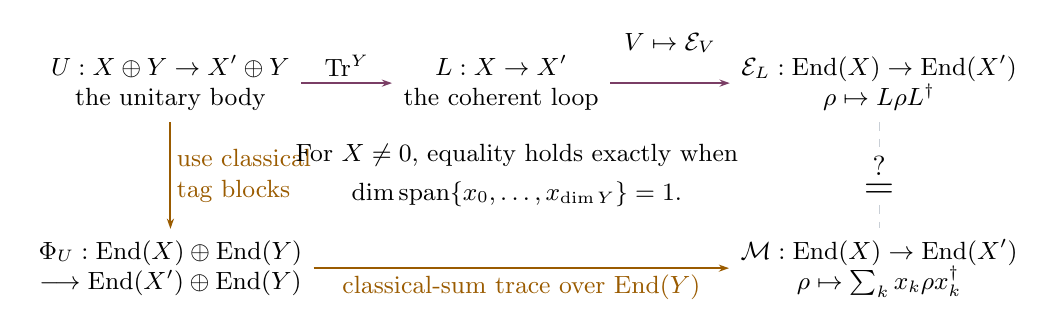
\begin{tikzpicture}[kme circuit,>={Stealth[length=1.3mm,width=.9mm]},
entry/.style={align=center,inner sep=4pt},
coh/.style={draw=flipback,line width=.7pt,->},
obs/.style={draw=accentwarm,line width=.7pt,->}]
 \node[entry] (u) at (0,2.35)
   {$U:X\oplus Y\to X'\oplus Y$\\the unitary body};
 \node[entry] (l) at (4.20,2.35)
   {$L:X\to X'$\\the coherent loop};
 \node[entry] (e) at (9.00,2.35)
   {$\chan L:\operatorname{End}(X)\to\operatorname{End}(X')$\\
    $\rho\mapsto L\rho L^\dagger$};
 \node[entry] (p) at (0,0)
   {$\Phi_U:\operatorname{End}(X)\oplus\operatorname{End}(Y)$\\
    $\longrightarrow\operatorname{End}(X')\oplus\operatorname
{End}(Y)$};
 \node[entry] (m) at (9.00,0)
   {$\meas:\operatorname{End}(X)\to\operatorname{End}(X')$\\
    $\rho\mapsto\sum_k x_k\rho x_k^\dagger$};
 \draw[coh] (u.east) -- node[above] {$\Tr^Y$} (l.west);
 \draw[coh] (l.east) -- node[above=3mm] {$V\mapsto\chan V$} (e.west);
 \draw[obs] (u.south) -- node[right,align=left,text=accentwarm]
   {use classical\\tag blocks} (p.north);
 \draw[obs] (p.east) -- node[below,text=accentwarm]
   {classical-sum trace over $\operatorname{End}(Y)$} (m.west);
 \draw[hairline,dashed] (e.south) -- (m.north);
 \node[fill=white,font=\Large] at (9.00,1.18) {$\stackrel{?}{=}$};
 \node[align=center] at (4.40,1.18)
   {For $X\ne0$, equality holds exactly when\\[3pt]
    $\dim\operatorname{span}\{x_0,\ldots,x_{\dim Y}\}=1$.};
\end{tikzpicture}
\caption{Two constructions from one body. The upper path closes
amplitudes before taking a data channel. The lower path uses
classical tag alternatives and then closes their return.
Theorem~\ref{thm:axis} decides whether the two resulting channels
coincide.}\label{fig:trace-comparison}
\Description{The coherent and classical trace paths end in two
separately displayed channels, compared by the finite exit-span
criterion. All maps have explicit domains and codomains.}
\end{figure}
\FloatBarrier

\paragraph{A program transformation.}
The Hadamard caller compares the loops as channels, using the
syntactic embedding $E(\omega)=\mathsf{arr}(\mathsf{arr}\,\omega)$,
which denotes $\chan{\sem\omega}$. Let
$\mathsf{prep}_+:1\rightsquigarrow\kw{Qubit}$ allocate $0$, remove
the unit factor and apply $H$, and let
$\mathsf{read}_Z:\kw{Qubit}\rightsquigarrow\kw{Qubit}$ be the
derived basis measurement, whose output records the classical
outcome. The context
\[
 \mathcal C[-]=\mathsf{prep}_+\,;\,[-]\,;\,E(H)\,;\,\mathsf{read}_Z
\]
has hole type $\kw{Qubit}\rightsquigarrow\kw{Qubit}$ and result type
$1\rightsquigarrow\kw{Qubit}$. Plugging in
$E(\kw{trace}\ \code{withReference})$ gives outcome $1$ with
probability one, while $\kw{while}\ \code{withReference}$ gives it
with probability $1/5$.

The permitted observers are channel contexts with one hole of type
$a\rightsquigarrow b$. For fixed closed channels $h,h_j$, their
grammar is
\[
\begin{aligned}
 \mathcal C&::=[-]\mid h;\mathcal C\mid\mathcal C;h
     \mid h\otimes\mathcal C\mid\mathcal C\otimes h\\
 &\quad\mid\mathsf{case}\bigl(\Psi_i;\mathcal C,
(\Psi_j;h_j)_{j\ne i}\bigr).
\end{aligned}
\]
The last constructor uses an instrument with a finite outcome set
$J$ and a chosen branch $i\in J$. Its completely positive maps
$\Psi_j:\operatorname{End}(\sem c)\to
\operatorname{End}(\sem{c_j})$ have output traces summing to one
on a density input. The trace of $\Psi_j(\rho)$ is the probability of
outcome $j$. Branch $i$ has payload type $c_i$, which the selected
context accepts; the other continuations accept their respective
$c_j$, and all branches return the same final type. The judgment
$a\rightsquigarrow b\vdash\mathcal C:c\rightsquigarrow d$ means
that plugging a program of the hole type gives a channel
$c\rightsquigarrow d$. Sequence matches intermediate types, while
tensor pairs the two inputs and the two outputs. The full rules are
in Appendix~\ref{app:axis}. Branching uses classical outcomes, so
these contexts supply no coherent control or coherent trace of the
channel hole.

More generally, on density input $\rho$ an output test $0\le P\le I$
has probability
$\tr(P\,\sem{\mathcal C[h]}(\rho))$. Two channel programs are
\emph{contextually equivalent} when these probabilities agree for
every well-typed context, input and test. Equality of channels
preserves them by induction on the grammar, including an entangled
reference in a tensor factor. Conversely, unequal channels have a
distinguishing input and output test already in the empty context.
\Needspace{5\baselineskip}
\begin{corollary}[Replacement]\label{cor:replace}
Dropping the exact record always gives \kw{while}. On nonempty
external data, an embedded \kw{trace} may replace \kw{while} in all
channel contexts exactly when the test of Theorem~\ref{thm:axis}
passes. Then dropping any finite clock gives the same channel. On
empty external data all these data channels coincide.
\end{corollary}
The exact record lies outside the finite grammar.
Appendix~\ref{app:axis} covers semantic continuations that carry it
without inspection and drop it on return.

Reading a fixed count still adds an observable output. Even when
$K=\dim Y$, a single clock can miss a failure of agreement.
On an external qubit, a permutation can have only $x_0=\ket0\bra0$
and
$x_K=\ket1\bra1$ as nonzero exits. Both receive clock label $0$,
so discarding that clock preserves $\ket+$, whereas measuring each
call gives $I/2$. Appendix~\ref{app:axis} gives the permutation.

\section{A count without a counter}\label{sec:phase}
The agreement test concerns channels on returned data. We now keep
the coherent iso before embedding it as a channel, so we can put it
beside the reference used in Section~\ref{sec:trace}. Changing the
phase on its return wire will reveal how its response depends on the
rounds.

A completed gate alone does not determine a count distribution: an
immediate phase $-1$ and \code{guardRound} both give $-1$, but only
\code{guardRound} has delayed exits. We distinguish them by inserting
a phase $z=e^{i\varphi}$ on the return port and varying it. The new
completed gate $\Theta(z)$ leaves an immediate exit unchanged and
multiplies exit $k$ by $z^k$, one factor for each return. This
\emph{transfer function} therefore generates the original exits.
Summing the marked exits will use an inverse on the returning space,
so we first separate the vectors that never emit. Define
\[
Y_0=\{y\in Y\mid BD^jy=0\text{ for every }j\ge0\},\qquad
Y_1=Y_0^\perp.
\]
By definition, $D(Y_0)\subseteq Y_0$ and $B|_{Y_0}=0$. Unitarity
gives $\|Dy\|^2+\|By\|^2=\|y\|^2$, so $D$ preserves norm on $Y_0$. In
finite dimension this restriction is onto. Unitarity then maps the
orthogonal complements of these internal components onto one another,
giving $C(X)\subseteq Y_1$ and
$D(Y_1)\subseteq Y_1$.
Put $B_1=B|_{Y_1}$ and $D_1=D|_{Y_1}$, regarding $C$ as
$X\to Y_1$. The geometric decay from Section~\ref{sec:trace} makes
$I-zD_1$ invertible for
$|z|\le1$, even when $I-zD$ on all of $Y$ is singular.
\par\begin{figure}[!htbp]\centering
\begin{minipage}{.39\linewidth}\centering
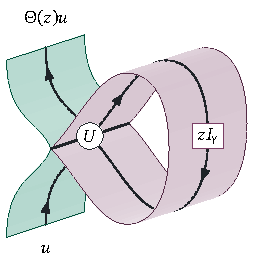
\includegraphics{figures/75-phased-sheet.pdf}
\end{minipage}\hfill
\begin{minipage}{.58\linewidth}\centering
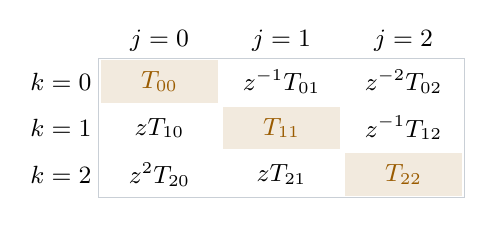
\begin{tikzpicture}[x=1.55cm,y=.59cm,every node/.style={inner
sep=1pt,font=\small}]
 \foreach \k in {0,1,2}{
  \node[anchor=east] at (-.53,-\k) {$k=\k$};
  \node at (\k,.87) {$j=\k$};
  \fill[accentwarm!13] (\k-.48,-\k-.46) rectangle (\k+.48,-\k+.46);
  \node[text=accentwarm] at (\k,-\k) {$T_{\k\k}$};
 }
 \node at (1,0) {$z^{-1}T_{01}$}; \node at (2,0) {$z^{-2}T_{02}$};
 \node at (0,-1) {$zT_{10}$}; \node at (2,-1) {$z^{-1}T_{12}$};
 \node at (0,-2) {$z^2T_{20}$}; \node at (1,-2) {$zT_{21}$};
 \draw[hairline] (-.5,.49) rectangle (2.5,-2.49);
\end{tikzpicture}\par
\(T_{kj}=x_k\rho x_j^\dagger\)
\[
 \begin{aligned}
 \Theta_{\rm rot}(z)&=\frac{t-z}{1-tz},\\
 \Theta_{\rm ref}(z)&=\operatorname{diag}(1,\Theta_{\rm rot}(z)).
 \end{aligned}
\]
\end{minipage}
\[
 \Theta(z)=\sum_{k\ge0}z^kx_k
=A+zB_1(I-zD_1)^{-1}C,\qquad L=\Theta(1).
\]
\caption{Each return adds a factor $z$ at left. In the channel at
right, exit pair $k,j$ carries $z^{k-j}T_{kj}$. Averaging over the
circle retains only the orange diagonal. The same cancellation
applies to later exits. The displayed families $\Theta_{\rm rot}$ and
$\Theta_{\rm ref}$ belong to \code{guardRound} and
\code{withReference}.}\label{fig:75-phased-sheet}\label
{fig:phase-grid}
\Description{The phase-marked return loop stands beside the matrix of
cross terms between exit counts. Its diagonal survives phase
averaging, giving the measured channel.}
\end{figure}\par

For the data channel, the term $x_k\rho x_j^\dagger$ carries phase
$e^{i(k-j)\varphi}$, as the right panel of
Figure~\ref{fig:phase-grid} shows. Averaging over the circle keeps
only $k=j$, so

\begin{equation}\label{eq:haar}
 \meas(\rho)=\frac1{2\pi}\int_0^{2\pi}
     \Theta(e^{i\varphi})\,\rho\,\Theta(e^{i\varphi})^\dagger
\,d\varphi
     .
\end{equation}
Thus the measured loop is a uniform mixture of coherent loops
differing only in their return phase. Geometric decay justifies these
Fourier manipulations.

Differentiation can recover a count because a single exit at count
$k$ has response $e^{ik\varphi}L$. Its derivative is $ik$ times that
response. Undoing the gate and multiplying by $-i$ gives $kI$. With
several exits there are also cross terms at a fixed phase. The
unitary transfer identity and the phase average from monitored
recurrence~\cite[Eq.~(4.10)]{BehrndtHassiSnoo09Colligations}~\cite[\S
~3,
Eq.~(8)]{Bourgain14Subspace} relate this coherent observable to the
measured mean.

\par\noindent\begin{minipage}{\linewidth}
\begin{theorem}[The measured mean and the phase
derivative]\label{thm:deriv}
Let $F_z=(I-zD_1)^{-1}C$ and $N=\sum_{k\ge0}k\,x_k^\dagger x_k$. For
$z=e^{i\varphi}$, the positive semidefinite relative phase derivative
and its average satisfy
\[
\begin{aligned}
Q(z)&=-i\Theta(z)^\dagger\frac{d}{d\varphi}\Theta(e^{i\varphi})
=F_z^\dagger F_z,\\
 \frac1{2\pi}\int_0^{2\pi}Q(e^{i\varphi})\,d\varphi
      &=N,\qquad \tr N=\dim Y_1.
\end{aligned}
\]
For unit $u\in X$, $\langle u,Nu\rangle$ is the measured mean number
of returns.
\end{theorem}
\end{minipage}\par
Appendix~\ref{app:deriv} differentiates $U$'s inner-product identity
and averages over phase. With $CC^\dagger=I_{Y_1}-D_1D_1^\dagger$
from unitarity, cyclicity and decay give the telescope
\[
 \tr N=\sum_{j\ge0}\tr\bigl(D_1^jCC^\dagger(D_1^\dagger)^j\bigr)
=\lim_{n\to\infty}\tr\bigl(I_{Y_1}-D_1^n(D_1^\dagger)^n\bigr) =\dim
Y_1.
\]

For a unit input $u$, prepare a reference bit in $\ket+$ to control
only the choice of return phase $z$ or $ze^{i\delta}$. The
$S^\dagger;H$ readout in Figure~\ref{fig:relative-hadamard} measures
the outputs' imaginary overlap, with inner products linear in the
second argument~\cite[p.~1, Eqs.~(1)--(3)]{Childs13Hadamard}.
Appendix~\ref{app:observing} gives its pure iso construction. Since
$Q(z)=F_z^\dagger F_z$, the first-order response gives the squared
norm of the returning amplitude before the phase gate. Several rounds
contribute to this wire, so its circulating weight can exceed one.
\begingroup\setlength{\intextsep}{6pt}
\begin{programfigure}\centering
\begin{minipage}{.63\linewidth}\centering
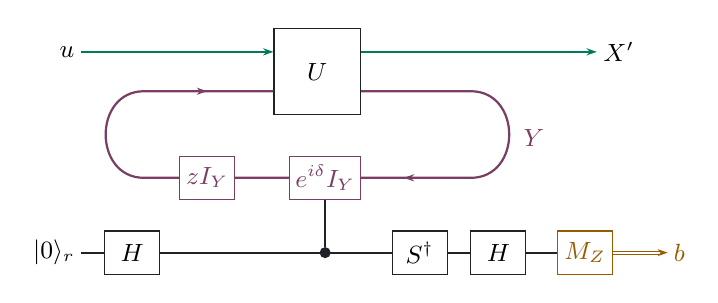
\begin{tikzpicture}[kme circuit,>={Stealth[length=1.3mm,width=.9mm]},
port/.style={draw=flipout,line width=.8pt},
ret/.style={draw=flipback,line width=.8pt}]
 \node[kme gate,minimum width=1.1cm,minimum height=1.10cm] (u) at
 (3.30,2.30) {$U$};
 \draw[port,->] (.30,2.55) node[left] {$u$} -- (u.west |- 0,2.55);
 \draw[port,->] (u.east |- 0,2.55) -- (6.85,2.55) node[right] {$X'$};
 \draw[ret] (u.east |- 0,2.05) -- (5.25,2.05)
.. controls (5.90,2.05) and (5.90,0.95) .. (5.25,0.95) -- (1.10,0.95)
.. controls (.45,0.95) and (.45,2.05) .. (1.10,2.05) -- (u.west |-
0,2.05);
 \draw[ret,->] (1.45,2.05) -- (1.90,2.05);
 \draw[ret,->] (4.80,0.95) -- (4.40,0.95);
 \node[kme gate,draw=flipback,text=flipback] at (1.90,0.95) {$zI_Y$};
 \node[kme gate,draw=flipback,text=flipback] (p) at (3.40,0.95)
 {$e^{i\delta}I_Y$};
 \node[text=flipback] at (6.05,1.45) {$Y$};
 \draw[kme wire] (.30,0) node[left] {$\ket0_r$} -- (6.35,0);
 \node[kme gate] at (.95,0) {$H$};
 \node[kme dot] (r) at (3.40,0) {};
 \draw[kme wire] (r) -- (p.south);
 \node[kme gate] at (4.60,0) {$S^\dagger$};
 \node[kme gate] at (5.60,0) {$H$};
 \node[kme gate,draw=accentwarm,text=accentwarm] (m) at (6.70,0)
 {$M_Z$};
 \draw[accentwarm,double,double distance=.65pt,->] (m.east) --
 (7.75,0) node[right] {$b$};
\end{tikzpicture}
\end{minipage}\hfill
\begin{minipage}{.34\linewidth}\centering
\(U:X\oplus Y\to X'\oplus Y\)\par\smallskip
\code{guardRound}, $u=1$
\[
\begin{gathered}
 \begin{array}{c|cc}
z&F_z&Q(z)\\ \hline
1&\textcolor{flipback}{s/(1-t)=2}&\textcolor{flipback}{4}\\[3pt]
-1&\textcolor{flipback}{s/(1+t)=1/2}&\textcolor{flipback}{1/4}
 \end{array}
\end{gathered}
\]
\(S^\dagger=\operatorname{diag}(1,-i)\)
\end{minipage}
\par\smallskip
\(\Pr(0)-\Pr(1)
=\operatorname{Im}\langle\Theta(z)u,\Theta(ze^{i\delta})u\rangle
=\delta\langle u,Q(z)u\rangle+O(\delta^2).\)
\caption{The reference chooses return phase $z$ or $ze^{i\delta}$ and
accompanies both summands unchanged through $U$. Its final
measurement reads the relative derivative. At right, $t=3/5$,
$s=4/5$, and $F_z$ is the scalar return amplitude before the phase
gate.}\label{fig:relative-hadamard}
\Description{A valid relative-phase Hadamard test is paired with the
exact scalar return amplitudes, their coherent squared weights, and
their circulating weights.}
\end{programfigure}
\endgroup

For \code{guardRound}, the measured mean is
$\textcolor{accentwarm}{\sum_{k\ge1}ks^4t^{2(k-1)}
=\sum_{j\ge0}s^2t^{2j}=s^2/(1-t^2)=1}$. The second sum adds survival
probabilities. The table beside the circuit instead squares the
summed return amplitudes, giving coherent weights $4$ and $1/4$.
Averaging $Q(z)$ over all phases recovers the measured mean.

The bypass in \code{withReference} makes no return, giving
$N_{\rm ref}=\operatorname{diag}(0,1)$. Its measured mean on
$\ket+$ is therefore $1/2$, the equal-weight average of bypass
count zero and scalar-loop mean one.

Putting return phase $z=e^{i\varphi}$ into the original Hadamard
caller gives these observable probabilities:
\[
\begin{array}{@{}c@{\qquad}c@{}}
 \Pr(b=1)=|1-\Theta_{\rm rot}(z)|^2/4
 &
\begin{array}{c|ccc}
 \varphi&0&\pi/2&\pi\\[2pt]
 \textcolor{flipback}{\Theta_{\rm rot}(e^{i\varphi})}
     &-1&(15-8i)/17&1\\[2pt]
 \textcolor{accentwarm}{\Pr(b=1)}&1&1/17&0
\end{array}
\end{array}
\]
Averaging this test over the phase circle gives the measured
probability $1/5$ by~\eqref{eq:haar}.


On a nonempty external type, agreement gives $\Theta(z)=f(z)L$ with
$|f(z)|=1$ on the circle, so every return phase gives the same data
channel. Conversely, if every phase channel equals $\chan L$, their
average is both $\chan L$ and $\meas$ by~\eqref{eq:haar}. Thus the
finite test also decides whether changing the return phase can affect
the data.

Appendix~\ref{sec:ring} realizes the scalar response with an ideal
lossless ring
coupler~\cite{Alsing17RingLoss,RaymerMcKinstrie13Cavity}.

\FloatBarrier
\section{The three readings in the \texorpdfstring{$\Pi$}{Pi}
family}\label{sec:family}

Figure~\ref{fig:pi-constructions} places the three readings in the
$\Pi$ family. A backwards wire is supplied by the
standard $\Int$ construction: its objects are pairs $(P^+,P^-)$, and
a map to $(Q^+,Q^-)$ is a unitary
$P^+\oplus Q^-\to Q^+\oplus P^-$. The fully faithful embedding
$N(X)=(X,0)$ preserves the sum
trace~\cite{JSV96,MalherbeScottSelinger12Partial}.
Appendix~\ref{app:diagrams} draws the typed components of this
bending.
\begingroup\setlength{\intextsep}{6pt}
\begin{programfigure}
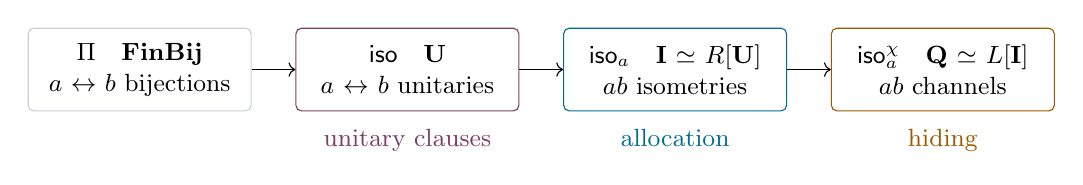
\begin{tikzpicture}[kme circuit,
stage/.style={draw=hairline,rounded corners=2pt,fill=white,
align=center,text width=2.55cm,minimum height=1.05cm,inner sep=4pt}]
 \node[stage] (p) at (0,0)
   {$\Pi\quad\mathbf{FinBij}$\\$a\leftrightarrow b$ bijections};
 \node[stage,draw=flipback] (u) at (3.40,0)
   {$\mathsf{iso}\quad\mathbf U$\\$a\leftrightarrow b$ unitaries};
 \node[stage,draw=equalcount] (i) at (6.80,0)
   {$\mathsf{iso}_a\quad\mathbf I\simeq R[\mathbf
   U]$\\$a\rightarrowtail b$ isometries};
 \node[stage,draw=accentwarm] (q) at (10.20,0)
   {$\mathsf{iso}_a^\chi\quad\mathbf Q\simeq L[\mathbf
   I]$\\$a\rightsquigarrow b$ channels};
 \draw[->] (p.east) -- (u.west);
 \draw[->] (u.east) -- (i.west);
 \draw[->] (i.east) -- (q.west);
 \node[below,text=flipback] at (3.40,-.68) {unitary clauses};
 \node[below,text=equalcount] at (6.80,-.68) {allocation};
 \node[below,text=accentwarm] at (10.20,-.68) {hiding};
\end{tikzpicture}\par\medskip
\begin{minipage}[t]{.32\linewidth}\centering
 \vspace{0pt}\textbf{Nested closure}\par\smallskip
 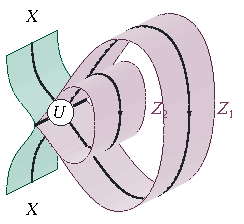
\includegraphics{figures/78-nested-sheets.pdf}\par
 \(\Tr^{Z_1}(\Tr^{Z_2}U)=\Tr^{Z_1\oplus Z_2}U\)
\end{minipage}\hfill
\begin{minipage}[t]{.32\linewidth}\centering
 \vspace{0pt}\textbf{A coherent bypass}\par\smallskip
 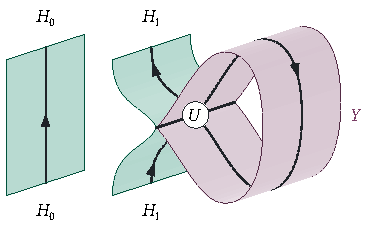
\includegraphics{figures/79-case-sheet.pdf}\par
 \(I\oplus\Tr^YU=\Tr^Y(I\oplus U)\)
\end{minipage}\hfill
\begin{minipage}[t]{.32\linewidth}\centering
 \vspace{0pt}\textbf{Sequence}\par\smallskip
 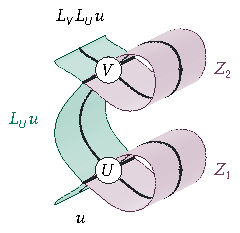
\includegraphics{figures/80-sequenced-sheets.pdf}\par
 \(\displaystyle\text{exit }k:\ \sum_{i+j=k}x_j^Vx_i^U\)
\end{minipage}
\caption{Finite source extensions and coherent trace laws for
endomorphisms~\cite
{HeunenKaarsgaard22Effects,JSV96,Bartha14QuantumTuringAutomata}.
Here $L=\sum_kx_k$ for each body, with returns kept in that body and
canonical
reassociations.}\label{fig:pi-constructions}\label{fig:sheet-laws}
\Description{Four language stages run left to right, adding unitary
clauses, allocation and hiding. Below them, three upward sheet
diagrams show nested feedback, a bypass and sequence at unchanged
label size.}
\end{programfigure}
\endgroup

\par\addvspace{\medskipamount}\noindent\textbf{AI Use.}
The author used ChatGPT Codex (GPT-6.1 Sol) to assist with paper
formatting, generating TikZ for figures, exploratory coding,
literature searches, and brainstorming of analytical approaches. The
author verified all results, revised the manuscript as needed, and
takes full responsibility for its content.

\par\addvspace{\smallskipamount}\noindent\textbf{Data-Availability
Statement.}
The paper and appendix contain rules, proofs and examples.

\clearpage

\begin{thebibliography}{23}


\ifx \showCODEN    \undefined \def \showCODEN     #1{\unskip}     \fi
\ifx \showISBNx    \undefined \def \showISBNx     #1{\unskip}     \fi
\ifx \showISBNxiii \undefined \def \showISBNxiii  #1{\unskip}     \fi
\ifx \showISSN     \undefined \def \showISSN      #1{\unskip}     \fi
\ifx \showLCCN     \undefined \def \showLCCN      #1{\unskip}     \fi
\ifx \shownote     \undefined \def \shownote      #1{#1}          \fi
\ifx \showarticletitle \undefined \def \showarticletitle #1{#1}   \fi
\ifx \showURL      \undefined \def \showURL       {\relax}        \fi
\providecommand\bibfield[2]{#2}
\providecommand\bibinfo[2]{#2}
\providecommand\natexlab[1]{#1}
\providecommand\showeprint[2][]{arXiv:#2}
\makeatletter
\@ifundefined{NAT@parse@date}{}{\let
\NAT@parse@date@orig\NAT@parse@date}
\@ifundefined{NAT@parse@date}{}{\def
\NAT@parse@date#1#2#3#4#5#6@@{\NAT@parse@date@orig#1#2#3#4#5#6@@\def
\NAT@tempyear{0000}\def\NAT@tempexlab{{?}}\ifx
\NAT@year\NAT@tempyear\ifx\NAT@exlab\NAT@tempexlab\def
\NAT@date{[n.\,d.]}\else\edef\NAT@date{[n.\,d.]\NAT@exlab}\fi\fi}}
\makeatother

\bibitem[Abramsky et~al\mbox{.}(2002)]{AbramskyHaghverdiScott02GoI}
\bibfield{author}{\bibinfo{person}{Samson Abramsky},
\bibinfo{person}{Esfandiar
Haghverdi}, {and} \bibinfo{person}{Philip Scott}.}
  \bibinfo{year}{2002}\natexlab{}.
\newblock \showarticletitle{Geometry of Interaction and linear
combinatory
algebras}.
\newblock \bibinfo{journal}{\emph{Mathematical Structures in Computer
Science}}
  \bibinfo{volume}{12}, \bibinfo{number}{5} (\bibinfo{year}{2002}),
  \bibinfo{pages}{625--665}.
\newblock
\href{https://doi.org/10.1017/S0960129502003730}{doi:\nolinkurl
{10.1017/S0960129502003730}}


\bibitem[Alsing et~al\mbox{.}(2017)]{Alsing17RingLoss}
\bibfield{author}{\bibinfo{person}{Paul~M. Alsing},
\bibinfo{person}{Edwin~E.
Hach, III}, \bibinfo{person}{Christopher~C. Tison}, {and}
  \bibinfo{person}{A.~Matthew Smith}.}
  \bibinfo{year}{2017}\natexlab{}.
\newblock \showarticletitle{Quantum-optical description of losses in
ring
resonators based on field-operator transformations}.
\newblock \bibinfo{journal}{\emph{Physical Review A}}
\bibinfo{volume}{95}
(\bibinfo{year}{2017}), \bibinfo{pages}{053828}.
\newblock
\showeprint[arxiv]{1608.01280}~[quant-ph]
\href{https://doi.org/10.1103/PhysRevA.95.053828}{doi:\nolinkurl
{10.1103/PhysRevA.95.053828}}


\bibitem[Andr{\'e}s-Mart{\'\i}nez(2022)]{AndresMartinez22Thesis}
\bibfield{author}{\bibinfo{person}{Pablo Andr{\'e}s-Mart{\'\i}nez}.}
  \bibinfo{year}{2022}\natexlab{}.
\newblock \emph{\bibinfo{title}{Unbounded loops in quantum programs:
categories
and weak while loops}}.
\newblock \bibinfo{thesistype}{Ph.\,D. Dissertation}.
  \bibinfo{school}{University of Edinburgh}.
\newblock
\showeprint[arxiv]{2212.05371}
\href{https://doi.org/10.48550/arXiv.2212.05371}{doi:\nolinkurl
{10.48550/arXiv.2212.05371}}


\bibitem[Bartha(2014)]{Bartha14QuantumTuringAutomata}
\bibfield{author}{\bibinfo{person}{Mikl{\'o}s Bartha}.}
  \bibinfo{year}{2014}\natexlab{}.
\newblock \showarticletitle{Quantum {T}uring automata}. In
  \bibinfo{booktitle}{\emph{Proceedings of DCM 2012}}
  \emph{(\bibinfo{series}{EPTCS}, Vol.~\bibinfo{volume}{143})}.
  \bibinfo{publisher}{Open Publishing Association},
  \bibinfo{address}{Waterloo,
NSW, Australia}, \bibinfo{pages}{17--31}.
\newblock
\showeprint[arxiv]{1404.0074}
\href{https://doi.org/10.4204/EPTCS.143.2}{doi:\nolinkurl
{10.4204/EPTCS.143.2}}


\bibitem[Behrndt et~al\mbox{.}(2009)]{BehrndtHassiSnoo09Colligations}
\bibfield{author}{\bibinfo{person}{Jussi Behrndt},
\bibinfo{person}{Seppo
Hassi}, {and} \bibinfo{person}{Henk de Snoo}.}
  \bibinfo{year}{2009}\natexlab{}.
\newblock \showarticletitle{Boundary Relations, Unitary Colligations,
and
Functional Models}.
\newblock \bibinfo{journal}{\emph{Complex Analysis and Operator
Theory}}
  \bibinfo{volume}{3}, \bibinfo{number}{1} (\bibinfo{year}{2009}),
  \bibinfo{pages}{57--98}.
\newblock
\href{https://doi.org/10.1007/s11785-008-0064-z}{doi:\nolinkurl
{10.1007/s11785-008-0064-z}}


\bibitem[Bourgain et~al\mbox{.}(2014)]{Bourgain14Subspace}
\bibfield{author}{\bibinfo{person}{J. Bourgain},
\bibinfo{person}{F.~A.
Gr{\"u}nbaum}, \bibinfo{person}{L. Vel{\'a}zquez}, {and}
\bibinfo{person}{J. Wilkening}.} \bibinfo{year}{2014}\natexlab{}.
\newblock \showarticletitle{Quantum Recurrence of a Subspace and
Operator-Valued {Schur} Functions}.
\newblock \bibinfo{journal}{\emph{Communications in Mathematical
Physics}}
  \bibinfo{volume}{329}, \bibinfo{number}{3} (\bibinfo{year}{2014}),
  \bibinfo{pages}{1031--1067}.
\newblock
\showeprint[arxiv]{1302.7286}
\href{https://doi.org/10.1007/s00220-014-1929-9}{doi:\nolinkurl
{10.1007/s00220-014-1929-9}}


\bibitem[Childs(2013)]{Childs13Hadamard}
\bibfield{author}{\bibinfo{person}{Andrew~M. Childs}.}
  \bibinfo{year}{2013}\natexlab{}.
\newblock \bibinfo{title}{Quantum Algorithms, Lecture 18:
Approximating the
Jones Polynomial}.
\newblock \bibinfo{howpublished}{University of Waterloo lecture
notes}.
\newblock
\urldef\tempurl\url
{https://www.cs.umd.edu/~amchilds/teaching/w13/l18.pdf}
\showURL{\tempurl}


\bibitem[Comfort et~al\mbox{.}(2020)]{ComfortDelpeuchHedges20Sheets}
\bibfield{author}{\bibinfo{person}{Cole Comfort},
\bibinfo{person}{Antonin
Delpeuch}, {and} \bibinfo{person}{Jules Hedges}.}
  \bibinfo{year}{2020}\natexlab{}.
\newblock \bibinfo{title}{Sheet diagrams for bimonoidal categories}.
\newblock
\showeprint[arxiv]{2010.13361}
\href{https://doi.org/10.48550/arXiv.2010.13361}{doi:\nolinkurl
{10.48550/arXiv.2010.13361}}


\bibitem[Fairbanks and Selinger(2025)]{FairbanksSelinger25Traces}
\bibfield{author}{\bibinfo{person}{Aaron~David Fairbanks} {and}
  \bibinfo{person}{Peter Selinger}.} \bibinfo{year}{2025}\natexlab{}.
\newblock \showarticletitle{On traces in categories of contractions}.
In
  \bibinfo{booktitle}{\emph{Proceedings of the 22nd International
  Conference on
Quantum Physics and Logic (QPL 2025)}}
\emph{(\bibinfo{series}{EPTCS}, Vol.~\bibinfo{volume}{426})},
\bibfield{editor}{\bibinfo{person}{Alejandro D{\'\i}az-Caro},
\bibinfo{person}{Ognyan Oreshkov}, {and}
  \bibinfo{person}{Ana~Bel{\'e}n Sainz}} (Eds.).
  \bibinfo{publisher}{Open
Publishing Association}, \bibinfo{address}{Waterloo, NSW, Australia},
  \bibinfo{pages}{79--99}.
\newblock
\showeprint[arxiv]{2502.14993}
\href{https://doi.org/10.4204/EPTCS.426.3}{doi:\nolinkurl
{10.4204/EPTCS.426.3}}


\bibitem[Gl{\"u}ck and Kaarsgaard(2018)]{GluckKaarsgaard18Flowchart}
\bibfield{author}{\bibinfo{person}{Robert Gl{\"u}ck} {and}
  \bibinfo{person}{Robin Kaarsgaard}.}
  \bibinfo{year}{2018}\natexlab{}.
\newblock \showarticletitle{A Categorical Foundation for Structured
Reversible
Flowchart Languages: Soundness and Adequacy}.
\newblock \bibinfo{journal}{\emph{Logical Methods in Computer
Science}}
  \bibinfo{volume}{14}, \bibinfo{number}{3}, Article
  \bibinfo{articleno}{16}
(\bibinfo{year}{2018}), \bibinfo{numpages}{38}~pages.
\newblock
\href{https://doi.org/10.23638/LMCS-14(3:16)2018}{doi:\nolinkurl
{10.23638/LMCS-14(3:16)2018}}
\newblock
\shownote{(arXiv:1710.03666)}.


\bibitem[Heunen and Kaarsgaard(2022)]{HeunenKaarsgaard22Effects}
\bibfield{author}{\bibinfo{person}{Chris Heunen} {and}
\bibinfo{person}{Robin
Kaarsgaard}.} \bibinfo{year}{2022}\natexlab{}.
\newblock \showarticletitle{Quantum information effects}.
\newblock \bibinfo{journal}{\emph{Proceedings of the ACM on
Programming
Languages}} \bibinfo{volume}{6}, \bibinfo{number}{POPL}
(\bibinfo{year}{2022}), \bibinfo{pages}{2:1--2:27}.
\newblock
\showeprint[arxiv]{2107.12144}
\href{https://doi.org/10.1145/3498663}{doi:\nolinkurl
{10.1145/3498663}}


\bibitem[James and Sabry(2013)]{JamesSabry13Interpreters}
\bibfield{author}{\bibinfo{person}{Roshan~P. James} {and}
\bibinfo{person}{Amr
Sabry}.} \bibinfo{year}{2013}\natexlab{}.
\newblock \showarticletitle{Isomorphic Interpreters from Logically
Reversible
Abstract Machines}. In \bibinfo{booktitle}{\emph{Reversible
Computation: 4th International Workshop, RC 2012, Revised Papers}}
  \emph{(\bibinfo{series}{Lecture Notes in Computer Science},
Vol.~\bibinfo{volume}{7581})}. \bibinfo{publisher}{Springer},
  \bibinfo{address}{Berlin, Heidelberg}, \bibinfo{pages}{57--71}.
\newblock
\href{https://doi.org/10.1007/978-3-642-36315-3_5}{doi:\nolinkurl
{10.1007/978-3-642-36315-3_5}}


\bibitem[Joyal et~al\mbox{.}(1996)]{JSV96}
\bibfield{author}{\bibinfo{person}{Andr{\'e} Joyal},
\bibinfo{person}{Ross
Street}, {and} \bibinfo{person}{Dominic Verity}.}
  \bibinfo{year}{1996}\natexlab{}.
\newblock \showarticletitle{Traced monoidal categories}.
\newblock \bibinfo{journal}{\emph{Mathematical Proceedings of the
Cambridge
Philosophical Society}} \bibinfo{volume}{119}, \bibinfo{number}{3}
(\bibinfo{year}{1996}), \bibinfo{pages}{447--468}.
\newblock
\href{https://doi.org/10.1017/S0305004100074338}{doi:\nolinkurl
{10.1017/S0305004100074338}}


\bibitem[Kaarsgaard and Rennela(2021)]{KaarsgaardRennela21JIRC}
\bibfield{author}{\bibinfo{person}{Robin Kaarsgaard} {and}
  \bibinfo{person}{Mathys Rennela}.} \bibinfo{year}{2021}\natexlab{}.
\newblock \showarticletitle{Join Inverse Rig Categories for
Reversible
Functional Programming, and Beyond}. In
\bibinfo{booktitle}{\emph{Proceedings of the 37th Conference on the
Mathematical Foundations of Programming Semantics (MFPS 2021)}}
\emph{(\bibinfo{series}{EPTCS}, Vol.~\bibinfo{volume}{351})}.
\bibinfo{publisher}{Open Publishing Association},
\bibinfo{address}{Waterloo, NSW, Australia},
  \bibinfo{pages}{152--167}.
\newblock
\href{https://doi.org/10.4204/EPTCS.351.10}{doi:\nolinkurl
{10.4204/EPTCS.351.10}}
\newblock
\shownote{(arXiv:2105.09929)}.


\bibitem[Lemonnier(2024)]{Lemonnier24}
\bibfield{author}{\bibinfo{person}{Louis Lemonnier}.}
  \bibinfo{year}{2024}\natexlab{}.
\newblock \emph{\bibinfo{title}{The Semantics of Effects: Centrality,
Quantum
Control and Reversible Recursion}}.
\newblock \bibinfo{thesistype}{Ph.\,D. Dissertation}.
  \bibinfo{school}{Universit\'e Paris-Saclay}.
\newblock
\showeprint[arxiv]{2406.07216}
\href{https://doi.org/10.48550/arXiv.2406.07216}{doi:\nolinkurl
{10.48550/arXiv.2406.07216}}


\bibitem[Linden and Popescu(1998)]{LindenPopescu98Halting}
\bibfield{author}{\bibinfo{person}{Noah Linden} {and}
\bibinfo{person}{Sandu
Popescu}.} \bibinfo{year}{1998}\natexlab{}.
\newblock \bibinfo{title}{The halting problem for quantum computers}.
\newblock
\showeprint[arxiv]{quant-ph/9806054}
\href{https://doi.org/10.48550/arXiv.quant-ph/9806054}{doi:\nolinkurl
{10.48550/arXiv.quant-ph/9806054}}


\bibitem[Malherbe
et~al\mbox{.}(2012)]{MalherbeScottSelinger12Partial}
\bibfield{author}{\bibinfo{person}{Octavio Malherbe},
\bibinfo{person}{Philip
Scott}, {and} \bibinfo{person}{Peter Selinger}.}
  \bibinfo{year}{2012}\natexlab{}.
\newblock \showarticletitle{Partially traced categories}.
\newblock \bibinfo{journal}{\emph{Journal of Pure and Applied
Algebra}}
  \bibinfo{volume}{216}, \bibinfo{number}{12} (\bibinfo{year}{2012}),
  \bibinfo{pages}{2563--2585}.
\newblock
\showeprint[arxiv]{1107.3608}
\href{https://doi.org/10.1016/j.jpaa.2012.03.026}{doi:\nolinkurl
{10.1016/j.jpaa.2012.03.026}}


\bibitem[Raymer and McKinstrie(2013)]{RaymerMcKinstrie13Cavity}
\bibfield{author}{\bibinfo{person}{M.~G. Raymer} {and}
\bibinfo{person}{C.~J.
McKinstrie}.} \bibinfo{year}{2013}\natexlab{}.
\newblock \showarticletitle{Quantum Input-Output Theory for Optical
Cavities
with Arbitrary Coupling Strength: Application to Two-Photon
Wave-Packet Shaping}.
\newblock \bibinfo{journal}{\emph{Physical Review A}}
\bibinfo{volume}{88}
(\bibinfo{year}{2013}), \bibinfo{pages}{043819}.
\newblock
\showeprint[arxiv]{1309.5915}~[quant-ph]
\href{https://doi.org/10.1103/PhysRevA.88.043819}{doi:\nolinkurl
{10.1103/PhysRevA.88.043819}}


\bibitem[Sabry et~al\mbox{.}(2018)]{SabryValironVizzotto18}
\bibfield{author}{\bibinfo{person}{Amr Sabry},
\bibinfo{person}{Beno{\^\i}t
Valiron}, {and} \bibinfo{person}{Juliana~Kaizer Vizzotto}.}
  \bibinfo{year}{2018}\natexlab{}.
\newblock \showarticletitle{From symmetric pattern-matching to
quantum
control}. In \bibinfo{booktitle}{\emph{FoSSaCS 2018}}.
  \bibinfo{publisher}{Springer}, \bibinfo{address}{Cham},
  \bibinfo{pages}{348--364}.
\newblock
\showeprint[arxiv]{1804.00952}
\href{https://doi.org/10.1007/978-3-319-89366-2_19}{doi:\nolinkurl
{10.1007/978-3-319-89366-2_19}}


\bibitem[Watrous(2018)]{Watrous18TQI}
\bibfield{author}{\bibinfo{person}{John Watrous}.}
  \bibinfo{year}{2018}\natexlab{}.
\newblock \bibinfo{booktitle}{\emph{The Theory of Quantum
Information}}.
\newblock \bibinfo{publisher}{Cambridge University Press},
  \bibinfo{address}{Cambridge, UK}.
\newblock
\href{https://doi.org/10.1017/9781316848142}{doi:\nolinkurl
{10.1017/9781316848142}}


\bibitem[Ying and Feng(2010)]{YingFeng10QuantumLoop}
\bibfield{author}{\bibinfo{person}{Mingsheng Ying} {and}
\bibinfo{person}{Yuan
Feng}.} \bibinfo{year}{2010}\natexlab{}.
\newblock \showarticletitle{Quantum loop programs}.
\newblock \bibinfo{journal}{\emph{Acta Informatica}}
\bibinfo{volume}{47},
  \bibinfo{number}{4} (\bibinfo{year}{2010}),
  \bibinfo{pages}{221--250}.
\newblock
\showeprint[arxiv]{quant-ph/0605218}
\href{https://doi.org/10.1007/s00236-010-0117-4}{doi:\nolinkurl
{10.1007/s00236-010-0117-4}}


\bibitem[Yuan et~al\mbox{.}(2024)]{YuanVillanyiCarbin24QCM}
\bibfield{author}{\bibinfo{person}{Charles Yuan},
\bibinfo{person}{Agnes
Villanyi}, {and} \bibinfo{person}{Michael Carbin}.}
  \bibinfo{year}{2024}\natexlab{}.
\newblock \showarticletitle{Quantum control machine: the limits of
control flow
in quantum programming}.
\newblock \bibinfo{journal}{\emph{Proc. ACM Program. Lang.}}
  \bibinfo{volume}{8}, \bibinfo{number}{OOPSLA1}
  (\bibinfo{year}{2024}),
  \bibinfo{pages}{1--28}.
\newblock
\showeprint[arxiv]{2304.15000}
\href{https://doi.org/10.1145/3649811}{doi:\nolinkurl
{10.1145/3649811}}


\bibitem[Zhang and Ying(2025)]{ZhangYing25QRM}
\bibfield{author}{\bibinfo{person}{Zhicheng Zhang} {and}
  \bibinfo{person}{Mingsheng Ying}.} \bibinfo{year}{2025}\natexlab{}.
\newblock \showarticletitle{Quantum register machine: efficient
implementation
of quantum recursive programs}.
\newblock \bibinfo{journal}{\emph{Proceedings of the ACM on
Programming
Languages}} \bibinfo{volume}{9}, \bibinfo{number}{PLDI}, Article
  \bibinfo{articleno}{180} (\bibinfo{year}{2025}),
  \bibinfo{numpages}{26}~pages.
\newblock
\showeprint[arxiv]{2408.10054}
\href{https://doi.org/10.1145/3729283}{doi:\nolinkurl
{10.1145/3729283}}


\end{thebibliography}

\appendix
\section{Typing and interpreting the clauses}\label{app:rules}
\subsection{Syntax}
\begin{figure}[!htbp]
\centering
\(\begin{aligned}
a,b &::= 0\mid 1\mid a+b\mid a\otimes b\\ v &::= *\mid
x\mid\mathrm{left}\ v\mid\mathrm{right}\ v\mid\langle v,v\rangle
       \mid\mathsf{exit}\ v\mid\mathsf{back}\ v\\
p,q &::= *\mid x\mid\langle p,q\rangle\\ e &::= v\mid
{\textstyle\sum_i}\alpha_i e_i
       \mid\mathsf{let}\ p=\omega\,q\ \mathsf{in}\ e\\
 \omega &::= f\mid\{v_i\leftrightarrow e_i\}_{i\in I}
    \mid\omega\,;\,\omega\mid\omega\oplus\omega\mid\omega\otimes
\omega
    \mid\omega^\dagger\mid\mathsf{trace}_{c}\,\omega\\
t &::= e\mid\omega\,t\\
 \mathit{decl} &::= f\mathbin{::}a\leftrightarrow b\ ;\ f=\omega
     \mid \mathsf{round}\ f:a+c=\{v_i\leftrightarrow e_i\}_{i\in I}
\end{aligned}\)
\caption{Finite iso definitions. A name $f$ refers to an earlier
closed definition. The coefficient $\alpha_i$ is a complex scalar. A
signature uses $::$, while the \kw{round} abbreviation uses $:$. The
subscript in $\mathsf{trace}_c$ identifies the return
type.}\label{fig:syntax}
\Description{The grammar separates types, patterns, expressions and
reversible definitions.}
\end{figure}\FloatBarrier
The surface patterns $\mathsf{exit}\,v$ and $\mathsf{back}\,v$
elaborate recursively to $\mathrm{left}\,v$ and $\mathrm{right}\,v$.
This rewrite preserves payloads and nesting, and is performed before
matching or typing by the core rules below. The remaining executable
abbreviations are those of Section~\ref{sec:iso}: \kw{Unit},
\code{unit}, \kw{Qubit} and its basis values, bracketed scalar
combinations, flow composition and \code{on} application. Listings
typeset the source token \code{<->} as $\leftrightarrow$ and pair
delimiters \code{<}, \code{>} as $\langle$, $\rangle$.

\subsection{Statics}
Admission, elaboration and evaluation are defined together by
induction over the ordered declarations and proper subprograms. In
particular, evaluating a local call to fill a table column uses a
proper subprogram or an already checked earlier definition. The
grammar in Figure~\ref{fig:syntax} describes definitions in an
ordered environment $\Sigma$. A binding $f=\omega:a\leftrightarrow b$
is introduced after checking $\omega$ against earlier bindings. Write
$\Sigma\ \mathsf{ok}$ when these declarations form a well-typed
environment. Types are the finite trees of Figure~\ref{fig:syntax}.
Both $0$ and $1$ are types, and $a+b$ and $a\otimes b$ are types
whenever $a$ and $b$ are. Names may be chosen fresh by renaming. The
rules for introducing them are
\[
 \frac{}{\varnothing\ \mathsf{ok}}\qquad
 \frac{\Sigma\ \mathsf{ok}\quad f\notin\operatorname{dom}(\Sigma)
       \quad\Sigma\vdash\omega:a\leftrightarrow b}
      {\Sigma,(f=\omega:a\leftrightarrow b)\ \mathsf{ok}}.
\] The declaration
\[
  \kw{round}\ f:a+c=\{v_i\leftrightarrow e_i\}_{i\in I}
\]
introduces the ordinary binding $f=\{v_i\leftrightarrow e_i\}_{i\in
I}:(a+c)\leftrightarrow(a+c)$ after the literal clauses have passed
the same check. The name denotes the open round. Closing it requires
an explicit operation. Writing $\Sigma\vdash d\Rightarrow\Sigma'$ for
declaration elaboration, its rule is
\[
 \frac{\Sigma\ \mathsf{ok}\quad
 f\notin\operatorname{dom}(\Sigma)\quad
       \Sigma\vdash\mathcal T:(a+c)\leftrightarrow(a+c)}
      {\Sigma\vdash\kw{round}\ f:a+c=\mathcal T
          \Rightarrow\Sigma,(f=\mathcal
          T:(a+c)\leftrightarrow(a+c))}.
\]
An ordinary iso signature still permits distinct external types. The
binding $f=\omega:a\leftrightarrow b$ represents the surface
declaration $f\mathbin{::}a\leftrightarrow b\ ;\ f=\omega$; listings
may separate these parts by a newline. Write $\Delta$ for a finite
set of distinct typed value variables. In $\Delta_1,\Delta_2$ the two
domains must be disjoint. Each judgment below uses this convention,
including inside a clause with an empty set of variables. The empty
table presents the unique map on $0$. Whenever we use a unit input or
a nonzero operator line we assume the corresponding external type is
inhabited.

\paragraph{Patterns and expressions.}
The finite basis is defined recursively:
\[
\begin{aligned}
 \mathcal B(0)&=\varnothing,& \mathcal B(1)&=\{*\},\\
 \mathcal B(a+b)&=\mathrm{left}\,\mathcal B(a)\ \sqcup\
 \mathrm{right}\,\mathcal B(b),
 &\mathcal B(a\otimes b)&=\mathcal B(a)\times\mathcal B(b).
\end{aligned}
\]
An environment for $\Delta$ assigns each variable a basis value of
its type. A variable matches any such value; a constructor matches
its own tag, and a pair matches its two components. Write
$\Delta\vdash v:a$ when a basis pattern is well typed. The rules are
\begin{mathpar}
 \isorule{}{\,\varnothing\vdash *:1}
 \and \isorule{}{x:a\vdash x:a}
 \and \isorule{\Delta\vdash v:a}{\Delta\vdash\mathrm{left}\ v:a+b}
 \and \isorule{\Delta\vdash v:b}{\Delta\vdash\mathrm{right}\ v:a+b}\\
 \isorule{\Delta_1\vdash v:a\\\Delta_2\vdash w:b}
       {\Delta_1,\Delta_2\vdash\langle v,w\rangle:a\otimes b}.
\end{mathpar}
For a context $\Delta$, let $\mathcal B(\Delta)$ be its basis
assignments and $\mathcal H(\Delta)=\mathbb C^{\mathcal B(\Delta)}$.
A product pattern $p$ with $\Delta\vdash p:b$ gives a bijection
$\gamma\mapsto p[\gamma]$ from $\mathcal B(\Delta)$ to $\mathcal
B(b)$. For unit it maps the unique empty assignment to $*$. For a
variable it is the identity. For a pair, disjoint contexts let us
combine the two component assignments uniquely. Induction on these
three rules proves the bijection, including empty bases. Matching $p$
is its inverse.

The unit, variable and pair rules also type the product patterns
$p,q$ in Figure~\ref{fig:syntax}. In the argument position $q$ these
rules assemble already bound values. In the result position $p$ they
bind fresh variables of the indicated types. A single variable in
either position may stand for a value of any type. For expressions we
write $\Sigma;\Delta\vdash e:a$ and use
\begin{mathpar}
 \isorule{\Delta\vdash v:a}{\Sigma;\Delta\vdash v:a}
 \and
 \isorule{\Sigma;\Delta\vdash e_i:a\ (i\in I)\\\alpha_i\in\C}
      {\Sigma;\Delta\vdash\sum_{i\in I}\alpha_i e_i:a}\\
 \isorule{\Delta_1\vdash q:a\\\Sigma\vdash\omega:a\leftrightarrow b\\
             \Delta_p\vdash p:b\\\Sigma;\Delta_2,\Delta_p\vdash e:d}
     {\Sigma;\Delta_1,\Delta_2\vdash
        \mathsf{let}\ p=\omega\,q\ \mathsf{in}\ e:d}.
\end{mathpar}
In the last rule the variables in $p$ are fresh and pairwise
distinct. A product pattern of type $b$ binds every basis output, by
the bijection above. The sum rule permits an empty index set in any
stated context $\Delta$; its denotation is the zero linear map from
$\mathcal H(\Delta)$. Such an expression cannot supply an entire
column of a nonempty unitary table. A finite first-order term is a
closed expression, or an application of a closed iso to a term of its
domain. Writing $\Sigma\vdash t:a$ for a closed term, its rules are
\[
 \frac{\Sigma;\varnothing\vdash e:a}{\Sigma\vdash e:a}
 \qquad
 \frac{\Sigma\vdash t:a\qquad\Sigma\vdash\omega:a\leftrightarrow b}
      {\Sigma\vdash\omega\,t:b}.
\]
This suffices for feeding a superposition of ground values to a
program.

For a matrix $M$ with input columns $s$ and output rows $t$, row $s$
of $M^\dagger$ is the conjugate of column $s$ of $M$. Consequently
its Gram matrix has entries
\[
(M^\dagger M)_{ss'}=
 \sum_{t\in\mathcal B(b)}\overline{M_{ts}}M_{ts'}.
\]
Each product pairs amplitudes in the same output row. At $s=s'$ it
contributes to the squared norm of one column; at $s\ne s'$ it
contributes to the inner product between two columns.

Let $M$ have one column for each $s\in\mathcal B(a)$, filled with the
coefficients of the expression in the uniquely matching clause under
its ground substitution. The following rule imposes a finite
extensional check. Its orthogonality premise concerns fully expanded
outputs, so it need not infer linear independence from surface
syntax.
\begin{mathpar}
\isorule{\Delta_i\vdash v_i:a\quad \Sigma;\Delta_i\vdash
e_i:b\quad(i\in I)\\
   \bigl(v_i[\mathcal B(\Delta_i)]\bigr)_{i\in I}\ \text{disjointly
   covers }\mathcal B(a)\\
|\mathcal B(a)|=|\mathcal B(b)|\quad M^\dagger M=I}
  {\Sigma\vdash\{v_i\leftrightarrow e_i\}_{i\in I}:a\leftrightarrow
  b}
\end{mathpar}
Here $v_i[\mathcal B(\Delta_i)]$ is the set of all ground instances
of pattern $v_i$. The coverage premise requires these sets to be
disjoint and their union to be $\mathcal B(a)$. An empty instance set
is permitted and contributes no column. This rule is exact over a
specified coefficient domain with exact equality and arithmetic, for
example rational complex numbers. With mathematical complex
parameters it is a well-formedness predicate; exact equality of
arbitrary descriptions of complex numbers is not assumed decidable.
The finite semantics does not make floating-point tolerance an
orthogonality proof.

\paragraph{Reversible combinators.}
For $M\in\C^{\mathcal B(b)\times\mathcal B(a)}$ the atom rule is
\[
 \frac{|\mathcal B(a)|=|\mathcal B(b)|\qquad M^\dagger M=I}
      {[M]:a\leftrightarrow b}.
\]
Omit the common $\Sigma$ in the following rules. A bound name has the
type at its declaration. For finite types we have the structural isos
of $\Pi$ as abbreviations for the corresponding permutation clauses,
including identity, symmetries and distributivity. The reversible
rules are
\begin{mathpar}
 \isorule{f:a\leftrightarrow b\in\Sigma}{f:a\leftrightarrow b}
 \and\isorule{u:a\leftrightarrow b\\v:b\leftrightarrow d}
                   {u\,;\,v:a\leftrightarrow d}
 \and\isorule{u:a\leftrightarrow b}{u^\dagger:b\leftrightarrow a}\\
 \isorule{u:a\leftrightarrow b\\v:d\leftrightarrow f}
            {u\oplus v:a+d\leftrightarrow b+f}
 \and\isorule{u:a\leftrightarrow b\\v:d\leftrightarrow f}
            {u\otimes v:a\otimes d\leftrightarrow b\otimes f}
 \and\isorule{\beta:a+c\leftrightarrow b+c}
            {\mathsf{trace}_c\,\beta:a\leftrightarrow b}.
\end{mathpar}

\subsection{Dynamics}
\paragraph{Evaluating an expression.}
Let $\gamma\in\mathcal B(\Delta)$ assign basis values to the
variables in a linear context $\Delta$, and write $\gamma\vdash
e\Downarrow\psi$ when evaluation returns the finite output vector
$\psi$. For a value pattern $v$, $v[\gamma]$ is its ground instance.
Values and sums evaluate by
\[
 \frac{}{\gamma\vdash v\Downarrow\ket{v[\gamma]}}
 \qquad
 \frac{\gamma\vdash e_i\Downarrow\psi_i\ (i\in I)}
      {\gamma\vdash\sum_i\alpha_i e_i\Downarrow\sum_i\alpha_i\psi_i}.
\]
For $\mathsf{let}\ p=\omega q\ \mathsf{in}\ e$, split the input
assignment as $\gamma_1\uplus\gamma_2$ according to the typing rule:
$q$ uses precisely $\gamma_1$, and $e$ retains $\gamma_2$. Write
$U\ket{q[\gamma_1]}=\sum_t a_t\ket t$, where $\omega\Downarrow U$.
Matching the product pattern $p$ with $t$ gives the fresh assignment
$\gamma_t$. The application rule is
\[
 \frac{\omega\Downarrow U\quad\gamma_2\uplus\gamma_t\vdash
 e\Downarrow\psi_t
          \quad(t\in\mathcal B(b))}
      {\gamma_1\uplus\gamma_2\vdash
        \mathsf{let}\ p=\omega q\ \mathsf{in}\ e
          \Downarrow\sum_t a_t\psi_t}.
\]
Here $b$ is the output type of $\omega$. Its admitted matrix supplies
the coefficients $a_t$, and total matching of $p$ supplies each
$\gamma_t$. The same binding is used independently in the
alternatives of a sum; it is split only where the linear typing rule
splits it. For closed terms, $t\Downarrow\psi$ uses the empty
variable assignment, with
\[
 \frac{\varnothing\vdash e\Downarrow\psi}{e\Downarrow\psi}
 \qquad
 \frac{\omega\Downarrow U\qquad t\Downarrow\psi}{\omega t\Downarrow
 U\psi}.
\]
The fixed iso environment is omitted from these evaluation judgments.
Named matrices are computed from earlier definitions; the reversible
combinators act by their matrix operations, and a trace uses
Proposition~\ref{prop:elim}. Thus expression evaluation is finite
even when its matrix contains feedback with infinitely many nonzero
exits. Induction on an expression's typing derivation shows that
evaluation gives its linear interpretation: the value rule
substitutes basis values, the sum rule is linearity, and the
application rule composes the admitted iso with the continuation's
linear map. These rules do not select a measurement outcome or
normalize individual amplitude components. More explicitly, the local
application's column at $(\gamma_1,\gamma_2)$ is
\[
E_{\mathsf{let}}(s;\gamma_1,\gamma_2) =\sum_{t\in\mathcal B(b)}
U_{t,q[\gamma_1]}\,E_e(s;\gamma_2,\gamma_t).
\]
Here $s\in\mathcal B(d)$ indexes the continuation output, and
$t\in\mathcal B(b)$ indexes the intermediate output of the local iso.
This is ordinary matrix multiplication: reassemble $q$'s variables,
apply $U$ while carrying $\gamma_2$, match its output to the fresh
product pattern, and apply the continuation matrix. The two pattern
maps are the bijections just proved. Thus the rule acts linearly on
arbitrary superpositions of assignments, including entangled ones. It
neither duplicates an assignment nor measures the local result.


\paragraph{Elaboration and matrix evaluation.}
The matrix programs have grammar
\[
 \kappa::=[M]\mid\kappa;\kappa\mid\kappa\oplus\kappa
       \mid\kappa\otimes\kappa\mid\kappa^\dagger
       \mid\mathsf{trace}_c\,\kappa.
\]

The combinators $\kappa$ of Section~\ref{sec:iso} have ground checked
tables as atoms. Write $\mathcal E_\Sigma(\omega)$ for elaboration.
If $f=\omega_f$ is a declaration in $\Sigma$, let $\Sigma_f$ be its
earlier prefix, the environment in which $\omega_f$ was checked. With
$M$ the evaluated columns of a table $\mathcal T$, the definition is
\[
\begin{aligned}
 \mathcal E_\Sigma(\mathcal T)&=[M],&
 \mathcal E_\Sigma(f)&=\mathcal E_{\Sigma_f}(\omega_f),\\
 \mathcal E_\Sigma(\omega;\nu)&=\mathcal E_\Sigma(\omega);\mathcal
 E_\Sigma(\nu),&
 \mathcal E_\Sigma(\omega\oplus\nu)&=\mathcal
 E_\Sigma(\omega)\oplus\mathcal E_\Sigma(\nu),\\
 \mathcal E_\Sigma(\omega\otimes\nu)&=\mathcal
 E_\Sigma(\omega)\otimes\mathcal E_\Sigma(\nu),&
 \mathcal E_\Sigma(\omega^\dagger)&=\mathcal
 E_\Sigma(\omega)^\dagger,\\
 \mathcal
 E_\Sigma(\mathsf{trace}_c\,\omega)&=\mathsf{trace}_c\,\mathcal
 E_\Sigma(\omega).
\end{aligned}
\]
These equations recurse into proper subprograms and, on lookup,
earlier definitions. Computing a table uses this same evaluation on
its local iso subprograms. This is a well-founded mutual definition
with expression evaluation. Each clause of the definition preserves
its source and target types. The declaration rule for \kw{round}
binds this open combinator and does not insert a trace.

If $\kappa\Downarrow M$ and $\lambda\Downarrow N$, the ordinary
matrix rules, used with their typed premises, are
\[
\begin{aligned}
 [M]&\Downarrow M,&(\kappa;\lambda)&\Downarrow NM,\\
(\kappa\oplus\lambda)&\Downarrow M\oplus N,&
(\kappa\otimes\lambda)&\Downarrow M\otimes N,&
 \kappa^\dagger&\Downarrow M^\dagger.
\end{aligned}
\]
The feedback rule completes them:
\[
 \frac{\kappa\Downarrow U\quad
U=\left(\begin{smallmatrix}A&B\\C&D\end{smallmatrix}\right)
       \quad F:X\to Y\quad (I_Y-D)F=C}
      {\mathsf{trace}_c\,\kappa\Downarrow A+BF}.
\]
The premise solves a finite linear system. It neither inverts a
possibly singular $I-D$ nor requires an execution to reach a last
exit. Theorem~\ref{thm:total} gives a solution and proves that every
solution gives the same output. Proposition~\ref{prop:elim} computes
that output by eliminating one return pattern at a time. Thus this
relational evaluation has a result independent of the chosen wire
solution, and exact elimination implements it. Write
$\Sigma\vdash\omega\Downarrow M$ when its elaboration evaluates to
$M$. Closed application then uses
\[
 \frac{\Sigma\vdash\omega\Downarrow M\qquad t\Downarrow\psi}
      {\omega t\Downarrow M\psi}.
\]
For a well-typed expression and a basis assignment, induction on its
syntax gives a unique output vector. In the local-binding case, the
argument and result patterns give inverse assembly/matching
bijections, and the finite coefficient sum is the matrix product
displayed above. Expanding each clause therefore preserves all its
columns. Induction through the combinators preserves evaluation and
the linear denotation; the trace case uses the feedback theorem.
Linearity then gives the same result on arbitrary superpositions,
including assignments entangled with a retained factor.

The executable listings use a finite clause frontend and a flow
frontend for the surrounding combinators. Their flow spellings are
$;$ for sequence, $+$ for direct sum and $*$ for tensor. Adjoint is
available mathematically by transposing and conjugating the ground
table. Unit and nested local patterns, the empty type and the empty
table belong to the mathematical grammar; the listings use variable
or flat-tuple local bindings and inhabited finite types. Native
numerical evaluation uses floating-point coefficients and may refuse
a coupled near-unit pivot; it is not the exact field-arithmetic
procedure of Proposition~\ref{prop:elim}.

\subsection{Denotation}
A checked table denotes the linear extension of its columns. Names,
sequence, dagger, direct sum and tensor denote lookup, composition in
execution order, adjoint, direct sum and tensor; trace denotes the
exit sum~\eqref{eq:exits}. The evaluation identities above give these
same maps, with the trace case supplied by Theorem~\ref{thm:total}.

Control of an endo-iso $u$ is $I\oplus u$ under the distributive iso
for $(1+1)\otimes a$. Thus controlling a global phase can change a
relative phase. The types above deliberately do not provide this
operation on an arbitrary channel.

\subsection{Effect extensions}
\paragraph{Syntax.}
Write $u$ for a reversible iso, $v$ for an isometry program and $h$
for a channel program. The two upper grammars are
\[
\begin{aligned}
v&::=\mathsf{arr}\,u\mid\mathsf{lift}\,u\mid v\,;\,v\mid v\oplus v
                         \mid v\otimes v\mid \mathsf{count}_K\,u,\\
h&::=\mathsf{arr}\,v\mid\mathsf{hide}\,v\mid h\,;\,h\mid h\otimes h
                         \mid\mathsf{while}_c\,u .
\end{aligned}
\]
\paragraph{Statics.}
The type of the intermediate result must match the type expected by
the next program. At the isometry layer this gives the following
rules for sequence, tensor and direct sum.
\begin{mathpar}
 \isorule{v:a\rightarrowtail b\\w:b\rightarrowtail
 d}{v\,;\,w:a\rightarrowtail d}
 \and\isorule{v:a\rightarrowtail b\\w:c\rightarrowtail d}
                {v\otimes w:a\otimes c\rightarrowtail b\otimes d}
 \and\isorule{v:a\rightarrowtail b\\w:c\rightarrowtail d}
                {v\oplus w:a+c\rightarrowtail b+d}.
\end{mathpar}
Channels also compose in sequence and by tensor product.
\begin{mathpar}
 \isorule{h:a\rightsquigarrow b\\k:b\rightsquigarrow
 d}{h\,;\,k:a\rightsquigarrow d}
 \and\isorule{h:a\rightsquigarrow b\\k:c\rightsquigarrow d}
                {h\otimes k:a\otimes c\rightsquigarrow b\otimes d}.
\end{mathpar}
These operations have their usual linear meanings, with sequence
written in execution order. An identity on each layer is the embedded
identity iso. The remaining rules change the kind of map or close a
round.
\begin{mathpar}
 \isorule{u:a\leftrightarrow b}{\mathsf{arr}\,u:a\rightarrowtail b}
 \and\isorule{u:a+d\leftrightarrow
 b}{\mathsf{lift}\,u:a\rightarrowtail b}
 \and\isorule{\beta:a+c\leftrightarrow b+c\\K\geq1}
        {\mathsf{count}_K\,\beta:a\rightarrowtail[K]\otimes b}\\
 \isorule{v:a\rightarrowtail b}{\mathsf{arr}\,v:a\rightsquigarrow b}
 \and\isorule{v:a\rightarrowtail b\otimes g\\|\mathcal B(g)|>0}
        {\mathsf{hide}\,v:a\rightsquigarrow b}
 \and\isorule{\beta:a+c\leftrightarrow b+c}
        {\mathsf{while}_c\,\beta:a\rightsquigarrow b}.
\end{mathpar}
\paragraph{Denotation.}
An $R[\mathbf U]$ representative $U:X\oplus H\to X'$ exposes
$u\mapsto U(u,0)$, identifying changes confined to the unused
summand. An $L[\mathbf I]$ representative $V:X\to X'\otimes G$
exposes $\rho\mapsto\tr_G(V\rho V^\dagger)$, identifying isometric
relabelings of the hidden factor and the equivalence relation they
generate~\cite[Prop.~7, Thm.~22]{HeunenKaarsgaard22Effects}.
\pic{54-completions}{Allocation exposes an input summand of a larger
reversible map. Hiding exposes one output factor of an isometry.
Preprocessing the unused summand or isometrically relabeling the
hidden factor preserves the exposed map.}{The two diagrams show the
heap and the garbage and the relations that identify
representatives.}
The allocation permutation uses heap $[K-1]\otimes a$. The basis
copier uses a heap with $|\mathcal B(b)|^2-|\mathcal B(b)|$ basis
values, completing the diagonal injection to a permutation. An
embedded unitary is the same map viewed as an isometry. An embedded
isometry $V$ is the channel $\chan V$, distinct from the syntactic
elaboration $\mathcal E_\Sigma$. For $\mathsf{lift}$ and
$\mathsf{hide}$ the denotations are restriction and partial trace as
in Section~\ref{sec:effects}. For $\mathsf{count}_K$, tensor
$I_{[K]}$ with $\beta$, distribute the tensor over the two tags and
append $I_{[K]\otimes b}\oplus(S_K\otimes I_c)$ in the resulting
order. Trace the summand $[K]\otimes c$, then precompose with
$u\mapsto\ket0\otimes u$. This allocation is a $\mathsf{lift}$ of a
permutation that places the exposed basis at counter value zero. The
four blocks of the enlarged iso are $I\otimes A,I\otimes B,S_K\otimes
C,S_K\otimes D$. Its $k$th exit is $S_K^k\otimes x_k$,
proving~\eqref{eq:count}. To hide the counter in the displayed
syntax, compose with $\mathsf{arr}\,\sigma_{[K],b}$ before
$\mathsf{hide}$. Native \code{count K beta} returns data before
counter, so its following \code{discard} hides the counter. Appending
\code{swap} instead gives our displayed order. In the flow frontend,
\code{discard} is the derived first projection,
$I_a\otimes\mathsf{discard}_b;\mathsf{unit}_\otimes$, rather than the
whole-register operation $\mathsf{discard}_b:b\rightsquigarrow1$.

For $\mathsf{while}$, allocate a fresh bit at $0$ and apply the
ordinary iso
\[
\begin{aligned}
 \omega_{\rm tag}=\{\quad
 \langle\mathsf{exit}\,x,0\rangle&\leftrightarrow\langle\mathsf
{exit}\,x,0\rangle,\\
 \langle\mathsf{exit}\,x,1\rangle&\leftrightarrow\langle\mathsf
{exit}\,x,1\rangle,\\
 \langle\mathsf{back}\,y,0\rangle&\leftrightarrow\langle\mathsf
{back}\,y,1\rangle,\\
 \langle\mathsf{back}\,y,1\rangle&\leftrightarrow\langle\mathsf
{back}\,y,0\rangle\quad\}
 \end{aligned}
: (b+c)\otimes\kw{Qubit}\leftrightarrow(b+c)\otimes\kw{Qubit}.
\]
The patterns partition the basis and merely permute its values, so
the column test admits this iso. Its restriction to bit input $0$
gives the isometry $T$. For output components $v\in\sem b$ and
$y\in\sem c$, its linear action is
\[
T(v,y)= (\iota_{\rm ext}v)\otimes\ket0+(\iota_{\rm ret}y)\otimes\ket1
.
\]
For the empty type, $\mathsf{discard}_0$ is obtained by hiding the
unit factor of the unique isometry $0\rightarrowtail1\otimes1$,
constructed by $\mathsf{lift}$ from $0+1\leftrightarrow1\otimes1$.
Its action is the unique map on the zero operator space. Set
$\mathsf{measure}_0$ to the embedded identity on $0$. These supply
the empty cases omitted from the inhabited-type formulas in the body.

Applying $T$ after $U$ and tracing out the copied bit gives the
diagonal output blocks. Feedback now uses the classical sum. This
construction works when the payload types differ. The notation
$\mathsf{while}$ names this classical feedback operation on the
translated body.

When $a=b=c$, let $\mathsf{factor}:a+a\leftrightarrow
a\otimes\kw{Qubit}$ and $\mathsf{dist}=\mathsf{factor}^\dagger$, and
put
$\widehat\beta=\mathsf{dist};\beta;\mathsf{factor}$.
Writing $E(\omega)=\mathsf{arr}(\mathsf{arr}\,\omega)$, the channel
in Figure~\ref{fig:77-measured-sheet} is
\[
E(\mathsf{factor});E(\widehat\beta);
(I_a\otimes\mathsf{measure}_{\kw{Qubit}});E(\mathsf{dist}).
\]
The first $\mathsf{factor};\mathsf{dist}$ cancel, leaving the
original body followed by exposure, measurement and restoration of
its tag.

\paragraph{Soundness.}
Induct on the finite syntax in a well-founded order that puts prior
definitions before uses. The unique match and the substitution clause
give a column at each closed input. The admission premise makes these
columns an orthonormal basis. Sequential, sum, tensor and dagger
operations preserve the stipulated map classes.
Theorem~\ref{thm:total} proves the trace case. Restriction of a
unitary is an isometry, and a unitary after counter allocation is an
isometry. Embedding an isometry and taking a partial trace after an
isometry both give completely positive trace-preserving maps. The
positive sum in~\eqref{eq:meas} is completely positive, since each
finite partial sum is and the completely positive cone in finite
dimension is closed; its trace preservation follows from $\sum_k
x_k^\dagger x_k=I$. Thus every well-typed iso, isometry program and
channel program denotes the indicated kind of map. A closed term
$t:a$ instead denotes its evaluated vector in $\C^{\mathcal B(a)}$;
its typing alone does not require that vector to have norm one.
Conversely a given finite unitary $V$ has as a definition the table
$s\leftrightarrow\sum_t V_{ts}t$. Each column satisfies the typing
rule since $V^\dagger V=I$, including the empty case.

\section{Convergence, probability and elimination}\label{app:total}
For a finite permutation, an external input follows a single path. It
cannot revisit an internal basis value: unique predecessors would
identify its original external input with an internal value. It
therefore exits within $|\mathcal B(c)|+1$ calls, while wholly
internal cycles remain unreachable. The two external paths in
Figure~\ref{fig:48-paths-cycles} combine to a swap, as in reversible
flowchart
semantics~\cite[Prop.~3.10]{GluckKaarsgaard18Flowchart}\cite
[Prop.~5.3]{KaarsgaardRennela21JIRC}.
\begin{programfigure}
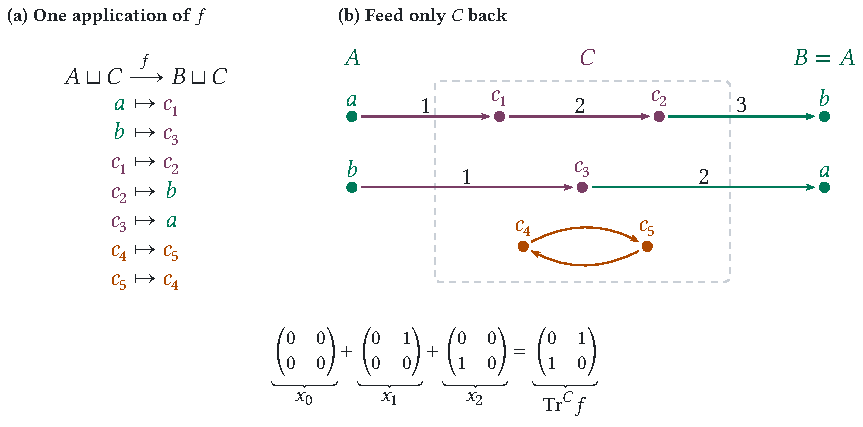
\includegraphics[width=.94\linewidth]{figures/48-paths-cycles.pdf}
\caption{A reversible loop with two external paths and an internal
cycle. The two nonzero exit maps have disjoint domains and their sum
is a swap.}\label{fig:48-paths-cycles}
\Description{The labels A, B and C name basis sets rather than matrix
blocks. Edge labels one, two and three count calls, starting at one.
Two internal points form an inaccessible cycle.}
\end{programfigure}
\begin{theorem}[Finite feedback]\label{thm:total}
For a finite unitary $U:X\oplus Y\to X'\oplus Y$, the exits are
absolutely summable in operator norm. Their sum $L:X\to X'$ is
unitary, and $\sum_k x_k^\dagger x_k=I_X$. The wire equation
$y=Cu+Dy$ has a solution for every $u$. Every solution gives the same
output $Au+By=Lu$.
\end{theorem}
\begin{programfigure}
\begin{minipage}{.43\linewidth}\centering
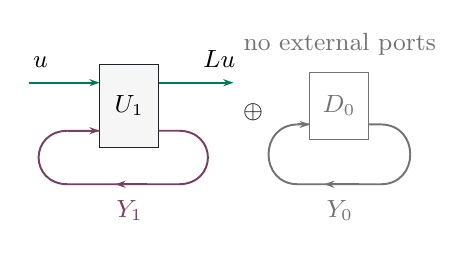
\begin{tikzpicture}[kme circuit,>={Stealth[length=1.3mm,width=.9mm]}]
 \draw[kme gate,fill=ink!4] (.35,.9) rectangle (1.10,1.95);
 \node at (.725,1.43) {$U_1$};
 \draw[flipout,->,line width=.7pt] (-.55,1.72) -- (.35,1.72);
 \draw[flipout,->,line width=.7pt] (1.10,1.72) -- (2.05,1.72);
 \node[above] at (-.40,1.84) {$u$};
 \node[above] at (1.87,1.84) {$Lu$};
 \draw[flipback,line width=.7pt]
(1.10,1.11) -- (1.35,1.11) .. controls (1.85,1.11) and (1.85,.43) ..
(1.35,.43) -- (-.05,.43) .. controls (-.55,.43) and (-.55,1.11) ..
(-.05,1.11) -- (.35,1.11);
 \draw[flipback,->,line width=.7pt] (-.05,1.11) -- (.35,1.11);
 \draw[flipback,->,line width=.7pt] (.95,.43) -- (.55,.43);
 \node[text=flipback,below] at (.73,.30) {$Y_1$};
 \node at (2.30,1.35) {$\oplus$};
 \draw[kme gate,draw=quiet] (3.02,1.0) rectangle (3.76,1.85);
 \node[text=quiet] at (3.39,1.43) {$D_0$};
 \draw[quiet,line width=.7pt]
(3.76,1.19) -- (3.92,1.19) .. controls (4.42,1.19) and (4.42,.43) ..
(3.92,.43) -- (2.87,.43) .. controls (2.37,.43) and (2.37,1.19) ..
(2.87,1.19) -- (3.02,1.19);
 \draw[quiet,->,line width=.7pt] (2.87,1.19) -- (3.02,1.19);
 \draw[quiet,->,line width=.7pt] (3.65,.43) -- (3.20,.43);
 \node[text=quiet,below] at (3.40,.30) {$Y_0$};
 \node[above,text=quiet] at (3.40,1.99) {no external ports};
\end{tikzpicture}
\end{minipage}\hfill
\begin{minipage}{.54\linewidth}\centering
\[
 \begin{aligned}
 \|u\|^2&=\textcolor{flipout}{\|Au\|^2}
+\textcolor{flipback}{\|Cu\|^2},\\[3pt]
 \textcolor{flipback}{\|Cu\|^2}
   &=\textcolor{flipout}{\|BCu\|^2}
+\textcolor{flipback}{\|DCu\|^2},\\[3pt]
 \textcolor{flipback}{\|DCu\|^2}
   &=\textcolor{flipout}{\|BDCu\|^2}
+\textcolor{flipback}{\|D^2Cu\|^2}.
 \end{aligned}
\]
\end{minipage}
\caption{An internal basis change separates $U_1$ from the
unreachable $D_0$. The three norm identities telescope because each
return term supplies the next call.}\label{fig:feedback-proof}
\Description{The accessible unitary body has an external wire and its
own returning wire, while a separate closed component has no external
ports. Three norm identities follow the original input and its next
two continuations.}
\end{programfigure}
\begin{proof}[Proof of Theorem~\ref{thm:total}]
From $U^\dagger U=I$ and $UU^\dagger=I$ we have
\[
A^\dagger A+C^\dagger C=I,\qquad B^\dagger B+D^\dagger D=I,
 \qquad CC^\dagger+DD^\dagger=I.
\]
The middle identity gives $\|Dy\|^2+\|By\|^2=\|y\|^2$. With
$Y_0=\bigcap_{j\ge0}\ker BD^j$, it follows that $D Y_0\subseteq Y_0$
and $D|_{Y_0}$ is isometric. In finite dimension it maps $Y_0$ onto
$Y_0$. Thus $U$ maps $0_X\oplus Y_0$ onto $0_{X'}\oplus Y_0$.
Unitarity maps their orthogonal complements $X\oplus Y_1$ and
$X'\oplus Y_1$ onto one another. Hence $C(X)\subseteq Y_1$,
$D(Y_1)\subseteq Y_1$ for $Y_1=Y_0^\perp$, and $B$ vanishes on $Y_0$.

Write $D_1=D|_{Y_1}$ and $B_1=B|_{Y_1}$. Put $m=\dim Y$. By
Cayley--Hamilton a return vector is invisible exactly when its first
$m$ emissions vanish. If $Y_1=0$, all delayed exits vanish. Otherwise
$m>0$. For a unit $y\in Y_1$, conservation through $m$ calls gives
\[
1-\|D_1^my\|^2=\sum_{j=0}^{m-1}\|BD^jy\|^2>0.
\]
Equality would make every displayed emission zero and hence put $y$
in $Y_0$. On the compact unit sphere of $Y_1$, the continuous
function $y\mapsto\|D_1^my\|$ therefore has a maximum $q<1$. For
$k=pm+r$, $0\le r<m$, norm nonincrease on the remaining $r$ calls
gives $\|D_1^k\|\le\|D_1^m\|^p\|D_1^r\|\le q^p$. This geometric bound
also makes every polynomially weighted exit series converge.
Therefore $\sum\|x_k\|$ is finite and $F=(I-D_1)^{-1}C=\sum_j D_1^jC$
solves the wire equation. Every other solution differs by a vector in
$Y_0$ fixed by $D$, which $B$ kills. The norm identity for
$U(u,Fu)=(Lu,Fu)$ proves that $L$ is an isometry. Since $\dim X=\dim
X'$ it is onto.

To account for the probability, let $T_j=C^\dagger D^{\dagger
j}D^jC$. On a unit input $u$, $\langle u,T_ju\rangle$ is the
probability still inside after call $j+1$. The first block identity
gives $x_0^\dagger x_0=I-T_0$. On later calls the weight that leaves
is exactly the drop in the weight still inside, since
\[
x_{j+1}^\dagger x_{j+1} = C^\dagger D^{\dagger
j}\underbrace{B^\dagger B}_{I-D^\dagger D}D^j C = T_j-T_{j+1}.
\]
Adding through exit $k$ gives $\sum_{j=0}^k x_j^\dagger x_j=I_X-T_k$.
The residual term tends to zero by the decay just proved, giving
total exit probability one even for a body with infinitely many
possible exits.
\end{proof}

For an internal state $w$, write $\mathcal Ow=(BD^jw)_{j\ge0}$ for
the sequence of amplitudes it can still emit. Let
$\mathcal S(z_0,z_1,\ldots)=(z_1,z_2,\ldots)$ be the left shift.
Then $\mathcal OD_1=\mathcal S\mathcal O$ on $Y_1$ says that
advancing a live state drops its first emission from the sequence.
The squared norms of the entries of $\mathcal Ow$ sum to $\|w\|^2$
for $w\in Y_1$, by the same conservation argument as in the proof.
Figure~\ref{fig:71-observe} illustrates this with $B=-4/5$ and
$D=3/5$ on the live direction, and with an independent dead
direction.
\pic{71-observe}{The future emissions of a live state form its
observation tape. Advancing that state shifts the tape by one
position. A dead state has the zero tape. Here $Dv=-v$ is dead but
not fixed; only the fixed subspace $\ker(I-D)$ obstructs the inverse
at phase one.}{The observed live direction loses its first entry when
acted on by the return block.}

\subsection{Eliminating a pattern}\label{app:elim}
\begin{proposition}[Elimination]\label{prop:elim}
Given the expanded table, eliminating its returning basis values in
any order produces a closed iso denoting $L$ in exactly $|\mathcal
B(c)|$ steps. If the original coefficients lie in a subfield of $\C$,
the result has coefficients in that subfield.
\end{proposition}

\begin{proof}[Proof of Proposition~\ref{prop:elim}]
Place the selected return pattern in $Q=\C q$ and put $Y_{\rm
rest}=Y\ominus Q$, the orthogonal complement of $Q$ in $Y$. The
remaining input and output are $E_{\rm in}=X\oplus Y_{\rm rest}$ and
$E_{\rm out}=X'\oplus Y_{\rm rest}$. Grouping those remaining ports
together gives body blocks
\[
 \begin{pmatrix}M&b_q\\c_q&d_q\end{pmatrix},\qquad
M:E_{\rm in}\to E_{\rm out},\quad b_q:Q\to E_{\rm out},\quad
c_q:E_{\rm in}\to Q,\quad d_q\in\C.
\]
Here $d_q=D_{qq}$ is the selected self-entry. For $w=(u,y_{\rm
rest})$, the row $c_q$ gives $c_qw=(Cu)_q+\sum_{r\ne q}D_{qr}y_r$
from the main-text coordinate equation, while $b_q$ collects the
coefficients of $y_q$ in the other outputs. Closing $Q$ asks for a
scalar $\lambda=c_qw+d_q\lambda$ and returns $Mw+b_q\lambda$. When
$d_q\ne1$, solving gives $\lambda=c_qw/(1-d_q)$ and output
$(M+b_qc_q/(1-d_q))w$. When $d_q=1$, its self-entry has norm one, so
every other entry in both its row and column is zero. Hence
$b_q=c_q=0$, any $\lambda$ solves the wire equation, and the output
is $Mw$. These cases are exhaustive. In particular $d_q=-1$ or
$d_q=i$ uses the first branch, with $b_q=c_q=0$; no divergent
geometric series is invoked. Theorem~\ref{thm:total} applied with
these remaining ports external proves unitarity of this intermediate
table in either case.

Figures~\ref{fig:28-sheets} and~\ref{fig:42-elim-flip} apply this
calculation to the scalar rotation and the two return patterns of the
flip.

After one elimination, solving the remaining feedback equations gives
exactly the output of solving all the original equations. Indeed a
simultaneous solution restricts to one of the smaller system, and a
solution of the smaller system can be extended by a solution for $q$
at those incident values. The external value is independent of these
choices by Theorem~\ref{thm:total}. Induct on the number of return
patterns. Each step removes one and uses only field operations with
nonzero denominators. For a phase on the return wire apply the same
argument to the modified unitary. No exchange in the order of a
conditionally convergent series of individual walks is needed.
\end{proof}
\paragraph{Closed sums for the running rotation.}
For \code{guardRound}, both port spaces are $\C$, so the blocks are
scalars: $A=D=t=3/5$, $C=s=4/5$ and $B=-s$. The general exit formula
becomes $x_0=t$ and
$x_{k+1}=(-s)t^ks=-s^2t^k$. To compare adding these amplitudes
with adding their squared magnitudes, follow the first $n$ calls on
unit input. Write $r_n$ for the amplitude still returning,
$\ell_n$ for the sum emitted so far, and $p_n$ for the weight of
those exits when the guard is measured. The geometric sums give
\[
\begin{aligned}
r_n&=st^{n-1},\\
 \ell_n&=t-s^2\sum_{j=0}^{n-2}t^j
=-1+(1+t)t^{n-1},\\ p_n&=t^2+s^4\sum_{j=0}^{n-2}t^{2j}
=1-s^2t^{2(n-1)}.
\end{aligned}
\]
The sums are empty when $n=1$. Table~\ref{tab:rounds} follows the
resulting emissions, residuals and sums. The squared length
$|\ell_n|^2$ can fall and rise as later emissions interfere.
The measured halting weight $p_n$ only increases, because each call
adds a nonnegative probability.
\paragraph{A table and an unknown gate.} There is also no uniform
approximation guarantee for an unknown body given only as a gate. For
a scalar rotation with cosine $t$ the trace is $t-(1-t^2)/(1-t)=-1$
for $-1<t<1$, but at the identity rotation it is $1$. Put a bypass
beside this scalar and the jump is a relative phase detectable by a
Hadamard. A fixed finite circuit built by continuously composing the
supplied body has a continuous response; eliminating a given clause
table can branch on an exact
equality~\cite[Remark~B.1]{FairbanksSelinger25Traces}.



\section{Records, measurement and phase}\label{app:readings}
The counter and measured-loop constructions appear in
Figures~\ref{fig:76-finite-counter-sheet},
\ref{fig:28b-sheets-unrolled} and~\ref{fig:77-measured-sheet} in the
main text. For a common payload
$H=X=X'=Y$, the guard-first transport is
$F_g=\mathsf{factor};\sigma_{H,\mathsf{Qubit}}:H+H\leftrightarrow\kw
{Qubit}\otimes
H$.
It gives $\widehat U_g=\sem{F_g}U\sem{F_g}^{-1}$. For a counter,
$F_{K,g}=d_K^{-1};(I_{[K]}\otimes F_g)$ puts counter, guard and data
in that order, with inverse transport at the output. These are the
equal-payload forms of the general constructions in
Section~\ref{sec:effects}.

Use the Hilbert space $H_{\rm rec}=\ell^2(\N)$ for an exact record,
in the order counter then data. The squared norm of $Ru$ is
$\sum_k\|x_ku\|^2=\|u\|^2$. For the isometric inclusion $J_K:\C^K\to
H_{\rm rec}$ onto the first $K$ labels,
\[
 \|(J_K\otimes I)R_K-R\|
 \ \leq\ \sum_{k\ge K}\big\|\ket{k\bmod K}-\ket k\big\|\,\|x_k\|
 \ \leq\ 2\sum_{k\ge K}\|x_k\| .
\]
For $k\ge K$, the two distinct orthogonal count labels have distance
$\sqrt2\le2$. The bound therefore tends to zero. This argument only
compares the operators produced by finite bodies. The map that folds
all square-summable sequences into residue classes would be
unbounded, as would the map that sums their entries at phase one.

For an input of the form $\ket u\bra v$, tracing the exact record
over its orthonormal basis leaves $\sum_k x_k\ket u\bra v
x_k^\dagger$. Such operators span the input matrix algebra,
giving~\eqref{eq:meas}. For a finite counter put $G_j=\sum_{k\equiv
j\bmod K}x_k$. Discarding that counter instead gives
$\sum_{j<K}G_j\rho G_j^\dagger$. As a result, unequal counts
congruent modulo $K$ retain cross terms. For the Fourier forms, the
coefficient sum is absolutely convergent, and
\[
G_j=\frac1K\sum_{z^K=1}\bar z^{\,j}\Theta(z),\qquad
x_k=\frac1{2\pi}\int_0^{2\pi}
e^{-ik\varphi}\Theta(e^{i\varphi})\,d\varphi .
\]
Expanding $\Theta(z)\rho\Theta(z)^\dagger$ and integrating term by
term removes all unequal indices, proving~\eqref{eq:haar}.

Definition~\ref{def:three-loops} in Section~\ref{sec:effects}
collects the resulting maps on the reference example. For the
classical trace, let
$\theta(\rho,\sigma)=\operatorname{diag}(\rho,\sigma)$ insert the
two operator blocks and let $\varphi$ extract the diagonal output
blocks. Then $\Phi_U=\varphi\circ\chan U\circ\theta$ is the branching
map of Section~\ref{sec:effects}. Its trace on completely positive
trace-nonincreasing maps on finite $C^*$-algebras is the unrolling
$\sum_k x_k\rho
x_k^\dagger$~\cite[Prop.~3.2.17]{AndresMartinez22Thesis}.

\paragraph{Relation to monitored first returns.}
The published test-first loop measures before applying
$U$~\cite[\S~3]{YingFeng10QuantumLoop}. To obtain our body-first
convention when $X'=X$, apply $U$ once before entering it. Let
$\iota_Xu=(u,0)$ and $P=\iota_X\iota_X^\dagger$. For $n\ge1$, the
exit map on call $n$ is
$\iota_X^\dagger U((I-P)U)^{n-1}\iota_X=x_{n-1}:X\to X$. Thus the
monitored-return count includes the initial call and is one more than
our number of returns~\cite[\S~2]{Bourgain14Subspace}.

\section{Agreement and replacement}\label{app:axis}
\begin{proof}[Proof of Theorem~\ref{thm:axis}]
Assume $\meas=\chan L$. For each unit input $u$, test the output on
any $w$ orthogonal to $Lu$. The sum of the nonnegative numbers
$|\langle w,x_ku\rangle|^2$ is zero. Thus $x_ku$ is parallel to $Lu$
for each $k$ and all $u$. Put $V=L^\dagger x_k$. Since $Vu$ lies
along $u$, testing a basis vector $e_i$ gives $Ve_i=\lambda_i e_i$.
To see why the scalar cannot depend on $i$, test two distinct basis
vectors together:
\[
V(e_i+e_j)=
 \underbrace{\lambda_i e_i+\lambda_j e_j}_{\text{by linearity}}
=
 \underbrace{\lambda_{ij}(e_i+e_j)}_{\text{parallel to the input}} .
\]
Comparing the two coordinates gives
$\lambda_i=\lambda_{ij}=\lambda_j$. Hence $V=b_kI$ and $x_k=b_kL$,
including in dimension one where there is only one basis coefficient
to begin with. By absolute convergence, $\sum_k b_k=1$ since $\sum_k
x_k=L\ne0$. By $\sum_k x_k^\dagger x_k=I$, $\sum_k |b_k|^2=1$. The
unit vector $\xi=\sum_k b_k\ket k$ therefore satisfies $R
u=\xi\otimes Lu$. Conversely that factorization implies $\meas=\chan
L$ after tracing out the count; testing each label shows $x_k=\langle
k|\xi\rangle L$.

These conditions imply that $x_0,\ldots,x_m$ span at most a line. If
$m>0$, Cayley--Hamilton writes $D^m$ as a linear combination of
$I,D,\ldots,D^{m-1}$. Since $x_{k+1}=BD^kC$, multiplication by higher
powers shows that every exit after $x_m$ belongs to the span of
$x_1,\ldots,x_m$. If $m=0$, all exits after $x_0$ vanish. Thus the
span of the first $m+1$ exits is the span of all the exits. It cannot
be zero because it contains their unitary sum on the nonzero input.
If it is a line, the same sum $L$ spans it, so $x_k=b_kL$ for each
$k$. Completeness of the exits again gives the unit norm of $\xi$.
This proves all implications.
\end{proof}


\paragraph{Channel contexts.}
Fix the hole type $a\rightsquigarrow b$ and abbreviate it by
$\mathcal H$ to the left of a context judgment. The single hole,
sequential and tensor constructors in Section~\ref{sec:agreement}
have rules
\begin{mathpar}
 \isorule{}{\mathcal H\vdash[-]:a\rightsquigarrow b}
 \and\isorule{h:e\rightsquigarrow c\\\mathcal H\vdash\mathcal
 C:c\rightsquigarrow d}
       {\mathcal H\vdash h;\mathcal C:e\rightsquigarrow d}
 \and\isorule{\mathcal H\vdash\mathcal C:c\rightsquigarrow
 d\\h:d\rightsquigarrow e}
       {\mathcal H\vdash\mathcal C;h:c\rightsquigarrow e}\\
 \isorule{h:e\rightsquigarrow f\\\mathcal H\vdash\mathcal
 C:c\rightsquigarrow d}
       {\mathcal H\vdash h\otimes\mathcal C:e\otimes
       c\rightsquigarrow f\otimes d}
 \and\isorule{\mathcal H\vdash\mathcal C:c\rightsquigarrow
 d\\h:e\rightsquigarrow f}
       {\mathcal H\vdash\mathcal C\otimes h:c\otimes
       e\rightsquigarrow d\otimes f}.
\end{mathpar}
For a finite instrument $(\Psi_j:c\to c_j)_{j\in J}$, meaning
$\Psi_j:\operatorname{End}(\sem c)\to\operatorname{End}(\sem{c_j})$,
the maps are completely positive and their output traces sum to the
input trace. Its case rule is
\[
 \frac{i\in J\quad\mathcal H\vdash\mathcal C:c_i\rightsquigarrow
 d\quad
h_j:c_j\rightsquigarrow d\ (j\ne i)}
      {\mathcal H\vdash\mathsf{case}\bigl(\Psi_i;\mathcal C,
(\Psi_j;h_j)_{j\ne i}\bigr):c\rightsquigarrow d}.
\]
Plugging $h$ into the hole interprets sequencing by channel
composition and tensor by the tensor product of channels. The case
denotes
$\sem{\mathcal C[h]}\circ\Psi_i+\sum_{j\ne i}\sem{h_j}\circ\Psi_j$.
Thus exactly one syntactic occurrence depends on the hole, and each
branch continuation has the channel type stated by the rules. These
contexts can use a hole on one instrument outcome and omit it on the
others. They do not contain iso-level operations on that hole.

\begin{proof}[Proof of Corollary~\ref{cor:replace}]
If $X=0$ then $X'=0$ as well, and there is just one map on the zero
operator space. Now suppose $X\ne0$. On agreement the finite record
has the form $R_Ku=\xi_K\otimes Lu$, where $\xi_K=\sum_k
b_k\ket{k\bmod K}$. Since $R_K$ is an isometry and an input unit
vector exists, $\|\xi_K\|=1$, even if components with equal labels
interfere. Discarding it gives $\chan L$. For the exact record the
equality after discard needs no agreement condition. Channel equality
on data entails equality after tensoring with identity on any finite
reference, since elementary tensor operators span the joint matrix
algebra. Composition with fixed channels, discarding and applying a
fixed instrument on either program therefore preserve equality. For a
measurement-conditioned continuation apply the same argument
separately to each unnormalized outcome and then add if the outcome
is forgotten. This proves the claim by induction over a context built
with these constructors. Conversely, if the channels differ, some
density operator distinguishes them since positive trace-one inputs
span the matrix algebra over $\C$. The two resulting density
operators are distinguished by a spectral projection of their
Hermitian difference. This test is at the output of the empty
context; finite exact isos and tag measurement can implement a
measurement in the chosen eigenbasis.

For delayed discard, use the following separate semantic continuation
calculus. Its ordinary data types are finite, while its opaque
history names may carry countable semantic record spaces. Write
$\Gamma\vdash K:a\Rightarrow b$ for a finite continuation that starts
with ordinary data of type $a$ and the fresh opaque history names in
$\Gamma$, and returns data of type $b$ after consuming all those
names. Each name carries its designated record space. Each branch
$\Psi_j$ of a finite instrument sends operators on $\sem a$ to
operators on $\sem{a_j}$ by a completely positive map. The traces of
these outputs sum to one on each density input. An ordinary channel
is its one-outcome case. For a binder, let $R:\sem a\to H\otimes\sem
d$ be a recording isometry. Its history name $g$ has space $H$. The
caller rules are
\begin{mathpar}
 \isorule{}{\varnothing\vdash\mathsf{return}:a\Rightarrow a}
 \and\isorule{\Gamma\vdash K_j:a_j\Rightarrow b\quad(j\in J)}
    {\Gamma\vdash\mathsf{case}\ (\Psi_j;K_j)_{j\in J}:a\Rightarrow
    b}\\
 \isorule{\Gamma\vdash K:a\Rightarrow b\quad h\notin\Gamma}
    {\Gamma,h\vdash\mathsf{drop}\ h;K:a\Rightarrow b}
 \and\isorule{\Gamma,g\vdash K:d\Rightarrow b\quad g\notin\Gamma}
    {\Gamma\vdash\mathsf{record}\ g=R\ \mathsf{in}\ K:a\Rightarrow
    b}.
\end{mathpar}
Bound names are chosen fresh throughout the finite derivation by
renaming. For an ordering of the live names, let $H_\Gamma$ be their
tensor product and $I_\Gamma$ its identity. The semantics maps
trace-class operators on $H_\Gamma\otimes\sem a$ to operators on
$\sem b$. With canonical reassociations and permutations of named
factors understood, its equations are
\[
\begin{aligned}
 \sem{\mathsf{return}}&=\mathrm{id},\\
 \sem{\mathsf{case}\ (\Psi_j;K_j)_{j\in J}}
    &=\sum_{j\in J}\sem{K_j}\circ(\mathcal
    E_{I_\Gamma}\otimes\Psi_j),\\
 \sem{\mathsf{drop}\ h;K}&=\sem K\circ\tr_h,\\
 \sem{\mathsf{record}\ g=R\ \mathsf{in}\ K}
    &=\sem K\circ\mathcal E_{I_\Gamma\otimes R}.
\end{aligned}
\]
The instrument selects a continuation by its classical outcome and
passes all live names to that continuation. A binder adds its new
record, and a drop traces out just the named factor. Only the empty
history context can return, so each returning branch drops every live
name exactly once. For $K_h$ starting with a distinguished $h$, fresh
for every internal record binder, delete its drops to obtain $K$,
leaving all other binders and drops in place. The rules show that $K$
is well typed with $h$ removed. On each returning branch and for any
joint trace-class input $\tau$,
\[
                  \sem{K_h}(\tau)=\sem K(\tr_h\tau).
\]
For a drop it is the definition. For an ordinary operation $\Psi$
before the drop, use
$\tr_h((\mathcal E_{I_h}\otimes\Psi)(\tau))=\Psi(\tr_h\tau)$, by
taking the partial trace in a basis of $h$. This holds for each
subnormalized instrument outcome, and tensoring with a reference
leaves it valid. Nested recording is an isometry on the ordinary data
and the new record, with the older name carried by the identity.
Partial traces over distinct names commute at their eliminations.
Induction over sequencing, measurement branches and nested bindings
proves the formula. Consequently a recording atom $R$ followed by
$K_h$ may be
replaced by its marginal channel $\rho\mapsto\tr_H(R\rho R^\dagger)$
followed by $K$. When $R$ is the exact exit record of our body
$\beta$, this marginal is $\mathsf{while}_c\,\beta$
by~\eqref{eq:meas}.
Under agreement it may also be replaced by the embedded coherent iso.
A finite clock has its own marginal and does not in general admit the
unconditional exact-record replacement. If a caller is a limit of
increasing finite executions with subnormalized outputs, the same
pathwise identities preserve its lost trace under that limit. This
last observation assumes such a semantics; general recursive callers
are outside the finite grammar.
\end{proof}

\paragraph{Why one finite clock does not suffice.}
The output interface matters. If a caller reads the count, even a
fixed count independent of the data is an observable output.
Conversely, a finite clock may hide a failure of agreement. Use the
permutation $E0\mapsto E0$ and $E1\mapsto Bq_1\mapsto\cdots\mapsto
Bq_K\mapsto E1$, with $K$ distinct return values $q_1,\ldots,q_K$.
Its only nonzero exits are $x_0=\ket0\bra0$ and $x_K=\ket1\bra1$. The
$K$-clock assigns label $0$ to both exits. Ignoring it preserves
$\ket+=(\ket0+\ket1)/\sqrt2$, whereas a measurement on every return
dephases $\ket+$ in that basis. Checking just this clock would accept
the replacement incorrectly.

\section{The derivative and its average}\label{app:deriv}
\begin{proof}[Proof of Theorem~\ref{thm:deriv}]
Work on $Y_1$. The geometric bound in Theorem~\ref{thm:total} gives
an open disk of radius greater than one on which $F_z$ and
$\Theta(z)$ are analytic. Empty live space gives $F_z=0$. The
identity $F_z=C+zD_1F_z$ says
\[
U_1(u,zF_z u)=(\Theta(z)u,F_z u).
\]
Use the wire equation twice, first at $(v,w)$ and then at $(u,z)$.
Because $U_1:X\oplus Y_1\to X'\oplus Y_1$ preserves inner products,
the inner product of the inputs equals that of the outputs. With the
inner product linear in its second argument, the two sides are
\[
 \underbrace{\langle v,u\rangle+\bar w z\langle
 F_wv,F_zu\rangle}_{\text{external and returning inputs}}
=
 \underbrace{\langle\Theta(w)v,\Theta(z)u\rangle+\langle
 F_wv,F_zu\rangle}_{\text{external and returning outputs}} .
\]
Collecting terms gives $I-\Theta(w)^\dagger\Theta(z)=(1-\bar w
z)F_w^\dagger F_z$. Keep $w$ fixed on the unit circle and
differentiate with respect to $z$. At $z=w$ the factor $1-\bar w w$
is zero, so the term containing $F'_z$ vanishes. The remaining
equality is $\Theta(w)^\dagger\Theta'(w)=\bar w F_w^\dagger F_w$. Now
put $w=e^{i\varphi}$. The angular derivative multiplies $\Theta'(w)$
by $iw$, giving $Q(w)=F_w^\dagger F_w$ as claimed.

By the telescope in Appendix~\ref{app:total},
$\sum_{k=1}^p k x_k^\dagger x_k=\sum_{j=0}^{p-1}T_j-pT_p$. Geometric
decay makes $pT_p\to0$. Thus $N=\sum_j T_j$. In $F_z^\dagger F_z$ the
terms at $m,n$ have factor $z^{n-m}$ on the unit circle. As in
Figure~\ref{fig:phase-grid}, integration keeps only the cells where
$m=n$. Uniform absolute convergence permits this termwise
integration, leaving $\sum_j T_j$. This gives the phase average. For
the trace of $N$, cyclicity changes the summand $\tr T_j$ into
$\tr(D_1^j CC^\dagger D_1^{\dagger j})$. From the $Y_1$ output block
of $U_1U_1^\dagger=I_{X'\oplus Y_1}$ we have
$CC^\dagger=I-D_1D_1^\dagger$. The partial sum once again telescopes,
\[
 \sum_{j=0}^{p-1}D_1^j CC^\dagger D_1^{\dagger j}
=I_{Y_1}-D_1^pD_1^{\dagger p}\ \longrightarrow I_{Y_1}.
\]
Thus $\tr N=\dim Y_1$. On each unit input $u$ the measured
probability of exit $k$ is $\|x_k u\|^2$, so its mean count is
$\sum_k k\|x_ku\|^2=\langle u,Nu\rangle$.
\end{proof}



For the monitored first-return convention the generating function is
$z\Theta(z)$, whose relative derivative is $I+Q(z)$. Its mean number
of calls is therefore $1+\langle u,Nu\rangle$~\cite[\S~3,
Eq.~(8)]{Bourgain14Subspace}. A phase on the return tag is an
ordinary iso, so forming this family requires no counter or guard
measurement.


\paragraph{Phase invariance and agreement.}
On a nonempty external type, the phase family also characterizes
agreement. If every exit is $x_k=b_kL$, then
$\Theta(z)=f(z)L$ with $|f(z)|=1$ on the circle, so every marking
phase gives the same data channel. Conversely, if those channels are
all equal, they equal $\chan L$ because $\Theta(1)=L$. Their average
is $\meas$ by~\eqref{eq:haar}, so
$\meas=\chan L$.
Thus agreement says exactly when changing the return phase leaves the
data channel unchanged.

\setcounter{topnumber}{6}
\setcounter{bottomnumber}{5}
\setcounter{totalnumber}{8}
\renewcommand{\floatpagefraction}{.55}
\renewcommand{\textfraction}{.05}
\section{Clause programs and their observations}\label{app:programs}
Many small loop bodies can be written as two clauses with a variable
for the payload. We give their definitions here so that one can
reproduce each diagram directly from an iso. Each program closes its
returning summand with \kw{trace}. We abbreviate \kw{exit} and
\kw{back} by $E$ and $B$ in this section's source equations. In these
equations $B$ is an injection tag; a matrix block appears only in a
denotational equation. In executable types, \code{x} spells tensor
product, and a coefficient \code{(a :+ b)} denotes $a+ib$ for real
$a,b$.

\paragraph{Two scalar loops in sequence.}
Use two copies of the scalar guard rotation, with $t=3/5$ and
$s=4/5$. Their separate returns each receive the phase $z$, and their
external ports connect in sequence. The responses therefore multiply
to $f(z)^2$, where $f(z)=(t-z)/(1-tz)$. Figure~\ref{fig:72-peel}
gives both this cascade and its single-round matrix $W$ on $\mathbb
C\oplus(\mathbb C\oplus\mathbb C)$. Multiplying its blocks, or
solving its two return equations, gives the same $f(z)^2$. The
columns of $W$ give the following three clauses; its two returning
basis values are \code{back 0} and \code{back 1}.
\par\noindent\begin{minipage}{\linewidth}
\begin{lstlisting}
round twoSections : Unit + Qubit = {
  exit unit <-> [9/25 . exit unit + 4/5 . back 0 + 12/25 . back 1];
  back 0 <-> [-12/25 . exit unit + 3/5 . back 0 + -16/25 . back 1];
  back 1 <-> [-4/5 . exit unit + 3/5 . back 1]
}

trace twoSections on unit
\end{lstlisting}
\end{minipage}\par
The command returns $\ket*$, since $f(1)^2=1$. A period-two clock
also returns label $0$: both $f(1)^2$ and $f(-1)^2$ are one, so the
odd residue sum is zero.

{\renewcommand{\picdir}{figures}\pic{72-peel}{Two specified scalar
sections give response $f(z)^2$. The numerical matrix is the open
body of this cascade in external-first order.}{Two rotation loops and
their rational three-by-three open body.}}
Now carry data $u$ unchanged through both sections and apply a gate
$L$ once on the final external output. As
Figure~\ref{fig:81-axis-shape} shows, this amounts to tensoring the
internal evolution with the identity on the data. The response is
$f(z)^2L$. Every exit coefficient multiplies the same $L$, so
dropping the count preserves the data channel by
Theorem~\ref{thm:axis}. On the unit circle $|f|=1$, hence the
relative derivative of the squared scalar response is twice that of
one section. Its phase average gives mean count two, as expected from
the mean of one for each rotation. Changing coordinates on the
internal space or adjoining an inaccessible summand leaves the exits
unchanged.
{\renewcommand{\picdir}{figures}\pic{81-axis-shape}{Tensor the
specified two-section body with the data identity and apply $L$ on
its external output. This constructed body passes agreement and has
mean count two.}{The two-section example carries data unchanged
inside and applies one gate on exit.}}

\subsection{A flip on every call}\label{app:flip}
For a loop that also transforms a payload on every call, take a guard
and a data qubit, apply $R_\theta$ to the guard and the data flip
$J=\mathsf X$ to the data, and close the returning summand. This is
more structure than the scalar loop of the main text needs, but it
gives a second example where measured and coherent outputs differ.
The following source binds the data in each clause before applying
its gate.
\par\noindent\begin{minipage}{\linewidth}
\begin{lstlisting}
X :: Qubit <-> Qubit
X = { 0 <-> 1; 1 <-> 0 }

round flipRound : Qubit + Qubit = {
  exit x <-> let y = X x in [ 3/5 . exit y + 4/5 . back y];
  back x <-> let y = X x in [-4/5 . exit y + 3/5 . back y]
}
\end{lstlisting}
\end{minipage}\par
The first definition names the data gate $\mathsf X$ inside the box
in Figure~\ref{fig:flip-circuit}. On input \code{exit 0} the first
clause binds $x=0$, so \code{let y = X x} binds $y=1$. Each dot
scales a tagged output, and the brackets form their superposition.
The coefficients $3/5$ and $4/5$ are the first column of $R_\theta$,
since \kw{exit} means that the guard enters at $0$. Following
\code{back 1} into the second clause flips the data once more and
uses the other column, with coefficients $-4/5$ and $3/5$. This is
where the second call acquired its minus sign. With the guard first
and the data second, Figure~\ref{fig:38-clause-table} is the matrix
of $R_\theta\otimes\mathsf X$.




\begin{programfigure}
\centering
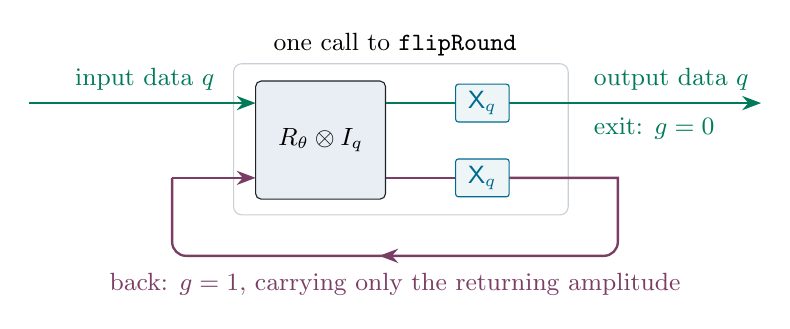
\begin{tikzpicture}[kme circuit,>=Stealth]
  \draw[draw=hairline,fill=white,rounded corners=3pt] (-2.05,-.82)
  rectangle (2.20,1.10);
  \node[anchor=south] at (0,1.12) {one call to \code{flipRound}};
  \draw[draw=ink,fill=accentsoft,rounded corners=2pt] (-1.77,-.62)
  rectangle (-.12,.88);
  \node at (-.945,.13) {$R_\theta\otimes I_q$};
  \draw[flipout,line width=.85pt,->] (-4.65,.60) -- (-1.77,.60);
  \draw[flipout,line width=.85pt] (-.12,.60) -- (.77,.60);
  \draw[flipout,line width=.85pt,->] (1.45,.60) -- (4.65,.60);
  \draw[flipback,line width=.85pt] (-.12,-.35) -- (.77,-.35);
  \draw[flipback,line width=.85pt] (1.45,-.35) -- (2.83,-.35)
    [rounded corners=5pt] -- (2.83,-1.34) -- (-2.83,-1.34) --
    (-2.83,-.35);
  \draw[flipback,line width=.85pt,->] (-2.83,-.35) -- (-1.77,-.35);
  \draw[flipback,line width=.85pt,->] (.20,-1.34) -- (-.20,-1.34);
  \foreach \yy in {.60,-.35}{
    \draw[draw=equalcount,fill=equalcount!7,rounded corners=1pt]
    (.77,\yy-.24) rectangle (1.45,\yy+.24);
    \node[text=equalcount] at (1.11,\yy) {$\mathsf X_q$};
  }
  \node[anchor=south east,text=flipout] at (-2.22,.69) {input data
  $q$};
  \node[anchor=south west,text=flipout] at (2.45,.69) {output data
  $q$};
  \node[anchor=north west,text=flipout] at (2.45,.49) {exit: $g=0$};
  \node[below,text=flipback] at (0,-1.48) {back: $g=1$, carrying only
  the returning amplitude};
\end{tikzpicture}
\par\medskip
{\renewcommand{\arraystretch}{1.55}\setlength{\tabcolsep}{11pt}
\begin{tabular}{@{}clll@{}}
\toprule
Call & Component entering this call & \textcolor{flipout}{Leaves the
loop} & \textcolor{flipback}{Continues to the next call}\\
\midrule
1 & \textcolor{flipout}{$\ket{00}$} & $\tfrac35\ket{01}$ &
$\tfrac45\ket{11}$\\ 2 & \textcolor{flipback}{$\tfrac45\ket{11}$} &
$-\tfrac{16}{25}\ket{00}$ & $\tfrac{12}{25}\ket{10}$\\ 3 &
\textcolor{flipback}{$\tfrac{12}{25}\ket{10}$} &
$-\tfrac{48}{125}\ket{01}$ & $\tfrac{36}{125}\ket{11}$\\
\bottomrule
\end{tabular}}
\caption{The coherent loop connects the body's returning output to
its returning input. The two ports are alternative guard values, each
carrying the same data qubit $q$. Both alternatives apply $\mathsf
X_q$; this data gate commutes with the guard rotation. The table
starts at $\ket{00}$ and writes joint states $\ket{gq}$, with guard
first. Emitted components do not enter a later row; only the last
column does. No guard measurement is made
here.}\label{fig:flip-circuit}
\Description{A sum-feedback diagram shows a guard rotation followed
by a data flip on each summand. The returning summand is connected
around the body. A spaced three-row table separates emitted and
continuing joint components.}
\end{programfigure}
{\renewcommand{\picdir}{figures}\pic{38-clause-table}{The four
columns of the payload-flipping body, in external-first order. This
is $R_\theta\otimes\mathsf X$.}{An expanded four-clause matrix has
orthonormal input columns.}}
{\renewcommand{\picdir}{figures}\pic{05-flip-walk}{On input $\ket0$,
the left panel adds exit amplitudes in the data space. The right
panel keeps the exit rounds distinct and plots their probabilities.
Calls are numbered from one.}{The amplitude path approaches minus the
input. The probability bars are nonnegative and the remaining weight
decreases at every round.}}


\paragraph{Which exits does the flip add?}
Put $t=3/5$ and $s=4/5$. The two clauses of \code{flipRound} give
$A=t\mathsf X$, $C=s\mathsf X$ on entry and $B=-s\mathsf X$,
$D=t\mathsf X$ on return. Hence $x_0=t\mathsf X$ and $x_1=BC=-s^2 I$.
The data flips twice before that second exit. In general
$x_{k+1}=-s^2t^k\mathsf X^{k+2}$. Grouping equal data gates gives two
ordinary geometric series,
\[
 \underbrace{t-s^2t\sum_{j\ge0}t^{2j}}_{\text{coefficient of }\mathsf
 X}=0,
 \qquad
 \underbrace{-s^2\sum_{j\ge0}t^{2j}}_{\text{coefficient of }I}=-1,
 \qquad s^2=1-t^2 .
\]
Thus the whole coherent loop returns $-u$. In particular it can never
return data $1$ on input $0$. With an exact count the exits that
return $0$ on this input have odd counts, with amplitudes
$-s^2,-s^2t^2,\ldots$. Their squared magnitudes sum to
$s^4/(1-t^4)=8/17$. The complementary probability $9/17$ goes to $1$.
These are the two observations in Figure~\ref{fig:05-flip-walk}.
\pic{47-parity-clock-note}{For the flip, folding by parity cancels
all even counts as amplitudes. Measurement of an exact count has
positive probability at every count.}{A cyclic two-state counter
groups all emissions into their even and odd bins.}



The numerical elimination also gives a finite calculation of this
loop. Unlike \code{guardRound}, it has two returning basis patterns.
Figure~\ref{fig:42-elim-flip} in the main text gives both elimination
steps and every new coefficient.
\Needspace{10\baselineskip}
The first substitution in Figure~\ref{fig:42-elim-flip} removes
\code{back 0} and leaves coefficient $(3/5)^2=9/25$ on the remaining
return amplitude $y_1$. It also changes the coefficient of $y_1$ in
external output $v_1$ to $(3/5)(-4/5)=-12/25$. On external basis
input $0$, an amplitude $4/5$ enters this remaining return pattern.
Solving its scalar wire equation gives the two entries in that output
column:
\[
 \begin{aligned}
 \text{on data }0:\quad &\frac{(4/5)(-4/5)}{1-9/25}=-1,\\
 \text{on data }1:\quad &\frac35+\frac{(4/5)(-12/25)}{1-9/25}=0 .
 \end{aligned}
\]
Interchanging the data bits gives the other column. Thus the finite
rewrite produces the same $-I$ that we obtained by adding the exits
round by round.


\FloatBarrier

\paragraph{Moving the flip to the exit.}
A variant that passes the agreement test has the circuit in
Figure~\ref{fig:guard-circuit}. In the ground clauses, the bit after
\kw{exit} is the flipped input bit and the bit after \kw{back} is the
input itself.
\par\noindent\begin{minipage}{\linewidth}
\begin{lstlisting}
round flipOnExit : Qubit + Qubit = {
  exit 0 <-> [ 3/5 . exit 1 + 4/5 . back 0];
  exit 1 <-> [ 3/5 . exit 0 + 4/5 . back 1];
  back 0 <-> [-4/5 . exit 1 + 3/5 . back 0];
  back 1 <-> [-4/5 . exit 0 + 3/5 . back 1]
}
\end{lstlisting}
\end{minipage}\par
\begin{programfigure}
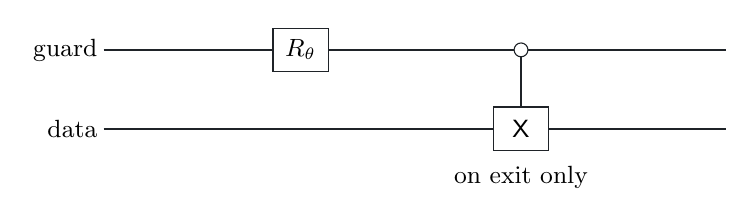
\begin{tikzpicture}[kme circuit]
\draw[kme wire] (0,1) node[left]{guard} -- (7.9,1);
\draw[kme wire] (0,0) node[left]{data} -- (7.9,0);
\draw[kme wire] (5.30,0)--(5.30,1);
\node[kme open] at (5.30,1) {};
\node[kme gate] at (2.5,1) {$R_\theta$};
\node[kme gate] at (5.30,0) {$\mathsf X$};
\node[anchor=north,font=\small] at (5.30,-.40) {on exit only};
\end{tikzpicture}
\caption{The same rotation as in \code{flipRound}, with the flip
controlled on the outgoing guard being $0$. A returning component
keeps its data. Whichever round exits, that component of the data is
flipped exactly once.}\label{fig:guard-circuit}
\Description{The guard passes through the rotation and then controls
a data flip with an open control on zero.}
\end{programfigure}
Running \code{trace flipOnExit on 0} gives $-\ket1$. The measured
command \code{while flipOnExit on 0} gives $\ket1\bra1$. Its exits
are $(3/5)\mathsf X$ at count zero and $-(16/25)(3/5)^{k-1}\mathsf X$
at counts $k\ge1$, using the scalar coefficients calculated in
Section~\ref{sec:trace}. Every exit is proportional to $\mathsf X$,
so agreement holds on every input, including one entangled with a
reference. The coherent completion is $-\mathsf X$.


\paragraph{Rotation with a data iso.}
For $c=\cos\theta$, $s=\sin\theta$ and an iso $M:a\leftrightarrow a$,
define $\mathsf{rotbody}(\theta,M):a+a\leftrightarrow a+a$ by the
clauses
\[
\begin{aligned}
E\,x&\leftrightarrow\mathsf{let}\ y=M\,x\ \mathsf{in}\
c\,E\,y+s\,B\,y,\\ B\,x&\leftrightarrow\mathsf{let}\ y=M\,x\
\mathsf{in}\ -s\,E\,y+c\,B\,y .
\end{aligned}
\]
The notation is a schema for named first-order isos, not a
higher-order value. Putting $M=\mathsf X$ gives the four ground
instances of the flip. For $|c|<1$ its exits are $cM$ and
$-s^2c^kM^{k+2}$. Summing them gives
\[
f_\theta(M)=M(cI-M)(I-cM)^{-1}.
\]
On an eigenvector of $M$ with eigenvalue $w$, the equation
$f_\theta(w)=1$ reduces to $w^2-2cw+1=0$, while $f_\theta(w)=-1$
reduces to $w^2=1$. Hence taking $M$ to be the real rotation of angle
$-\theta$ gives the identity. When $|c|=1$, the guard never enters
and the immediate exit gives the same conclusion for that rotation.
Taking $M=\mathsf X$ gives $-I$ for $|c|<1$.

Here is the inverse-rotation instance at $c=3/5$, including its
invocation. The first declaration supplies $M=R_{-\theta}$; the
second applies it locally on each call.
\par\noindent\begin{minipage}{\linewidth}
\begin{lstlisting}
inverseRotation :: Qubit <-> Qubit
inverseRotation = {
  0 <-> [3/5 . 0 + -4/5 . 1];
  1 <-> [4/5 . 0 + 3/5 . 1]
}

round undoRound : Qubit + Qubit = {
  exit x <-> let y = inverseRotation x in
    [3/5 . exit y + 4/5 . back y];
  back x <-> let y = inverseRotation x in
    [-4/5 . exit y + 3/5 . back y]
}

trace undoRound on 0
\end{lstlisting}
\end{minipage}\par
The command returns $\ket0$. On an arbitrary vector the completed
gate is $I$, as the eigenvalue calculation shows. The measured loop
need not agree: on $\ket+$ it gives
$\tfrac1{650}\left(\begin{smallmatrix}349&-107\\-107&301\end
{smallmatrix}\right)$
rather than $\ket+\bra+$. The cancellation giving the coherent
identity takes place between exits on different rounds.


\paragraph{A guard whose two payloads differ.}
A tag test need not be a measurement of a qubit register beside an
unchanged data type. Take the two external patterns $0,1$ and just
one return pattern $*$. The body below is the three-cycle of
monitored recurrence, with its basis
relabeled~\cite[Example~3.1]{Bourgain14Subspace}. It binds no history
variable.
\par\noindent\begin{minipage}{\linewidth}
\begin{lstlisting}
cycle3 :: (Qubit + Unit) <-> (Qubit + Unit)
cycle3 = {
  left (left unit)  <-> right unit;
  left (right unit) <-> left (left unit);
  right unit        <-> left (right unit)
}
\end{lstlisting}
\end{minipage}\par
Input $1$ exits immediately as $0$, whereas input $0$ returns once
and exits as $1$. Thus $x_0=\ket0\bra1$, $x_1=\ket1\bra0$, and all
later exits vanish. Calling \kw{trace} on this iso gives the flip
$\mathsf X$, so $\ket+$ returns unchanged. Calling \kw{count} with
period two gives $(\ket0\ket0+\ket1\ket1)/\sqrt2$, with counter
first. Calling \kw{while} on the very same iso returns $I/2$ on that
input. The two exit vectors on $\ket+$ have zero inner product, but
they are values of the data we retain. Coherent feedback still
preserves the terms $\ket0\!\bra1$ and $\ket1\!\bra0$ between them. A
separate ignored count removes these terms because it gives the two
data vectors different orthogonal labels. Thus distinguishable data
values alone do not make recording the round harmless.


\paragraph{A cycle, a reflection and a phase.}
The $\mathsf{cycle3}$ program just defined gives the data flip after
closing its one return pattern. One may add a dead pattern with its
own identity clause, obtaining the same flip on a two-pattern return
type. A body with no data can instead be the reflection
$E\,*\leftrightarrow t\,E\,*+s\,B\,*$, $B\,*\leftrightarrow
s\,E\,*-t\,B\,*$ at $t=3/5,s=4/5$. Its immediate exit is $t$, and its
delayed sum is $s^2/(1+t)$. They add to $1$.
\par\noindent\begin{minipage}{\linewidth}
\begin{lstlisting}
round reflection : Unit + Unit = {
  exit unit <-> [3/5 . exit unit + 4/5 . back unit];
  back unit <-> [4/5 . exit unit + -3/5 . back unit]
}

trace reflection on unit
\end{lstlisting}
\end{minipage}\par
This command returns $\ket*$. The measured loop also returns the sole
external value with probability one. Its parity record is
$\ket1\otimes\ket*$: the even exits cancel and the odd exits add to
one. This reflection and \code{guardRound} therefore have the same
measured data output but opposite coherent phases.
{\renewcommand{\picdir}{figures}
\pic{12-axis}{The scalar reflection gives the same data under
measurement or coherent feedback. For the three-cycle, measuring
yields $I/2$ while coherent feedback returns the pure state
$\ket+$.}{Two panels compare the real scalar reflection amplitudes to
the three-cycle on a superposed input. The reflection rows are
vertically offset for legibility.}}



For another example, take the four permutation clauses
\[
E0\mapsto E0,\quad E1\mapsto B1,\quad B0\mapsto B0,\quad B1\mapsto E1
.
\]
Multiply every output by $g$ with $|g|=1$. Input $0$ receives one
factor of $g$ and input $1$ receives two, giving
$\operatorname{diag}(g,g^2)$. The one-call channel is unchanged by
this common phase but the loop channel in general changes. Placing a
phase $z$ on the \emph{returning} outputs alone instead gives
$\operatorname{diag}(1,z)$. The markings occur in different places,
but at $z=g$ their completions differ only by the global factor $g$.
They therefore give the same data channel for this permutation. That
channel can still differ from the unmarked identity channel.

The following two programs instantiate $g=z=i$, written \code{(0 :+
1)} in executable syntax. Both use the exact input
$3\ket0/5+4\ket1/5$.
\par\noindent\begin{minipage}{\linewidth}
\begin{lstlisting}
round unmarked : Qubit + Qubit = {
  exit 0 <-> exit 0;
  exit 1 <-> back 1;
  back 0 <-> back 0;
  back 1 <-> exit 1
}

round wholePhase : Qubit + Qubit = {
  exit 0 <-> (0 :+ 1) . exit 0;
  exit 1 <-> (0 :+ 1) . back 1;
  back 0 <-> (0 :+ 1) . back 0;
  back 1 <-> (0 :+ 1) . exit 1
}

trace wholePhase on 3/5 . 0 + 4/5 . 1
\end{lstlisting}
\end{minipage}\par
This invocation returns $3i\ket0/5-4\ket1/5$.
\par\noindent\begin{minipage}{\linewidth}
\begin{lstlisting}
round returnPhase : Qubit + Qubit = {
  exit 0 <-> exit 0;
  exit 1 <-> (0 :+ 1) . back 1;
  back 0 <-> (0 :+ 1) . back 0;
  back 1 <-> exit 1
}

trace returnPhase on 3/5 . 0 + 4/5 . 1
\end{lstlisting}
\end{minipage}\par
The second returns $3\ket0/5+4i\ket1/5$. Multiplying it by $i$ gives
the first output, so their density operators agree.

\paragraph{Kickback with a returned ancilla.}
Let $J=\mathsf X$, $H$ be Hadamard, $G=HJ$, and $\Pi_\pm=(I\pm J)/2$.
Use $\mathsf{rotbody}(\pi/4,M)$ with ancilla and data as payload,
where $M=G\otimes\Pi_++JG\otimes\Pi_-$. In iso syntax this $M$ is an
operation controlled in the $J$ basis of the data: change that basis
with $H$, apply $G$ or $JG$ to the ancilla according to the resulting
tag, then undo the basis change. In the first sector $G^2=\sqrt2G-I$,
so $f_{\pi/4}(G)=I$. In the second $(JG)^2=I$, so $f_{\pi/4}(JG)=-I$.
The completed loop is $I\otimes(\Pi_+-\Pi_-)=I\otimes J$. Thus it
returns the ancilla on arbitrary joint inputs, not only on a selected
initialization.

In the basis of the two payload bits, the projector sum gives
\[
M\ket{0,d}=\frac{\ket{0,1-d}-\ket{1,1-d}}{\sqrt2},\qquad
M\ket{1,d}=\frac{\ket{0,d}+\ket{1,d}}{\sqrt2}.
\]
The data bit flips in the first case and stays in the second.
Expanding the guard rotation now gives the clauses below. Each
nonzero coefficient of $M$ is $\pm1/\sqrt2$, and the guard
contributes another $1/\sqrt2$, leaving only coefficients $\pm1/2$.
Thus no rounded Hadamard coefficient is needed in this source.
\par\noindent\begin{minipage}{\linewidth}
\begin{lstlisting}
round kickbackExact : (Qubit x Qubit) + (Qubit x Qubit) = {
  exit <0, 0> <-> [1/2 . exit <0, 1> + -1/2 . exit <1, 1>
                + 1/2 . back <0, 1> + -1/2 . back <1, 1>];
  exit <0, 1> <-> [1/2 . exit <0, 0> + -1/2 . exit <1, 0>
                + 1/2 . back <0, 0> + -1/2 . back <1, 0>];
  exit <1, 0> <-> [1/2 . exit <0, 0> + 1/2 . exit <1, 0>
                + 1/2 . back <0, 0> + 1/2 . back <1, 0>];
  exit <1, 1> <-> [1/2 . exit <0, 1> + 1/2 . exit <1, 1>
                + 1/2 . back <0, 1> + 1/2 . back <1, 1>];
  back <0, 0> <-> [-1/2 . exit <0, 1> + 1/2 . exit <1, 1>
                + 1/2 . back <0, 1> + -1/2 . back <1, 1>];
  back <0, 1> <-> [-1/2 . exit <0, 0> + 1/2 . exit <1, 0>
                + 1/2 . back <0, 0> + -1/2 . back <1, 0>];
  back <1, 0> <-> [-1/2 . exit <0, 0> + -1/2 . exit <1, 0>
                + 1/2 . back <0, 0> + 1/2 . back <1, 0>];
  back <1, 1> <-> [-1/2 . exit <0, 1> + -1/2 . exit <1, 1>
                + 1/2 . back <0, 1> + 1/2 . back <1, 1>]
}

trace kickbackExact on 3/5 . <0, 0> + 4/5 . <1, 1>
\end{lstlisting}
\end{minipage}\par
The input is entangled between ancilla and data. Its output is
$3\ket{0,1}/5+4\ket{1,0}/5$, exactly the result of applying $J$ to
the second component. The same identity on arbitrary joint inputs
follows from the two-sector calculation above.


\subsection{Other retained histories}\label{app:record-examples}
In the map example of \emph{From Symmetric Pattern-Matching to
Quantum Control}, the iso argument $g:a\leftrightarrow b$ is applied
to a head and the recursive iso $f$ to the tail. In the source's list
notation the two clauses read~\cite[\S~4]{SabryValironVizzotto18}
\[
 \begin{aligned}
 []&\leftrightarrow [],\\
h:t&\leftrightarrow\ \mathsf{let}\ x=g\,h\ \mathsf{in}\
              \mathsf{let}\ y=f\,t\ \mathsf{in}\ x:y .
 \end{aligned}
\]
If $g$ is Hadamard and the input has length two, every output of the
recursion still has length two. A superposition of input lengths two
and three likewise produces two components that can be distinguished
by length alone. This explains how a reversible program can retain
the depth of its recursion without ever measuring it. The cyclic
register in~\eqref{eq:count} lets us make the same distinction, up to
its period, on a body whose input need not contain a list.

An exact record may also be carried by orthogonal time slots: one
tick of delay on the return wire puts $x_0u,x_1u,\ldots$ in
consecutive output slots~\cite[\S~3.4]{AndresMartinez22Thesis}. In
the common-clock halting construction, a common post-halt ancilla
sequence likewise distinguishes halt times at a fixed observation
time. The original model also allows different ancilla sequences
across branches, which can restore interference
later~\cite{LindenPopescu98Halting}. Our exact record requires
distinct halt times to remain orthogonal at observation.
Appendix~\ref{sec:ring} gives the corresponding short-pulse and
single-frequency experiments.

\paragraph{A case inside or outside feedback.}
Let $\theta$ have $\cos\theta=t=3/5$ and rotate the guard alone. A
phase $z$ on the returning output gives $\theta_0(z)=(t-z)/(1-tz)$ by
summation of the scalar exits. The case
$I\oplus\mathsf{trace}(\mathsf{rotbody}(\theta,I);(I\oplus zI))$ on a
reference qubit therefore denotes
$\operatorname{diag}(1,\theta_0(z))$. If instead the data bit selects
the phase on a return \emph{inside} the guard rotation, the two data
sectors get $\theta_0(1)$ and $\theta_0(z)$. The result is
$\operatorname{diag}(-1,\theta_0(z))$. The bypass in the first
program makes no visit to the loop, whereas both sectors in the
second visit it. At $z=i$, the two open bodies are the following
literal programs. A factor \code{(0 :+ 1)} contributes $i$ only to a
returning output.
\par\noindent\begin{minipage}{\linewidth}
\begin{lstlisting}
round phaseOutside : Qubit + Unit = {
  exit 0 <-> exit 0;
  exit 1 <-> [3/5 . exit 1 + (0 :+ 1) . 4/5 . back unit];
  back unit <-> [-4/5 . exit 1 + (0 :+ 1) . 3/5 . back unit]
}

trace phaseOutside on 3/5 . 0 + 4/5 . 1
\end{lstlisting}
\end{minipage}\par
\par\noindent\begin{minipage}{\linewidth}
\begin{lstlisting}
round phaseInside : Qubit + Qubit = {
  exit 0 <-> [3/5 . exit 0 + 4/5 . back 0];
  exit 1 <-> [3/5 . exit 1 + (0 :+ 1) . 4/5 . back 1];
  back 0 <-> [-4/5 . exit 0 + 3/5 . back 0];
  back 1 <-> [-4/5 . exit 1 + (0 :+ 1) . 3/5 . back 1]
}

trace phaseInside on 3/5 . 0 + 4/5 . 1
\end{lstlisting}
\end{minipage}\par
Here $\theta_0(i)=(15-8i)/17$. On the stated input the first returns
$3\ket0/5+(12/17-32i/85)\ket1$, while the second negates only the
$\ket0$ coefficient. Thus the position of the case changes the
relative phase between the two data alternatives. On $\ket+$ followed
by $H$, their probabilities of outcome $1$ are $1/17$ and $16/17$,
respectively.
\FloatBarrier

\renewcommand{\pic}[3]{\par\addvspace{\medskipamount}\noindent
  \begin{minipage}{\linewidth}\centering
  \includegraphics[max width=\linewidth]{\picdir/#1.pdf}
  \captionsetup{hypcap=false,type=figure}\caption{#2}\label
{fig:#1}\Description{#3}\end{minipage}\par\addvspace{\medskipamount}}
\section{Reading the feedback diagrams}\label{app:diagrams}
The sheet diagrams read from bottom to top. Each summand has a
separate surface. Looking along the depth of one surface reveals the
wires of its tensor factors, so two registers on one sheet can be
used together, while different sheets carry alternative components.
The dark segment at which surfaces meet is a seam of the body.
Closing a summand bends its entire surface back to the input. This
last bend denotes the trace proved here. The underlying sheet
calculus describes sum, tensor and composition~\cite[Defs.~16,
18--20]{ComfortDelpeuchHedges20Sheets}. A trace in the sense of this
paper closes an entire summand. For instance the ordinary partial
matrix trace of controlled-$\mathsf X$ over the target gives
$2\ket0\bra0$. For the summand trace in
Figure~\ref{fig:09-two-traces}, reorder the tensor factors to group
by the target $c$, which carries the exit or return tag. The control
$x$ remains the external data. Control $0$ leaves $c$ unchanged and
exits immediately. Control $1$ flips $c$ twice and exits after one
return. The exit operators are $\ket0\bra0$ and $\ket1\bra1$, whose
sum is the identity on the control. These computations even have
different types of interpretation.
{\renewcommand{\picdir}{figures}\pic{09-two-traces}{A tensor-factor
partial trace and a summand feedback trace of controlled-$\mathsf X$
evaluate different diagrams.}{The left computation produces twice a
projection, while the right produces identity.}}
\FloatBarrier

\subsection{The part of the return space that an input can
reach}\label{app:live}
Figures~\ref{fig:50-trap} and~\ref{fig:52-chain} show the
invariant-space argument and its finite decay bound. There is also a
finite way to identify $Y_0$ without diagonalizing $D$. Set $K_0=Y$
and $K_{j+1}=\ker B\cap D^{-1}(K_j)$. Then $K_j$ is the set of
vectors with their first $j$ emissions zero. An equality
$K_j=K_{j+1}$ makes this space invariant and fixes all subsequent
terms; strictly decreasing steps can occur at most $\dim Y$ times.
Consequently $K_m=Y_0$ for $m=\dim Y$. When $m>0$ and $Y_1\ne0$, the
norm of $D_1^m$ is strictly less than one: a unit vector achieving
norm one would have emitted nothing in the first $m$ rounds and would
lie in $Y_0$. Compactness supplies a maximum, hence a uniform
geometric bound. This gives another proof of the decay used in
Appendix~\ref{app:total}.
\pic{50-trap}{For a unitary $U:Z\to Z$, let $s:S\rightarrowtail Z$ be
the inclusion of a finite invariant subspace. Norm preservation gives
an isometry on $S$, which is onto in finite dimension; hence $S$
reduces $U$.}{A summand and its complement carry independent unitary
transformations.}
\pic{52-chain}{The no-emission spaces stabilize within $\dim Y$
steps. Panel (b) is the four-state cycle
$0\mapsto1\mapsto2\mapsto3\mapsto0$, with external state $0$. Its
three-dimensional return block has $D\ket1=\ket2$, $D\ket2=\ket3$ and
$D\ket3=0$. In panel (c), $\|D_1\|=3/5$ and $m=2$, so
$q=\|D_1^2\|=9/25$. The exact residual weight is $(9/25)^n$, and the
staircase bounds it by $q^{2\lfloor n/m\rfloor}$.}{A descending chain
and a geometric bound on the live return weight.}
\FloatBarrier

\subsection{Effects and trace laws}
Figure~\ref{fig:pi-constructions} places the three readings in the
$\Pi$ family. Figure~\ref{fig:53-landscape} adds the
partial-injection model and the compact completion. The finite
counter is obtained by extending the body before tracing.
Figure~\ref{fig:73-no-choice} shows why coherent sum does not descend
to channels. The trace on finite isometries agrees on embedded
unitaries with the original coherent
trace~\cite[Cor.~3.3.16]{AndresMartinez22Thesis}, so allocation alone
does not turn coherent feedback into measurement. The exact countable
record is a semantic limit of the finite recording programs.
Measuring the tag instead uses the classical sum of operator blocks.
All three constructions start from the same iso body.
\pic{53-landscape}{The measured loop uses a classical sum of operator
algebras. The dashed body translation is
$U\mapsto\Phi_U=\varphi\circ\mathcal E_U\circ\theta$. The direct-sum
trace of an embedded unitary remains coherent on the isometry
layer.}{Categories and functors separate direct-sum trace from
classical-sum trace.}
{\renewcommand{\picdir}{figures}\pic{73-no-choice}{Here
$u:A\rightarrowtail B$ is an isometry, $A\ne0$, and $|\lambda|=1$
with $\lambda\ne1$. A one-dimensional garbage factor absorbs this
phase. Putting $u$ in one arm of a coherent sum exposes it
instead.}{Two representatives give the same channel on their own and
different channels when coherently controlled.}}
\FloatBarrier


\subsection{Composition and the backward wire}
The summand matters. In a traced monoidal category the trace closes
one component of a morphism $X\mathbin\odot Y\to X'\mathbin\odot Y$,
for the category's chosen product $\odot$~\cite{JSV96}. Here it is
$\oplus$. The usual tensor trace on finite linear maps is a
different operation and need not send a unitary to a unitary: tracing
the factor $\C^2$ out of $I_X\otimes I_{\C^2}$ gives $2I_X$.

Consider the iso swapping external and internal copies of $a$
(Figure~\ref{fig:64-yanking}). Its input makes one return and comes
out unchanged, so its coherent trace is the identity: the law called
\emph{yanking}. A $K$-clock with $K>1$ distinguishes this path from
an immediate exit by labels $1$ and $0$. Naturality and sliding move
external and internal operations across a trace, as drawn in
Figure~\ref{fig:63-trace-laws}~\cite
{JSV96,Bartha14QuantumTuringAutomata}.
Figure~\ref{fig:sheet-laws} follows three further equations, with
canonical reassociations understood. Closing two return sheets
successively is the same as closing their sum. A bypass stays outside
the closure. In sequence, the first loop's external output supplies
the second, but each return stays with its own body. Writing their
exit families as $x_i^U,x_j^V$, the combined body emits
$\sum_{i+j=k}x_j^Vx_i^U$ at total count $k$. These are equations of
coherent feedback at the displayed external types.

Writing the guard as a tensor factor and applying distributivity
gives exactly the two injection tags in a clause
(Figure~\ref{fig:40-pi-trace}). Naturalities of the additive trace
apply to this representation. Closing the body $I\oplus U$ over $U$'s
return port gives $I\oplus L$: the immediate exit is $I\oplus x_0$
and the later exits are $0\oplus x_k$. Closing disjoint internal
ports successively gives the simultaneous solution by the argument of
Appendix~\ref{app:elim}, as drawn in Figure~\ref{fig:15-nesting}. For
two loops in sequence, at a common phase $z$ their responses multiply
as $\Theta_2(z)\Theta_1(z)$, because the external output of the first
enters the second and their return ports are separate. Expanding the
product gives the convolution $\sum_{j=0}^k x_{k-j}^{(2)}x_j^{(1)}$
at total count $k$. The adjoint of a coherent loop is the loop of the
adjoint body: its blocks give exactly $x_k^\dagger$ as exits and the
series is absolutely convergent (Figure~\ref{fig:65-dagger}).
{\renewcommand{\picdir}{figures}\pic{40-pi-trace}{Distributivity
makes the guard a summand. A case with a separate untouched arm
distributes over the trace of the other arm.}{A guard is carried into
a sum, and one branch remains outside the loop.}}
\pic{15-nesting}{Sequencing convolves the exit operators; nested
closure over internal ports solves their feedback equations
jointly.}{Separate loops are combined along their external or
internal wires.}
{\renewcommand{\picdir}{figures}\pic{63-trace-laws}{Naturality,
sliding, superposing and vanishing are typed equations for coherent
loops. In panel (a), $P,P\prime:X\to X$.}{String diagrams depict four
identities of the additive trace.}}
{\renewcommand{\picdir}{figures}\pic{64-yanking}{The swap is between
two copies of $X$. Its coherent trace returns the input. For $\dim
X>0$ and $K\ge2$, a recording loop distinguishes one return from an
immediate exit.}{Yanking the coherent wire and the wire with a clock
produce different record labels.}}
{\renewcommand{\picdir}{figures}\pic{65-dagger}{Reversing a coherent
body exchanges entry and exit and takes the adjoint of each exit
amplitude.}{The reflected coherent trace computes the adjoint of the
first.}}
\FloatBarrier

In the loop diagram a wire runs backwards from the returning output
to the next input. To make this drawing into a typed composition, the
$\Int$ construction pairs each forward type $P^+$ with a backward
type $P^-$. A map from $P$ to $Q$ can then consume $P^+$ from its
left and $Q^-$ from its right, so its underlying unitary has type
$P^+\oplus Q^-\to Q^+\oplus P^-$. Figure~\ref{fig:61-int-pieces}
draws these ports. Composition connects the middle ports by feedback,
as in Figure~\ref{fig:44-scatterers}. In particular, an ordinary
space enters the construction as $N(X)=(X,0)$, with no backward
input. Bending $Y$ around an embedded body identifies the amplitude
leaving it, $Cu+Dy$, with the amplitude $y$ supplied on the same
wire. The compact closed trace drawn in Appendix~\ref{app:diagrams},
Figure~\ref{fig:43-backward-wire}, therefore returns exactly $N(L)$,
by the very wire equation used in
Theorem~\ref{thm:total}~\cite{JSV96}~\cite
[Thms.~5.15--5.16]{MalherbeScottSelinger12Partial}.
Inserting a successor changes what comes back along that wire.
Measuring the tag changes what the wire carries from an amplitude to
a classical alternative.


The sum in $\Int$ reverses the order of negative components:
\[
(P^+,P^-)\oplus(Q^+,Q^-)=(P^+\oplus Q^+,Q^-\oplus P^-).
\]
The dual of $(Y,0)$ is $(0,Y)$, and the unit and counit are identity
wires on $Y$ with their ports rearranged. Composing two maps plugs
the forward and backward middle ports together and takes the original
trace. With $\eta_{NY}:0\to(-Y)\oplus NY$ and
$\varepsilon_{NY}:NY\oplus(-Y)\to0$, the typed closure is
\[
N(\Tr^YU)=(I_{NX'}\oplus\varepsilon_{NY}) (NU\oplus
I_{-Y})(I_{NX}\oplus\sigma_{-Y,NY}) (I_{NX}\oplus\eta_{NY}).
\]
The swap puts the cup's two outputs in the order required by
$NU\oplus I_{-Y}$. Its underlying map is $I_{Y\oplus Y}$, since both
source and target pairs are $(Y,Y)$. With the external identity this
is $I_{X\oplus Y\oplus Y}$, explaining the second $1$ in
Figure~\ref{fig:43-backward-wire}(b). The four regions between the
three dashed slices in Figure~\ref{fig:43-backward-wire}(b) show
these four factors in execution order. If two perfect reflectors
enclose a mode, that mode need not have a unique internal amplitude,
but it has a unique external response by Theorem~\ref{thm:total}. A
finite clock bends the enlarged internal type $[K]\otimes Y$ and
advances its label on each passage. These statements require no
tensor-product duals of unitary gates themselves.
Figure~\ref{fig:70-no-duals} separates these constructions. Under
direct sum a cup from $0$ to $Y\oplus Y^*$ cannot be unitary unless
$Y=0$. Under tensor, a Hilbert-space cup and cap obeying the snake
identity on an $n$-dimensional object have product of norms at least
$n$: closing to a scalar gives $n$ and Cauchy--Schwarz bounds it by
the product. Thus for $n\ge2$ they cannot both be contractions. The
compact completion uses the sum, where its objects are pairs.
\pic{43-backward-wire}{For $X'=X$ the negative port in the compact
closed completion connects the output of the return summand to its
input. The same amplitude must satisfy the feedback equation at both
ends.}{A cap and cup connect the two occurrences of the returning
type through an identity on its backwards copy.}
\pic{61-int-pieces}{Objects in the compact completion have forward
and backward components. Cups and caps bend a port within that
completion.}{A typed list of the embedding, negative port, cap and
cup.}
\pic{44-scatterers}{With rows and columns in the displayed order,
$f_{12}:B^-\to B^+$ and $g_{21}:B^+\to B^-$. Thus
$b^+=f_{11}a^++f_{12}b^-$ and $b^-=g_{21}b^++g_{22}c^-$ give round
trip $f_{12}g_{21}$ on $B^+$. A perfectly reflecting interior is a
dead summand invisible from outside.}{A pair of scatterers and a pair
of mirrors illustrate the same feedback equation.}
\pic{70-no-duals}{The compact completion supplies the negative type.
The original tensor product on contractions does not supply a dual of
dimension two or greater.}{Snake equations and a controlled gate
illustrate the obstruction on the original category.}
\FloatBarrier

Figure~\ref{fig:observe-circuit} puts the counter increment and the
tag-copying step beside the same body.
\begin{programfigure}
\begin{minipage}[t]{.48\linewidth}\centering
{\small\sffamily Keep the count modulo $K$}\par\medskip
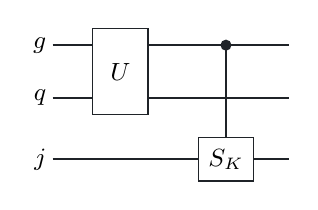
\begin{tikzpicture}[kme circuit]
\draw[kme wire] (0,1.45) node[left]{$g$} -- (3.0,1.45);
\draw[kme wire] (0,.78) node[left]{$q$} -- (3.0,.78);
\draw[kme wire] (0,0) node[left]{$j$} -- (3.0,0);
\node[kme gate,minimum height=11mm] at (.86,1.115) {$U$};
\draw[kme wire] (2.2,1.45) -- (2.2,0);
\node[kme dot] at (2.2,1.45) {};
\node[kme gate] at (2.2,0) {$S_K$};
\end{tikzpicture}\par\smallskip
{\small $S_K\ket j=\ket{j+1\bmod K}$.}
\end{minipage}\hfill
\begin{minipage}[t]{.48\linewidth}\centering
{\small\sffamily Measure only the guard tag}\par\medskip
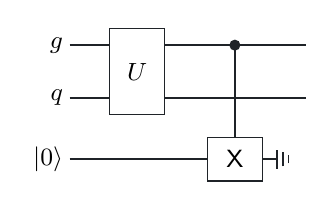
\begin{tikzpicture}[kme circuit]
\draw[kme wire] (0,1.45) node[left]{$g$} -- (3.0,1.45);
\draw[kme wire] (0,.78) node[left]{$q$} -- (3.0,.78);
\draw[kme wire] (0,0) node[left]{$\ket0$} -- (2.63,0);
\node[kme gate,minimum height=11mm] at (.86,1.115) {$U$};
\draw[kme wire] (2.10,1.45) -- (2.10,0);
\node[kme dot] at (2.10,1.45) {};
\node[kme gate] at (2.10,0) {$\mathsf X$};
\draw[kme wire] (2.64,-.12) -- (2.64,.12) (2.71,-.09) -- (2.71,.09)
(2.78,-.05) -- (2.78,.05);
\end{tikzpicture}\par\smallskip
{\small Discard the fresh bit after this call.}
\end{minipage}
\caption{One call to the same body $U$, followed by an operation
controlled on the outgoing guard $g=1$. A filled dot denotes a
coherent control. The left circuit carries $j$ into the next round.
In the right circuit the discarded bit distinguishes the tags without
distinguishing states of the payload $q$. Bare crossings have no
gate.}\label{fig:observe-circuit}
\Description{The guard controls either the cyclic successor on a
persistent counter or a bit flip on a fresh bit that is then
discarded.}
\end{programfigure}

\subsection{The same operations on sheets}
The finite counter in Figure~\ref{fig:76-finite-counter-sheet} uses
the depth of the page. The successor acts on its counter wire and
leaves the payload wire alone. Figures~\ref{fig:77-measured-sheet}
and~\ref{fig:75-phased-sheet} place the measurement and phase on that
return. Figure~\ref{fig:sheet-laws} shows how separate return sheets
compose, in the same upward orientation. In particular a seam labeled
$U$ acts on its incident summands even when one drawing of the
external wire is partially hidden by the returning surface.
\FloatBarrier

\section{A ring realization of the same exits}\label{sec:ring}
The reference circuit in Section~\ref{sec:trace} makes the scalar
phase observable. The same exits arise from an ideal lossless coupler
between an external waveguide mode and a circulating ring mode. Its
through amplitude is $t=3/5$ and its crossing amplitude $is$, where
$s=4/5$. Figure~\ref{fig:ring-model} gives its clauses and feedback
equation.

The coupler is $(1\oplus i)R_\theta(1\oplus(-i))$. Changing the
returning basis in this way gives entrance and exit coefficients both
equal to $is$, with return coefficient $t$. Their product on exit
$k+1$ is $(is)t^k(is)=-s^2t^k$, so every external exit is unchanged.
With phase $z$ per circuit, its single-frequency response is
therefore
$\Theta_{\rm ring}(z)=(t-z)/(1-tz)$, as for the rotation.
The same coupler has a literal rational-complex implementation:
\par\noindent\begin{minipage}{\linewidth}
\begin{lstlisting}
round ringCoupler : Unit + Unit = {
  exit unit <-> [3/5 . exit unit + (0 :+ 1) . 4/5 . back unit];
  back unit <-> [(0 :+ 1) . 4/5 . exit unit + 3/5 . back unit]
}

trace ringCoupler on unit
\end{lstlisting}
\end{minipage}\par
The command returns $-\ket*$, as does the guard rotation. The
returning basis change preserves every exit, not only their sum.

\begin{programfigure}
\begingroup
\definecolor{ringpass}{HTML}{007A59}
\definecolor{ringpasssoft}{HTML}{DAF1E9}
\definecolor{ringback}{HTML}{7A3E65}
\definecolor{ringbacksoft}{HTML}{F1E1EB}
\definecolor{ringlight}{HTML}{167BB4}
\begin{minipage}[t]{.30\linewidth}
{\footnotesize\itshape (a) the ring}\par\smallskip
\centering
\begin{tikzpicture}[x=9mm,y=9mm,>={Stealth[length=1.1mm,width=.8mm]},
every node/.style={font=\footnotesize,inner sep=1pt},line
width=.55pt]
 \filldraw[fill=ringbacksoft,draw=ringback] (0,1.18) circle (1.02);
 \filldraw[fill=white,draw=ringback] (0,1.18) circle (.78);
 \fill[ringpasssoft] (-1.8,-.12) rectangle (1.8,.12);
 \draw[ringpass] (-1.8,-.12)--(1.8,-.12) (-1.8,.12)--(1.8,.12);
 \draw[muted,dashed,rounded corners=1pt] (-.55,-.32) rectangle
 (.55,.45);
 \draw[ringlight,->,line width=.8pt] (-1.65,0)--(-.85,0);
 \draw[ringlight,->,line width=.8pt] (.85,0)--(1.65,0);
 \draw[ringlight,->,line width=.8pt] ($(0,1.18)+(-45:.9)$) arc
 (-45:215:.9);
 \node[text=ringback] at (0,1.18) {ring $Y$};
 \node[text=ringpass] at (1.55,.35) {$X$};
 \node[anchor=east] at (-1.82,0) {in};
 \node[anchor=west] at (1.82,0) {out};
 \node[text=muted] at (0,2.48) {one round takes $\tau_0$};
 \node[text=muted,anchor=north] at (0,-.50) {coupler};
\end{tikzpicture}
\end{minipage}\hfill
\begin{minipage}[t]{.31\linewidth}
{\footnotesize\itshape (b) one frequency}\par\smallskip
\centering
\begin{tikzpicture}[x=7mm,y=7mm,>={Stealth[length=1.1mm,width=.8mm]},
every node/.style={font=\footnotesize,inner sep=1pt},line
width=.55pt]
 \node[draw,shade,top color=white,bottom color=black!5,
minimum width=12mm,minimum height=13mm,font=\small] (cell) at (0,1.1)
{$C_{3/5}$};
 \draw[ringpass,->] (-2,1.45) node[left] {$u$} -- (cell.west |-
 0,1.45);
 \draw[ringpass,->] (cell.east |- 0,1.45) -- (2,1.45) node[right]
 {$v$};
 \node[draw=ringback,fill=ringbacksoft,inner xsep=3pt,inner ysep=3pt]
 (phase) at (0,-.9) {$z=e^{i\varphi}$};
 \draw[ringback,->] (cell.east |- 0,.75) -- (1.05,.75);
 \draw[ringback] (1.05,.75) to[out=0,in=0,looseness=1.25] (1.05,-.9)
 -- (phase.east);
 \draw[ringback] (phase.west) -- (-1.05,-.9)
 to[out=180,in=180,looseness=1.25] (-1.05,.75);
 \draw[ringback,->] (-1.05,.75) -- (cell.west |- 0,.75);
 \node[anchor=south] at (.95,.80) {$d$};
 \node[anchor=south] at (-.95,.80) {$y$};
 \node at (0,2.9) {$\binom v d=C_{3/5}\binom u y$};
 \node at (0,-1.85) {$y=zd$};
\end{tikzpicture}
\end{minipage}\hfill
\begin{minipage}[t]{.34\linewidth}
{\footnotesize\itshape (c) the source}\par\smallskip
\raggedright At $t=3/5$, $s=4/5$ the two outputs are
\[
\begin{aligned}
E* &\mapsto tE*+isB*,\\ B* &\mapsto isE*+tB* .
\end{aligned}
\]
$E$ is the waveguide and $B$ the ring.
\end{minipage}
\endgroup
\caption{The ring, the feedback equation at a single frequency, and
the two clauses of the coupler. Here $d$ is the amplitude leaving the
coupler inside the ring, and $y=zd$ enters it
again.}\label{fig:ring-model}
\Description{A ring beside one external waveguide, its stationary
feedback equation and corresponding iso.}
\end{programfigure}
In this lossless coupler~\cite[Eqs.~(6)--(7)]{Alsing17RingLoss}, the
observation depends on the input pulse. If the pulse lasts less than
one circuit time, the outgoing pulse on each round ends before the
next begins. Measuring the arrival time then distinguishes the exits
and gives their probabilities. At a single frequency all the
returning waves occupy the same mode and their amplitudes
add~\cite[Eqs.~(32)--(33)]{RaymerMcKinstrie13Cavity}.
Figure~\ref{fig:22-pulses} draws these two mode specifications.
\pic{22-pulses}{A short pulse leaves in distinct time bins, with exit
amplitudes $x_ku$. At one frequency the same exits contribute to one
outgoing mode and add coherently.}{Successive copies of a short input
pulse leave at different times, while a steady input receives their
coherent sum.}



Putting the bypass beside the ring gives the exits of
\code{withReference}. Prepare its external qubit in $\ket+$, run the
two arms, and apply $H$ to compare them. At resonance $z=1$, the
single-frequency response is $-1$ and the difference port has
probability $|1-(-1)|^2/4=1$. For a short pulse the first time bin
contributes $(1-t)^2/4$ to this port, and the later bins contribute
their probabilities separately:
\[
 \Pr(b=1)=\frac14\left((1-t)^2+
                \sum_{k\ge1}s^4t^{2(k-1)}\right)
=\frac14\bigl((1-t)^2+1-t^2\bigr)=\frac15.
\]
These are the coherent and measured predictions from
Section~\ref{sec:effects}. The scalar ring passes agreement, but the
two-arm body fails: its immediate exit contains the bypass and its
later exits do not. Forming that bypass uses a coherent sum of isos
before channelization, an operation unavailable to a channel context.

The two experiments specify different input and output modes, one
frequency or orthogonal time slots. A finite wave packet and
observation window require their own specification before these
predictions can be compared.


\section{Observing the response}\label{app:observing}

For a fixed $|z|=1$, the phase iso $P_z^c=\{s\leftrightarrow z\cdot
s\}_{s\in\mathcal B(c)}:c\leftrightarrow c$ gives the marked source
body $\beta;(I_b\oplus P_z^c)$. The bypass caller is
\[
H;\mathsf{trace}_1\bigl(\code{withReference}; (I_{\kw{Qubit}}\oplus
P_z^1)\bigr);H.
\]
Thus the phase variation used in the body of the paper is an ordinary
finite iso construction.

\paragraph{The controlled body.}
For $|z|=1$ and $\delta\in\mathbb R$, let the reference space be
$H_r=\C^2$, and put
$P_\delta=\operatorname{diag}(1,e^{i\delta})$.
Use distributivity to identify $H_r\otimes(X\oplus Y)$ with
$(H_r\otimes X)\oplus(H_r\otimes Y)$. The body in
Figure~\ref{fig:relative-hadamard} is the finite unitary
\[
W_{z,\delta} =\bigl(I_{H_r\otimes X'}\oplus(P_\delta\otimes
zI_Y)\bigr) (I_{H_r}\otimes U).
\]
It has external type $H_r\otimes X\to H_r\otimes X'$ and returning
summand $H_r\otimes Y$. For reference basis value $r=0$ its returning
phase is $z$, and for $r=1$ it is $ze^{i\delta}$. It never changes
that basis value. Its $k$th exit on the two sectors is therefore
respectively $z^kx_k$ and $(ze^{i\delta})^kx_k$. The closed gate is
\[
 \ket0\bra0_r\otimes\Theta(z)
+\ket1\bra1_r\otimes\Theta(ze^{i\delta}).
\]
For reference input $\ket+$ and unit data $u$, the closed gate
returns
\[
 \frac{\ket0_r\otimes\Theta(z)u+
           \ket1_r\otimes\Theta(ze^{i\delta})u}{\sqrt2}.
\]
Applying $S^\dagger$ and $H$ gives data vectors on reference outcomes
$0,1$:
$(\Theta(z)u-i\Theta(ze^{i\delta})u)/2$ and
$(\Theta(z)u+i\Theta(ze^{i\delta})u)/2$. Their squared-norm
difference is
$\operatorname{Im}\langle\Theta(z)u,\Theta(ze^{i\delta})u\rangle$.
Taylor expansion at $\delta=0$ gives the displayed derivative readout
in Figure~\ref{fig:relative-hadamard}.

Thus the straight reference line in the drawing denotes a tensor
factor carried on both alternative sheets. Its controlled phase acts
on each return. No coherent control of a channel hole is used.



At $z=1$, this construction compares $\Theta(1)u$ and
$\Theta(e^{i\delta})u$. For the scalar response $(3-5z)/(5-3z)$,
choose $\delta=\pi/2$. The imaginary overlap is $8/17$, so the two
outcome probabilities are $25/34$ and $9/34$. This finite-phase
readout is the exact overlap, whereas the derivative formula is its
first-order expansion at $\delta=0$. This specializes
Figure~\ref{fig:relative-hadamard} to the controlled body
$W_{1,\delta}$.
\end{document}

